\chapter{线性方程与矩阵方程}
\label{chap:linear-equations-and-optimization}
\label{sec:linear-algebra-reachability-solvability}

前面的章节建立了研究线性问题的工具：第~\ref{chap:linear-operations}章规定向量与矩阵的运算，
第~\ref{chap:linear-representation}章用列空间、零空间与秩描述线性映射，第~\ref{chap:normed-inner-product-spaces}章建立正交分解，
第~\ref{chap:linear-analysis}章用特征值、奇异值与条件数刻画矩阵作用的强弱方向和误差放大。
这些工具大多从正向计算出发：给定矩阵和输入，按乘法算出输出。实际问题常常反过来，
矩阵和希望得到的输出已经给定，要求找出输入。本章用前面的工具解决三个这样的具体问题。

第一个是线性方程$\bm A\bm x=\bm b$。面对一个具体的方程，先要判断它属于哪种情况：有唯一解、有无穷多解，还是没有解。
有没有解取决于$\bm b$是否落在列空间中，有几个解取决于零空间的大小，二者都可以用秩判别。
三种情况随后分别处理。有唯一解时，问题是怎样高效、稳定地把它算出来，不同结构的矩阵各有适合的分解。
有无穷多解时，要描述全部解，并说明若只报告一个，应当报告哪一个。
对于大规模方阵，还可以从初始近似出发，反复利用残差修正解；定常迭代固定修正规则，Krylov方法则随着当前信息选择修正。
没有解时，退而求其次，在所有能产生的输出中找离$\bm b$最近的一个，这就是最小二乘；这个问题又化为一个总有解的线性方程。

三种情况的答案最后由伪逆统一写出。以上讨论都假定数据精确。数据带有误差时，解会偏离多少，要用条件数回答。
小奇异值会使解对误差过于敏感，对此有两类改进：岭回归与截断SVD以改变问题为代价换取稳定；
修正Gram--Schmidt、Householder反射与Givens旋转不改变问题，只让计算本身少引入误差。

第二个是西尔维斯特（Sylvester）方程$\bm A\bm X+\bm X\bm B=\bm C$。它的未知量本身是一张矩阵，左右两侧的乘法同时作用在它上面。
把矩阵拉直成向量后，它又是一个线性方程，但系数矩阵的规模很大。因此我们不形成这个大矩阵，而是直接从$\bm A$、$\bm B$的特征值读出可解条件；
求解时，一般情况下利用它们的实Schur形，可对角化时则换到特征向量坐标直接写出解。

第三个是李雅普诺夫（Lyapunov）方程$\bm A\bm X+\bm X\bm A^\top=\bm Q$，它是Sylvester方程的对称特例。
解的对称性、对称性带来的计算节省以及解的正定性需要单独讨论；与之对应的离散型方程还有一个级数形式的解，正定性可以从中直接读出。

三个方程都按同样的顺序展开：方程表达什么问题，解是否存在、是否唯一，用什么方法求出；
线性方程还要回答求出的解怎样核验，以及数据带误差时解会偏离多少。

为便于比较，线性方程各节统一以$\bm A\in\mathbb R^{m\times d}$和$\bm b\in\mathbb R^m$为输入，以$\bm x\in\mathbb R^d$为未知量；方阵情形取$m=d$。精确解或选定的最小范数解记作$\bm x_\star$，迭代近似记作$\bm x_k$，残差统一取$\bm r_k=\bm b-\bm A\bm x_k$。最小二乘小节中的$\hat{\bm x}$表示使残差范数最小的解。分解因子、子空间坐标和辅助方向都是求解中的中间量，最终仍要回到原变量$\bm x$。

直接法的输入是矩阵与右端，输出是经原方程核验的解；迭代法还需初值、容差和最大步数，输出近似解、残差及停止原因。多个右端排成$\bm B=[\bm b_1\;\cdots\;\bm b_s]$时，问题写成$\bm A\bm X=\bm B$，各列分别遵循同样的步骤，并尽可能复用矩阵分解。后面的Sylvester方程另有左右两个系数矩阵，会在引入时重新说明它们的角色。

% 线性方程Ax=b（上）：问题、解的情况、唯一解的求解方法（分解、例子、比较与核验）、无穷多解（解集与最小范数解）

\section{线性方程的解结构}
\label{sec:ls-exact-linear-equations}
\label{sec:linear-algebra-exact-systems}

给定矩阵$\bm A\in\mathbb R^{m\times d}$与目标$\bm b\in\mathbb R^m$，线性方程要求找出输入$\bm x$，
使$\bm A$作用后的输出恰好等于目标：
\begin{equation}
\begin{gathered}
\bm A\bm x=\bm b\\
\bm x\in\mathbb R^d.
\end{gathered}
\label{eq:linear-algebra-linear-system}
\end{equation}
它由$m$个方程组成，含$d$个未知量。

若有$s$个目标$\bm b_1,\ldots,\bm b_s$共用同一个矩阵，
可以把它们排成$\bm B\in\mathbb R^{m\times s}$，把未知量排成$\bm X\in\mathbb R^{d\times s}$，
写成$\bm A\bm X=\bm B$。按矩阵乘法逐列读，这就是$s$个方程$\bm A\bm x_j=\bm b_j$并列。
每一列各自有解或无解，互不影响；它们只共享系数矩阵，因而可以共享对$\bm A$所做的计算。

本节先判断方程是否有解，再用零空间描述全部解；解不唯一时，以最小范数选出一个代表。求解算法从下一节开始讨论。

\subsection{方程是否有解}
\label{sec:ls-solution-cases}

按形状，$m=d$的方程称为方阵方程，$m>d$（方程多于未知量）称为超定，$m<d$（方程少于未知量）称为欠定。
一个自然的猜测是：超定方程无解，欠定方程多解，方阵方程恰有一解。下面的两个小方程说明这个猜测不成立。

\begin{example}[反例：形状不决定解的情况]
\label{ex:ls-shape-not-decisive}
超定方程
\[
 \begin{bmatrix}1\\1\end{bmatrix}x=\begin{bmatrix}1\\1\end{bmatrix}
\]
由两个相同的方程$x=1$组成，$x=1$是它的唯一解。方阵方程
\[
 \begin{bmatrix}1&1\\1&1\end{bmatrix}\bm x=\begin{bmatrix}1\\2\end{bmatrix}
\]
由$x_1+x_2=1$与$x_1+x_2=2$组成，两式左边相同而右边不同，互相矛盾，所以无解。
因此超定方程可以有唯一解，方阵方程也可以无解。
\end{example}

形状只限制了秩的上限：秩不超过$\min\{m,d\}$。有没有解要看$\bm b$与$\bm A$的列空间的关系，
有几个解要看$\bm A$的零空间，下面两段分别讨论。这里的“有解”指等式严格成立。
浮点计算中只能比较残差与容限，这一问题留到第~\ref{sec:ls-numerical-sensitivity}节；
算法报告失败，可能只是数值或实现上的问题，不能据此断定方程无解。

\paragraph{有解的条件}
\label{sec:ls-compatibility}

记$\bm a_1,\ldots,\bm a_d$为$\bm A$的各列。按矩阵乘法，$\bm A\bm x=x_1\bm a_1+\cdots+x_d\bm a_d$，
输入只提供组合系数。$\bm x$取遍$\mathbb R^d$时，输出恰好取遍列空间$\operatorname{range}(\bm A)$，所以
\[
 \bm A\bm x=\bm b\ \text{有解}\iff\bm b\in\operatorname{range}(\bm A).
\]
满足这一条件时称方程\term{相容}（consistent）。

为了能具体检验，把$\bm b$并到$\bm A$右侧，得到增广矩阵$[\bm A\;\bm b]$。
若$\bm b$已是原有列的组合，添上它不扩大列张成的空间，秩不变；否则新列带来一个新方向，秩恰好加一。因此
\begin{equation}
 \bm A\bm x=\bm b\ \text{相容}\iff
 \operatorname{rank}[\bm A\;\bm b]=\operatorname{rank}(\bm A).
 \label{eq:ls-augmented-rank}
\end{equation}
用示例~\ref{ex:ls-shape-not-decisive}中的方阵检验这一判据。

\begin{example}[增广矩阵的秩]
\label{ex:ls-augmented-rank-check}
取$\bm A=\left[\begin{smallmatrix}1&1\\1&1\end{smallmatrix}\right]$，它的两列相同，秩为$1$。右端取$\bm b=(1,2)^\top$时，
\[
 [\bm A\;\bm b]=\begin{bmatrix}1&1&1\\1&1&2\end{bmatrix}
\]
含线性无关的两列$(1,1)^\top$与$(1,2)^\top$，秩为$2>1$，所以方程无解，与示例~\ref{ex:ls-shape-not-decisive}的直接观察一致。
右端取$\bm b=(1,1)^\top$时，新列与原有的列相同，$[\bm A\;\bm b]$的秩仍为$1$，所以方程相容。
\end{example}

多右端方程$\bm A\bm X=\bm B$相容，当且仅当每一列$\bm b_j$都在列空间中，
即$\operatorname{rank}[\bm A\;\bm B]=\operatorname{rank}(\bm A)$。这些秩都可以用第~\ref{sec:ls-direct-methods}节的消元法求出。

\paragraph{解的个数}
\label{sec:ls-uniqueness-freedom}

方程相容以后，再问解有几个。若$\bm x_1,\bm x_2$都是解，则$\bm A(\bm x_1-\bm x_2)=\bm0$，两解之差落在零空间
$\operatorname{null}(\bm A)=\{\bm x:\bm A\bm x=\bm0\}$中；反过来，若$\bm x_0$是解且$\bm n\in\operatorname{null}(\bm A)$，
则$\bm A(\bm x_0+\bm n)=\bm b$，$\bm x_0+\bm n$也是解。所以方程相容时，任取一个解$\bm x_0$（称为特解），全部解恰为
\begin{equation}
 \bm x_0+\operatorname{null}(\bm A)=\{\bm x_0+\bm n:\bm n\in\operatorname{null}(\bm A)\}.
 \label{eq:ls-affine-solution-set}
\end{equation}
零空间只含零向量时解唯一；含有非零向量$\bm n$时，$\bm x_0+t\bm n$（$t\in\mathbb R$）已是无穷多个不同的解。
记$r=\operatorname{rank}(\bm A)$，由秩零度定理~\ref{thm:ls-rank-nullity}，$\dim\operatorname{null}(\bm A)=d-r$，
因此相容方程的解唯一，当且仅当$r=d$，即$\bm A$的$d$列线性无关，称为满列秩。

另一种满秩是$r=m$，称为满行秩。此时列空间是整个$\mathbb R^m$，任何右端都相容。
满行秩保证有解，满列秩保证有解时解唯一，下面的例子说明两种保证不能互换。

\begin{example}[反例：满行秩与满列秩互不蕴含]
\label{ex:ls-row-column-rank}
$1\times2$矩阵$\bm A=(1,1)$满行秩：方程$x_1+x_2=b$对每个$b$都有解；但$\bm A(1,-1)^\top=0$，
解可以沿$(1,-1)^\top$任意平移，不唯一。$2\times1$矩阵$\bm A=(1,1)^\top$满列秩：零空间只含零，有解必唯一；
但输出$x(1,1)^\top$的两个分量总相等，只有$\bm b\in\operatorname{span}\{(1,1)^\top\}$时才有解。
\end{example}

据此，超定方程即使满列秩，也只保证“有解则唯一”。欠定方程有$r\leq m<d$，有解时自由参数有$d-r\geq d-m\geq1$个，
所以从不唯一。方阵方程满秩时两种保证同时成立，对每个右端恰有一解，这正是$\bm A$可逆的情形。

\paragraph{方阵的行列式判据}
\phantomsection
\label{sec:ls-determinant-invertibility}
方阵是否可逆还可以由一个数判断。对$n$阶方阵$\bm A$，
\[
\begin{gathered}
\bm A\text{可逆}\iff\det\bm A\neq0\\
\bm A^{-1}=\frac{1}{\det\bm A}\operatorname{adj}(\bm A)\\
\det(\bm A^{-1})=\frac{1}{\det\bm A}.
\end{gathered}
\]

若$\bm A$可逆，由行列式的乘法性（第~\ref{sec:ls-determinant-properties}节），$\det\bm A\det(\bm A^{-1})=\det\bm I_n=1$，
所以$\det\bm A\neq0$，并得第三式。反过来，若$\det\bm A\neq0$，把古典伴随恒等式
$\bm A\operatorname{adj}(\bm A)=\operatorname{adj}(\bm A)\bm A=(\det\bm A)\bm I_n$（定理~\ref{thm:ls-adjugate-identity}）两边除以$\det\bm A$，
就得到一个从左、右两侧乘$\bm A$都给出$\bm I_n$的矩阵，即第二式。二阶时，第二式就是第~\ref{sec:prelim-inverse-matrices}节的二阶求逆公式。

\begin{example}[用伴随矩阵求二阶逆]
\label{ex:ls-adjugate-two-by-two}
取$\bm A=\left[\begin{smallmatrix}2&1\\0&3\end{smallmatrix}\right]$。$\det\bm A=2\cdot3-1\cdot0=6\neq0$，所以$\bm A$可逆。
二阶矩阵的古典伴随由交换两个对角元、两个非对角元变号得到，于是
\[
 \bm A^{-1}=\frac16\begin{bmatrix}3&-1\\0&2\end{bmatrix}.
\]
乘回可验$\bm A\bm A^{-1}=\frac16\left[\begin{smallmatrix}6&0\\0&6\end{smallmatrix}\right]=\bm I_2$，
并且$\det(\bm A^{-1})=\frac1{36}(3\cdot2-0)=\frac16=1/\det\bm A$。
\end{example}

$\det\bm A=0$的几何含义是：单位立方体被$\bm A$压扁成体积为零的形状，列空间不是整个$\mathbb R^n$，有的右端无解。
所以$n$阶方阵方程对每个右端恰有一解，当且仅当$\operatorname{rank}\bm A=n$，也当且仅当$\det\bm A\neq0$。
行列式适合作理论判据，实际判断与求解时并不展开行列式：排列展开有$n!$项，
而第~\ref{sec:ls-direct-methods}节的消元在求解的同时就读出了秩。

\paragraph{三种情况的秩判别}

把两方面合起来，记$\tilde r=\operatorname{rank}[\bm A\;\bm b]$。由于添上一列至多使秩加一，总有$\tilde r=r$或$\tilde r=r+1$，
方程恰属于下面三种情况之一：
\[
 \begin{aligned}
  \tilde r&=r+1: &&\text{无解};\\
  \tilde r&=r=d: &&\text{唯一解};\\
  \tilde r&=r<d: &&\text{无穷多解，全部解含}\ d-r\ \text{个自由参数}.
 \end{aligned}
\]
示例~\ref{ex:ls-augmented-rank-check}的方阵中$r=1<d=2$：
右端$(1,2)^\top$使$\tilde r=2$，属于无解；右端$(1,1)^\top$使$\tilde r=1$，属于无穷多解。
秩判别回答了解是否存在，下面进一步写出所有可能的解。

\subsection{全部解的表示}
\label{sec:ls-select-among-solutions}
\label{sec:linear-algebra-affine-relations}

第~\ref{sec:ls-uniqueness-freedom}节已经证明，全部解是$\bm x_0+\operatorname{null}(\bm A)$，
即把子空间$\operatorname{null}(\bm A)$平移到某个特解$\bm x_0$处得到的集合。这样的集合称为\term{仿射空间}（affine space）。
基点$\bm x_0$可以换成任何别的解，集合本身不变；方向空间$\operatorname{null}(\bm A)$则由集合唯一确定，
因为它恰好由集合中任意两点之差组成。例如$x_1+x_2=2$有特解$(1,1)^\top$，
零空间由$(1,-1)^\top$张成，全部解为$(1,1)^\top+t(1,-1)^\top$，$t\in\mathbb R$。

换个角度看，按“输出是否相同”把输入分组，同一组中任意两点之差都在零空间中，每组正是零空间的一个平移。
方程$\bm A\bm x=\bm b$的解集，就是输出为$\bm b$的那一组。
图~\ref{fig:vol1-add-linear-nullspace-fibers}以$\bm A=(1,1)$画出这种分组：
每条平行线$x_1+x_2=c$上的点产生同一个输出$c$。
\begin{figure}[!htb]
  \centering
  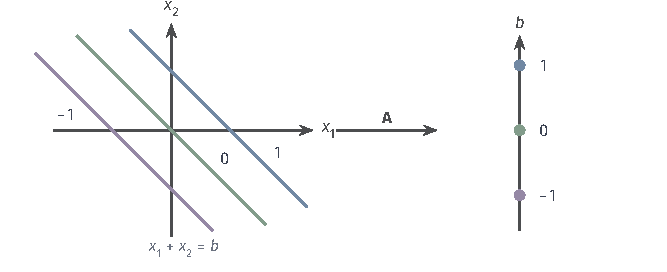
\includegraphics[width=112mm]{figures/00-shared/mathematical-preliminaries-upper/02-linear-spaces/tikz/comprehension-additions/linear-nullspace-fibers.pdf}
  \caption{同一输出对应的整组输入。对$\bm A=(1,1)$，蓝、绿、紫直线分别满足
  $x_1+x_2=1,0,-1$；右侧同色点是各直线的输出。绿色直线是$\ker\bm A$，
  其余直线是它的平移。把一整条直线归为一类后，才得到与可达输出的一一对应。}
  \label{fig:vol1-add-linear-nullspace-fibers}
\end{figure}

解集有多大，由零空间的维数决定。$\dim\operatorname{null}(\bm A)=d-r$，取零空间的一组基$\bm n_1,\ldots,\bm n_{d-r}$，
全部解可写成$\bm x_0+t_1\bm n_1+\cdots+t_{d-r}\bm n_{d-r}$，其中$t_1,\ldots,t_{d-r}$任意取值，
所以解集有$d-r$个自由参数。上例中$d=2$、$r=1$，自由参数只有$t$一个。

\paragraph{特解与零空间基的计算}

这一描述需要两样东西：一个特解和零空间的一组基。二者都可以从消元得到的阶梯形读出
（第~\ref{sec:ls-direct-methods}节）。主元所在的列对应主元变量，其余未知量称为自由变量，共$d-r$个。
把全部自由变量取零，回代解出主元变量，就得到一个特解；把右端换成零，令某一个自由变量取$1$、其余取零，
回代得到零空间中的一个向量，依次对每个自由变量这样做，得到的$d-r$个向量线性无关，构成零空间的一组基。
下面的例子按这一步骤计算。

\begin{example}[从阶梯形读出特解与零空间的基]
\label{ex:ls-particular-null-basis}
解
\[
 \begin{bmatrix}1&2&1\\2&4&3\end{bmatrix}\bm x=\begin{bmatrix}4\\9\end{bmatrix}.
\]
第二行减去第一行的$2$倍，得阶梯形
\[
 \begin{bmatrix}1&2&1\\0&0&1\end{bmatrix}\bm x=\begin{bmatrix}4\\1\end{bmatrix},
\]
即$x_3=1$。主元在第一、三列，$x_2$是自由变量，$r=2$、$d-r=1$。取$x_2=0$，
回代$x_1=4-2x_2-x_3=3$，得特解$\bm x_0=(3,0,1)^\top$。右端换成零并取$x_2=1$，得$x_3=0$、$x_1=-2$，
零空间由$\bm n=(-2,1,0)^\top$张成。所以全部解为
\[
\begin{gathered}
\bm x=(3-2t,\,t,\,1)^\top\\
t\in\mathbb R .
\end{gathered}
\]
代回可验$\bm A\bm x_0=(4,9)^\top$、$\bm A\bm n=\bm0$。
\end{example}

\subsection{相容方程的最小范数解}

方程本身给出的是整个仿射空间$\bm x_0+\operatorname{null}(\bm A)$，并不指定其中哪一个点。
若要报告一个确定的答案，必须另加准则。
最常用的准则是取欧氏范数最小的解，几何上就是在仿射空间中找离原点最近的点。

准则需要事先声明，因为不同准则选出的点不同：换一个内积，离原点“最近”的点一般也会改变。
示例~\ref{ex:ls-particular-null-basis}的特解$(3,0,1)^\top$也是一个合法的解，
只是它来自“自由变量取零”这一约定，换一种消元顺序就会得到另一个特解。

为求范数最小的点，把输入分成两部分：被$\bm A$消去的部分和真正决定输出的部分。
第一部分属于$\operatorname{null}(\bm A)$；第二部分应取在它的正交补中。
由定理~\ref{thm:ls-four-subspaces-orthogonality}，这个正交补就是行空间，$\operatorname{null}(\bm A)^\perp=\operatorname{range}(\bm A^\top)$，
输入空间有正交直和$\mathbb R^d=\operatorname{range}(\bm A^\top)\oplus\operatorname{null}(\bm A)$（式~\eqref{eq:ls-four-subspaces-decomposition}）：
$\operatorname{null}(\bm A)$是被消去的输入方向，$\operatorname{range}(\bm A^\top)$是真正影响输出的方向。

\paragraph{最小范数精确解的唯一性}

按输入空间的分解，每个解唯一写成$\bm x=\bm x_R+\bm x_N$，其中$\bm x_R\in\operatorname{range}(\bm A^\top)$，
$\bm x_N\in\operatorname{null}(\bm A)$。所有解共有同一个$\bm x_R$：若$\bm x'=\bm x'_R+\bm x'_N$是另一个解，
则$\bm x_R-\bm x'_R=(\bm x-\bm x')-(\bm x_N-\bm x'_N)$既在$\operatorname{range}(\bm A^\top)$中，
又是两个零空间向量之差，落在$\operatorname{null}(\bm A)$中；两个子空间互相正交，只交于零向量，故$\bm x_R=\bm x'_R$。
由于$\bm A\bm x_N=\bm0$，$\bm A\bm x_R=\bm A\bm x=\bm b$，$\bm x_R$本身也是解。两部分正交，勾股恒等式给出
\[
 \lVert\bm x\rVert_2^2=\lVert\bm x_R\rVert_2^2+\lVert\bm x_N\rVert_2^2\geq\lVert\bm x_R\rVert_2^2,
\]
等号当且仅当$\bm x_N=\bm0$。所以最小范数解存在且唯一，就是解集中落在$\operatorname{range}(\bm A^\top)$里的那一个。
用前面的直线方程核对这一刻画。

\begin{example}[直线$x_1+x_2=2$上的最小范数解]
\label{ex:ls-min-norm-line}
方程$x_1+x_2=2$的系数矩阵为$\bm A=(1,1)$，全部解为$(1+t,1-t)^\top$，$t\in\mathbb R$。它们的范数平方为
\[
 (1+t)^2+(1-t)^2=2+2t^2,
\]
在$t=0$时最小，所以最小范数解是$(1,1)^\top$。它正比于$\bm A^\top=(1,1)^\top$，确实落在$\operatorname{range}(\bm A^\top)$中。
\end{example}

\paragraph{最小范数解的计算}

这一刻画也给出计算方法。

设$\bm A$满行秩，要找的解形如$\bm x=\bm A^\top\bm w$，代入方程得
$\bm A\bm A^\top\bm w=\bm b$。$m$阶方阵$\bm A\bm A^\top$可逆：若$\bm A\bm A^\top\bm w=\bm0$，
则$\lVert\bm A^\top\bm w\rVert_2^2=\bm w^\top\bm A\bm A^\top\bm w=0$，即$\bm A^\top\bm w=\bm0$，
而$\bm A^\top$的$m$列线性无关，迫使$\bm w=\bm0$。于是最小范数解为
\[
 \bm x=\bm A^\top(\bm A\bm A^\top)^{-1}\bm b .
\]
实际计算时不形成逆矩阵：$\bm A\bm A^\top$对称正定，先用Cholesky分解解出$\bm w$，再算$\bm A^\top\bm w$。

\begin{example}[满行秩方程的最小范数解]
\label{ex:ls-min-norm-row-full-rank}
示例~\ref{ex:ls-particular-null-basis}的系数矩阵$\bm A=\left[\begin{smallmatrix}1&2&1\\2&4&3\end{smallmatrix}\right]$的秩为$2$，满行秩。计算
\[
 \bm A\bm A^\top=\begin{bmatrix}6&13\\13&29\end{bmatrix},
\]
解$\bm A\bm A^\top\bm w=(4,9)^\top$得$\bm w=(-1/5,2/5)^\top$，于是
\[
 \bm x=\bm A^\top\bm w=(3/5,\,6/5,\,1)^\top .
\]
它是全部解$(3-2t,t,1)^\top$中$t=6/5$的那一个，与零空间方向$(-2,1,0)^\top$正交。
它的范数平方为$14/5$，小于特解$(3,0,1)^\top$的范数平方$10$。
\end{example}

矩阵$\bm A^\top(\bm A\bm A^\top)^{-1}$从右边乘$\bm A$得到单位矩阵，是第~\ref{sec:prelim-inverse-matrices}节介绍过的右逆中的一个。
右逆不唯一，其他右逆给出的一般不是最小范数解。

\begin{example}[反例：其他右逆不给出最小范数解]
\label{ex:ls-other-right-inverse}
取$\bm A=(1,1)$。右逆$\bm A^\top(\bm A\bm A^\top)^{-1}=(1/2,1/2)^\top$把$b$送到最小范数解$(b/2,b/2)^\top$，范数为$|b|/\sqrt2$。
$(1,0)^\top$也满足$\bm A(1,0)^\top=1$，是另一个右逆；它把$b$送到$(b,0)^\top$。这也是方程的解，
但范数为$|b|$，$b\neq0$时大于最小范数。
\end{example}

形成$\bm A\bm A^\top$会把各行之间接近线性相关的程度放大（第~\ref{sec:ls-normal-equations-method}节对$\bm A^\top\bm A$说明了同样的现象）。
更可靠的做法是对$\bm A^\top$作第~\ref{chap:normed-inner-product-spaces}章的经济型QR分解~\eqref{eq:ls-qr-factorization}，
$\bm A^\top=\bm Q\bm R$，$\bm Q$是$d\times m$矩阵，$\bm R$是$m$阶可逆上三角矩阵。
最小范数解落在$\operatorname{range}(\bm A^\top)=\operatorname{range}(\bm Q)$中，可写成$\bm x=\bm Q\bm w$。
代入方程，$\bm A\bm x=\bm R^\top\bm Q^\top\bm Q\bm w=\bm R^\top\bm w=\bm b$，
这是下三角方程，前代即得$\bm w$。所得的解与上面的公式相同，但不形成$\bm A\bm A^\top$；
QR分解怎样稳定地计算，见第~\ref{sec:ls-orthogonalization-qr}节。

$\bm A$不满行秩时，有些方程可以由其他方程组合出来，$\bm A\bm A^\top$不可逆，上面的公式不能直接使用。
方程相容时，可以先删去这些多余的方程，化为满行秩的情形；要把最小范数解写成一个矩阵作用于$\bm b$，
则需要第~\ref{sec:ls-pseudoinverse}节的伪逆。

至此，无穷多解的情形已经回答：全部解是一个特解加零空间，二者都可由消元读出；
若只报告一个解，须声明准则，欧氏范数最小的解是解集中唯一落在$\operatorname{range}(\bm A^\top)$里的点，
满行秩时可由$\bm A\bm A^\top$的Cholesky分解或$\bm A^\top$的QR分解算出。
\section{直接求解}
\label{sec:ls-direct-methods}
\label{sec:linear-algebra-direct-exact}
\label{sec:matrix-analysis-stable-solvers}

本节讨论最常见的唯一解情形：$\bm A$是可逆方阵，对每个右端恰有一解。
超定而满列秩的方程在相容时也有唯一解，但判断它是否相容本身就要比较$\bm b$与列空间，
这与最小二乘的计算是同一件事，放到第~\ref{sec:ls-qr-method}节一并处理。

知道解唯一存在，还要把它算出来。三角方程最容易解：上三角方程的最后一个方程只含最后一个未知量，
解出后代入倒数第二个方程，又只剩一个未知量，如此从后向前逐个求出。

本节的方法都把一般方程化成三角方程，或化成规模更小的方程，在有限步内得到精确算术下的精确解，称为直接法。
它们需要整体读取矩阵并存储分解因子，适合矩阵规模可控、或同一矩阵要配多个右端的情形。

不同方法利用不同的矩阵结构。我们从一般方阵的消元出发，得到LU分解；对称正定矩阵可以省去一半运算，
得到Cholesky分解；对称但不定的矩阵用LDL$^{\top}$分解；具有分块结构或只作低秩修改的矩阵，
可以把大方程化成小方程。用正交变换化三角的QR分解同样能解方程，它与最小二乘一起在第~\ref{sec:ls-qr-method}节讨论。
最后把这些方法的适用条件和代价并列比较，并说明算出的解怎样核验。

\subsection{消元、主元与LU分解}

对一般可逆的$d$阶系数矩阵，目标是从$\bm A\bm x=\bm b$得到唯一的$\bm x$。直接写成$\bm A^{-1}\bm b$还没有说明怎样计算。消元的想法是同时变换系数和右端，把每个方程依赖的未知量逐渐减少，直到可以回代；LU分解则保存这些变换，以便换一个右端时继续使用。

高斯消元用一个方程的倍数去消另一个方程中的未知量。三种行变换——把某行的倍数加到另一行、交换两行、
某行乘非零常数——都可以逆转，因而不改变解集。先看一个二阶的例子。

\begin{example}[二阶方程的消元]
\label{ex:ls-elimination-two-by-two}
解
\[
 \begin{bmatrix}2&1\\4&3\end{bmatrix}\bm x=\begin{bmatrix}1\\3\end{bmatrix},
\]
即$2x_1+x_2=1$、$4x_1+3x_2=3$。第二个方程减去第一个方程的$2$倍，消去$x_1$，得$x_2=1$。
代回第一个方程，$2x_1+1=1$，得$x_1=0$。所以唯一解是$\bm x=(0,1)^\top$。
\end{example}

\paragraph{消元乘子与LU因子}

阶数较高时，消元按列进行，每一步把一列主对角线以下的元素全部消成零。下面的例子显示，
记下每一步所用的倍数，就得到矩阵的一个乘积分解。

\begin{example}[三阶消元与LU分解]
\label{ex:ls-lu-three-by-three}
考虑方程
\[
 \bm A\bm x=\begin{bmatrix}2&1&1\\4&3&3\\8&7&9\end{bmatrix}\bm x
 =\begin{bmatrix}3\\7\\19\end{bmatrix},
\]
先只对系数矩阵$\bm A$消元。第一步以$a_{1,1}=2$为主元，即用来做除数的元素。
第二行减去第一行的$l_{2,1}=4/2=2$倍，变为$(0,1,1)$；第三行减去第一行的$l_{3,1}=8/2=4$倍，变为$(0,3,5)$。
第二步以新的$(2,2)$元$1$为主元，第三行减去第二行的$l_{3,2}=3/1=3$倍，变为$(0,0,2)$。
消元结束时剩下上三角矩阵$\bm U$，三个乘子按位置填进单位下三角矩阵$\bm L$：
\[
\begin{gathered}
\bm L=\begin{bmatrix}1&0&0\\2&1&0\\4&3&1\end{bmatrix}\\
\bm U=\begin{bmatrix}2&1&1\\0&1&1\\0&0&2\end{bmatrix}.
\end{gathered}
\]
乘回可验$\bm L\bm U=\bm A$，例如$\bm L\bm U$的第三行是$4\cdot(2,1,1)+3\cdot(0,1,1)+(0,0,2)=(8,7,9)$。
\end{example}

图~\ref{fig:ls-lu-elimination-steps}画出这两步消元，以及乘子怎样按位置收集成$\bm L$。
乘回之所以能复原$\bm A$，是因为消元过程可以倒过来读。$\bm U$的第$i$行，是$\bm A$的第$i$行减去
若干个已经处理好的行（即$\bm U$的前$i-1$行）的倍数得到的，倍数就是乘子$l_{i,k}$：
\[
 \bm U_{i,:}=\bm A_{i,:}-\sum_{k<i}l_{i,k}\bm U_{k,:}
 \quad\Longrightarrow\quad
 \bm A_{i,:}=\sum_{k<i}l_{i,k}\bm U_{k,:}+1\cdot\bm U_{i,:}.
\]
右式说明$\bm A$的第$i$行是$\bm U$各行以$(l_{i,1},\ldots,l_{i,i-1},1,0,\ldots,0)$为系数的组合，
这正是$\bm L\bm U$的第$i$行。因此只要消元中不出现零主元，就有$\bm A=\bm L\bm U$，
其中$\bm L$是对角元为$1$的下三角矩阵，$\bm U$是上三角矩阵，称为LU分解。

有了分解，$\bm A\bm x=\bm b$就是$\bm L(\bm U\bm x)=\bm b$。

令$\bm z=\bm U\bm x$，先从前向后解下三角方程
$\bm L\bm z=\bm b$（前代），再从后向前解上三角方程$\bm U\bm x=\bm z$（回代）：
\begin{equation}
\begin{gathered}
z_i=b_i-\sum_{j<i}l_{i,j}z_j\\
x_i=\frac{z_i-\sum_{j>i}u_{i,j}x_j}{u_{i,i}}.
\end{gathered}
\end{equation}
下面用这两个公式完成示例~\ref{ex:ls-lu-three-by-three}的求解。

\begin{example}[用LU因子前代与回代]
\label{ex:ls-lu-forward-back}
沿用示例~\ref{ex:ls-lu-three-by-three}的因子$\bm L,\bm U$与右端$\bm b=(3,7,19)^\top$。前代解$\bm L\bm z=\bm b$：
\[
 \begin{gathered}
z_1=3\\
z_2=7-2\cdot3=1\\
z_3=19-4\cdot3-3\cdot1=4.
 \end{gathered}
\]
回代解$\bm U\bm x=\bm z$：
\[
 \begin{gathered}
x_3=\frac42=2\\
x_2=\frac{1-1\cdot x_3}{1}=-1,
 \end{gathered}
\]
\[
 x_1=\frac{3-1\cdot x_2-1\cdot x_3}{2}=1.
\]
代回原方程，$\bm A(1,-1,2)^\top=(3,7,19)^\top$，所以$\bm x=(1,-1,2)^\top$是方程的解。
\end{example}

前代算出的$\bm z$，正是消元过程对右端做同样变换的结果：例如$z_2=7-2\cdot3$，
就是第二行减去第一行的$2$倍时右端的变化。
\begin{figure}[!htb]
  \centering
  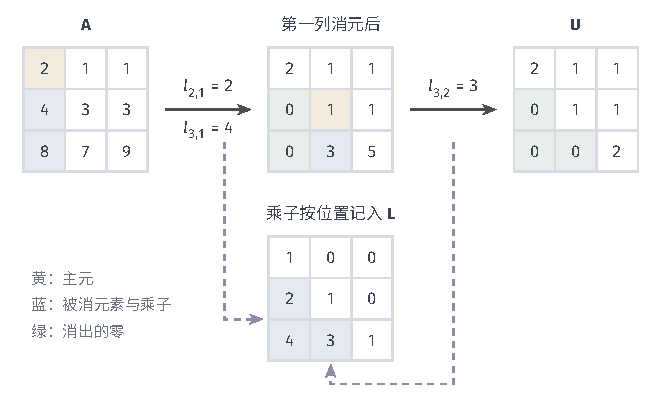
\includegraphics[width=112mm]{figures/00-shared/mathematical-preliminaries-upper/02-linear-spaces/tikz/comprehension-additions/linear-lu-elimination-steps.pdf}
  \caption{三阶矩阵的消元与LU因子。左起依次是$\bm A$、消去第一列后的矩阵与$\bm U$；
  黄色是当前主元，蓝色是待消去的元素，绿色是消出的零。箭头上的乘子等于被消元素除以主元，
  下方按原位置收集成单位下三角因子$\bm L$，满足$\bm L\bm U=\bm A$。}
  \label{fig:ls-lu-elimination-steps}
\end{figure}

\paragraph{选主元}

上面的做法要求每一步的主元不为零。可逆矩阵也可能在主元位置出现零，例如
$\left[\begin{smallmatrix}0&1\\1&1\end{smallmatrix}\right]$的$(1,1)$元为零，无法用它做除数；
交换两行后，以$1$为主元即可继续。主元不为零但很小时，问题同样存在，只是在浮点计算中才暴露出来。
下面的例子用只保留三位有效数字的算术显示这一点。

\begin{example}[小主元与行交换]
\label{ex:ls-partial-pivoting}
解$\left[\begin{smallmatrix}10^{-4}&1\\1&1\end{smallmatrix}\right]\bm x=(1,2)^\top$，
精确解为$x_1=1/(1-10^{-4})\approx1.0001$、$x_2=2-x_1\approx0.9999$。设每步运算结果
只保留三位有效数字（教学设定）。

不交换时，以$10^{-4}$为主元，乘子$l_{2,1}=10^4$。消元后右下角系数
$1-10^4=-9999$舍入为$-1.00\times10^4$，右端$2-10^4=-9998$也舍入为
$-1.00\times10^4$，得$x_2=1.00$，回代$x_1=(1-1.00)/10^{-4}=0$，第一分量完全错误：
大乘子把第二行原有的“$1$”和“$2$”淹没在$10^4$量级中。

先交换两行，以$1$为主元，乘子$l_{2,1}=10^{-4}$。消元后右下角系数$1-10^{-4}$与右端$1-2\times10^{-4}$
都舍入为$1.00$，得$x_2=1.00$，回代$x_1=2-1.00=1.00$，两分量在三位精度下都正确。
两种做法在精确算术中给出同一个解，区别只在乘子大小。
\end{example}

示例~\ref{ex:ls-partial-pivoting}说明，主元比同列其他元素小得多时，乘子会很大，舍入误差随之被放大。
因此第$k$步先在第$k$列尚未处理的元素中选绝对值最大的一个，把它所在的行换到主元位置，再消元。
这种做法称为部分主元，它保证每个乘子满足$|l_{i,k}|\leq1$。把全部行交换累计成置换矩阵$\bm P$，
得到带部分主元的LU分解
\begin{equation}
 \bm P\bm A=\bm L\bm U,
 \label{eq:matrix-analysis-palu}
\end{equation}
求解时先把右端按同样的方式重排，依次解$\bm L\bm z=\bm P\bm b$与$\bm U\bm x=\bm z$。

从输入到输出，带主元的算法可以按以下次序执行。
\begin{enumerate}
 \item 复制$\bm A$为工作矩阵，令$\bm P=\bm I$。对$k=1,\ldots,d-1$，在当前第$k$列的第$k$至$d$行选绝对值最大的主元，并交换相应两行。同步交换$\bm P$的两行，以及$\bm L$前$k-1$列中已记录的两行乘子。
 \item 对$i=k+1,\ldots,d$，用当前元素计算$l_{i,k}=a_{i,k}^{\mathrm{work}}/a_{k,k}^{\mathrm{work}}$，并对$j=k+1,\ldots,d$更新$a_{i,j}^{\mathrm{work}}\leftarrow a_{i,j}^{\mathrm{work}}-l_{i,k}a_{k,j}^{\mathrm{work}}$。处理完全部列后，上三角部分就是$\bm U$，乘子与单位对角线组成$\bm L$。
 \item 计算$\bm c=\bm P\bm b$，前代求$\bm z$，再回代求$\bm x$。最后计算$\bm b-\bm A\bm x$，其中使用的是原始系数与右端。
\end{enumerate}
这里主元选择和更新都使用工作矩阵的当前值，不再使用最初的$a_{i,j}$。在唯一解假设下，每一步都能找到非零主元；失去这一条件时，需要按下面的秩亏情形处理。

行交换只改变方程的排列次序，不改变解集。若示例~\ref{ex:ls-lu-three-by-three}也用部分主元，
第一步会把含$8$的第三行换到顶部，得到另一组$\bm P,\bm L,\bm U$，解不变。

行交换不会把奇异矩阵变成可逆矩阵。若某一步在精确算术下，当前列尚未处理的元素全为零，找不到非零主元，
说明这一列是前面主元列的组合，矩阵秩亏。这时跳过该列，继续处理下一列，最后得到阶梯形，非零主元的个数就是秩。

这样，消元同时回答了第~\ref{sec:ls-solution-cases}节的问题。
在阶梯形中，若某行左边全为零而右端非零，即出现$0=c\neq0$的矛盾行，方程不相容，这与增广矩阵的秩判据一致；
若没有矛盾行，把不对应主元的未知量（自由变量）取零，回代即得一个特解，其余解沿零空间展开，
具体做法见第~\ref{sec:ls-select-among-solutions}节。

浮点计算中，一个很小的主元并不能证明矩阵精确奇异：代数上的奇异（主元恰为零）与数值上的接近奇异
（主元很小但非零）是两回事，后者用数值秩描述，见第~\ref{sec:ls-numerical-sensitivity}节。

\paragraph{代价、复用与填充}

稠密$d\times d$矩阵的LU分解约需$2d^3/3$次浮点运算，$\bm L$与$\bm U$可以覆盖原矩阵存放，存储为$O(d^2)$。
分解完成后，每个右端只需前代与回代各一次，运算量为$O(d^2)$。所以同一个$\bm A$配多个右端$\bm b_j$时，
分解只做一次，此后每列只付$O(d^2)$的代价。复用的前提是矩阵不变；矩阵元素一旦改变，旧的$\bm L\bm U$
不再等于新的$\bm P\bm A$，必须重新分解，或改用后文的低秩更新。

稀疏矩阵的情形更微妙。消元会在原来为零的位置产生非零元，称为\term{填充}（fill-in），
使原本稀疏的因子变得接近稠密。填充的多少取决于消元顺序，下面的箭头形矩阵说明这一点。

\begin{example}[箭头形矩阵的填充]
\label{ex:ls-arrow-fill-in}
考虑一个$5\times5$矩阵，其中一个变量与其余全部变量耦合，其余变量彼此不耦合，
非零元只在对角线和这个变量对应的行与列上。

若先消去这个变量，要从其余每一行减去它所在行的倍数，而这一行在所有列上都有非零元，
所以剩下的$4\times4$块全部变成非零：原来只有$4$个对角非零元，现在有$16$个，新增的$12$个都是填充。
若把它排到最后，消去前四个变量时，每一步只改动右下角那一个元素，不产生任何填充。

推广到$n$阶，前一种顺序使因子变为稠密，需存约$n^2$个元素，分解约需$O(n^3)$次运算；
后一种只需原有的$3n-2$个元素和$O(n)$次运算。
\end{example}

图~\ref{fig:ls-sparse-fill-in-ordering}并置了两种顺序。矩阵和解都相同，代价却随顺序相差悬殊，
所以稀疏直接法先选消元顺序、再作分解，其代价也不能只按原始非零元数估计。
\begin{figure}[!htb]
  \centering
  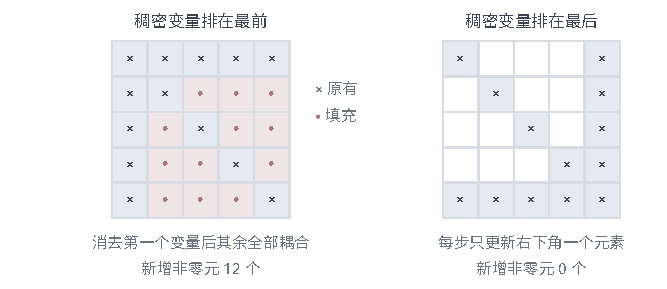
\includegraphics[width=112mm]{figures/00-shared/mathematical-preliminaries-upper/02-linear-spaces/tikz/comprehension-additions/linear-sparse-fill-in-ordering.pdf}
  \caption{消元顺序决定填充。同一个“箭头形”矩阵：左图把与全部变量耦合的变量排在最前，
  消去它后其余位置全部变为非零（红点为填充）；右图把它排在最后，因子保持原有稀疏结构。
  蓝格是原矩阵的非零元。}
  \label{fig:ls-sparse-fill-in-ordering}
\end{figure}

\subsection{正定方程与Cholesky分解}

很多方程的系数矩阵是对称正定的，例如第~\ref{sec:ls-least-squares}节满列秩时的$\bm A^\top\bm A$。
对这类矩阵，LU分解有两处浪费：$\bm U$与$\bm L$实际上携带同样的信息（$\bm U$的第$i$行是$\bm L^\top$的第$i$行乘以第$i$个主元），却要分别计算和存储；
部分主元的行交换会破坏对称性，而对称正定矩阵其实不需要交换。下面说明，对称正定矩阵可以写成
$\bm L\bm L^\top$，只算一个三角因子，并且不必选主元。

设$\bm A=\bm A^\top\succ0$。把第一行、第一列与其余部分分开，也把待求的下三角因子同样分块：
\[
\begin{gathered}
\bm A=\begin{bmatrix}a_{1,1}&\bm a^\top\\\bm a&\bm A_{22}\end{bmatrix}\\
\bm L=\begin{bmatrix}l_{1,1}&\bm0\\\bm l&\bm L_{22}\end{bmatrix}\\
\bm L\bm L^\top=\begin{bmatrix}l_{1,1}^2&l_{1,1}\bm l^\top\\ l_{1,1}\bm l&\bm l\bm l^\top+\bm L_{22}\bm L_{22}^\top\end{bmatrix}.
\end{gathered}
\]
令$\bm L\bm L^\top=\bm A$并逐块比较：左上角要求$l_{1,1}^2=a_{1,1}$。正定性给出
$a_{1,1}=\bm e_1^\top\bm A\bm e_1>0$，故可取$l_{1,1}=\sqrt{a_{1,1}}>0$。左下角要求$\bm l=\bm a/l_{1,1}$。
右下角要求
\[
 \bm L_{22}\bm L_{22}^\top=\bm A_{22}-\bm l\bm l^\top=\bm A_{22}-\frac{\bm a\bm a^\top}{a_{1,1}},
\]
问题化为对低一阶的矩阵$\bm A_{22}-\bm a\bm a^\top/a_{1,1}$做同样的分解。

这个剩余矩阵仍然对称正定。对任意非零$\bm u$，取$\bm x=(-\bm a^\top\bm u/a_{1,1},\,\bm u)$，它非零，展开可得
$\bm x^\top\bm A\bm x=\bm u^\top(\bm A_{22}-\bm a\bm a^\top/a_{1,1})\bm u$，而左边为正。
右边正是对第一个变量配方后剩下的二次型。于是同样的论证可以一阶一阶做下去，每一步开方的数都严格为正。
定理~\ref{thm:ls-gram-factor}用同样的配方归纳证明了正定矩阵可写成$\bm L^\top\bm L$的形式，
那里的上三角因子就是这里的$\bm L^\top$；这里把同一构造落实为逐列计算的算法。

\paragraph{Cholesky因子的逐列构造}

总结起来，对称正定矩阵$\bm A$存在唯一的对角元为正的下三角矩阵$\bm L$，使
\begin{equation}
 \bm A=\bm L\bm L^\top,
 \label{eq:matrix-analysis-cholesky}
\end{equation}
称为\term{Cholesky分解}（Cholesky decomposition）。上面的分块递推展开成逐元素的形式，就是按列计算
\begin{equation}
\begin{gathered}
l_{j,j}=\sqrt{a_{j,j}-\sum_{k<j}l_{j,k}^2}\\
l_{i,j}=\frac{a_{i,j}-\sum_{k<j}l_{i,k}l_{j,k}}{l_{j,j}}\quad(i>j).
\end{gathered}
\end{equation}
两式都来自比较$\bm L\bm L^\top$与$\bm A$的元素：$\bm L\bm L^\top$的$(i,j)$元（$i\geq j$）是
$\sum_{k\leq j}l_{i,k}l_{j,k}$，其中$k<j$的项只含前面各列，已经算出；剩下的一项$l_{i,j}l_{j,j}$
（$i=j$时是$l_{j,j}^2$）便可解出。根号内的数是第$j$步配方后的剩余，正定性保证它严格为正。
唯一性也由此可见：每个元素都被唯一解出，只有开方有正负两种选择，约定对角元为正就排除了这一任意性。
下面按这两个公式算一个三阶的例子。

\begin{example}[逐列计算Cholesky因子]
\label{ex:ls-cholesky-three-by-three}
取对称矩阵
$\bm A=\left[\begin{smallmatrix}4&2&2\\2&5&3\\2&3&6\end{smallmatrix}\right]$。
第一列：$l_{1,1}=\sqrt4=2$，$l_{2,1}=2/2=1$，$l_{3,1}=2/2=1$。此时剩余矩阵为
\[
 \begin{bmatrix}5&3\\3&6\end{bmatrix}-\begin{bmatrix}1&1\\1&1\end{bmatrix}
 =\begin{bmatrix}4&2\\2&5\end{bmatrix}.
\]
第二列：$l_{2,2}=\sqrt{5-l_{2,1}^2}=\sqrt4=2$，$l_{3,2}=(3-l_{3,1}l_{2,1})/l_{2,2}=(3-1)/2=1$。
第三列：$l_{3,3}=\sqrt{6-l_{3,1}^2-l_{3,2}^2}=\sqrt4=2$。于是
\[
 \bm L=\begin{bmatrix}2&0&0\\1&2&0\\1&1&2\end{bmatrix},
\]
乘回$\bm L\bm L^\top$逐项等于$\bm A$。三个根号内的数都是$4$，都为正。
\end{example}

在精确算术下，计算本身也是正定性的检验。若每一步根号内的数都为正，就得到可逆的$\bm L$，
于是对非零$\bm x$有$\bm x^\top\bm A\bm x=\lVert\bm L^\top\bm x\rVert_2^2>0$，$\bm A$正定；
反之，若某一步根号内出现零或负数，$\bm A$就不是正定的。示例~\ref{ex:ls-cholesky-three-by-three}的计算因此同时证明了$\bm A$正定。浮点运算中，接近零的配方剩余可能受到舍入影响，因此分解是否成功只能作为数值判断，还须结合误差尺度。

求解时，依次解$\bm L\bm z=\bm b$（前代，$z_i=(b_i-\sum_{j<i}l_{i,j}z_j)/l_{i,i}$）与
$\bm L^\top\bm x=\bm z$（回代，$x_i=(z_i-\sum_{j>i}l_{j,i}x_j)/l_{i,i}$）。

\begin{example}[用Cholesky因子求解]
\label{ex:ls-cholesky-solve}
沿用示例~\ref{ex:ls-cholesky-three-by-three}的$\bm A$与$\bm L$，取右端$\bm b=(8,10,11)^\top$。前代解$\bm L\bm z=\bm b$：
\[
 \begin{gathered}
z_1=\frac82=4\\
z_2=\frac{10-1\cdot4}{2}=3\\
z_3=\frac{11-1\cdot4-1\cdot3}{2}=2.
 \end{gathered}
\]
回代解$\bm L^\top\bm x=\bm z$：
\[
 \begin{gathered}
x_3=\frac22=1\\
x_2=\frac{3-1\cdot1}{2}=1\\
x_1=\frac{4-1\cdot1-1\cdot1}{2}=1.
 \end{gathered}
\]
代回可验$\bm A(1,1,1)^\top=(8,10,11)^\top$，所以$\bm x=(1,1,1)^\top$。
\end{example}

稠密情形的运算量约为$d^3/3$，是LU的一半；存储也只需一个三角因子，约$d^2/2$个元素。多个右端同样复用一次分解。

矩阵只是半正定时，某一步的配方剩余可能恰为零，后续除以$l_{j,j}$就无法进行。
这时不应随手给对角线加一个小常数让计算通过，那样解的已经是另一个方程。
应先分清原因：$\bm A$本身有零空间时，方程不再有唯一解，回到第~\ref{sec:ls-solution-cases}节判断它属于哪种情况；
剩余量只是因舍入而接近零时，属于数值问题，见第~\ref{sec:ls-numerical-sensitivity}节。
只有任务本身要求加入惩罚项时，才改解相应的正则化方程（第~\ref{sec:ls-regularized-ls}节）。

\subsection{对称不定方程与分块LDL分解}
\label{sec:ls-ldlt}

对称但不定的矩阵，既有使二次型为正的方向，也有使它为负的方向。前面已经说明，逐列计算成功就证明矩阵正定，
所以对不定矩阵，Cholesky的开方必定在某一步遇到非正的数。下面是最小的例子。

\begin{example}[反例：不定矩阵的Cholesky中断]
\label{ex:ls-cholesky-indefinite}
取$\bm A=\left[\begin{smallmatrix}1&2\\2&1\end{smallmatrix}\right]$。它对称，$\det\bm A=-3\neq0$，所以可逆；
但$\bm x=(1,-1)^\top$给出$\bm x^\top\bm A\bm x=1-4+1=-2<0$，$\bm A$不定。按Cholesky的逐列公式，
第一列得$l_{1,1}=1$、$l_{2,1}=2$，第二列要求
\[
 l_{2,2}=\sqrt{a_{2,2}-l_{2,1}^2}=\sqrt{1-2^2}=\sqrt{-3},
\]
在实数中无法进行。
\end{example}

我们仍想利用对称性，只算一个三角因子。办法是不开方，把每一步的主元单独放进对角矩阵$\bm D$，负号就留在$\bm D$里。

\paragraph{LDL$^{\top}$因子的形成}

仍以示例~\ref{ex:ls-cholesky-indefinite}的矩阵为例，看不开方时消元记录下什么。

\begin{example}[二阶不定矩阵的LDL$^{\top}$分解]
\label{ex:ls-ldlt-two-by-two}
对$\bm A=\left[\begin{smallmatrix}1&2\\2&1\end{smallmatrix}\right]$，以$a_{1,1}=1$为主元，乘子$l_{2,1}=2/1=2$，
消元后剩余系数为$1-2\cdot2=-3$。把乘子放进单位下三角矩阵，把两个主元$1$与$-3$放进对角矩阵，得
\[
 \bm A=\begin{bmatrix}1&0\\2&1\end{bmatrix}
 \begin{bmatrix}1&0\\0&-3\end{bmatrix}
 \begin{bmatrix}1&2\\0&1\end{bmatrix}=\bm L\bm D\bm L^\top .
\]
乘回可验等式成立。剩余系数$-3$原样保留在$\bm D$中，不需要开方。
\end{example}

这就是LDL$^{\top}$分解的基本形式：$\bm L$是单位下三角矩阵，$\bm D$是对角矩阵。

只用一阶主元并不总够，下面的矩阵就没有可用的一阶主元。

\begin{example}[反例：没有一阶主元的对称可逆矩阵]
\label{ex:ls-no-scalar-pivot}
取$\bm A=\left[\begin{smallmatrix}0&1\\1&0\end{smallmatrix}\right]$。$\det\bm A=-1\neq0$，所以$\bm A$可逆；
但两个对角元都是零，没有一个能作除数。若像LU那样交换两行，得到的是$\bm P\bm A=\bm L\bm U$形式的分解，
不再是对称的$\bm L\bm D\bm L^\top$。若对称地交换，即同时交换两行和对应的两列，结果仍是$\bm A$本身：
对称置换只重新排列对角元，而这里的对角元全为零。
\end{example}

所以解决办法有两条。一是对称地交换，矩阵仍然对称，对角元被重新排列；若其他位置有合适的对角元，
就可以把它换到主元位置。二是允许用$2\times2$的对称可逆块作主元，在对角元都不合适时必须这样做：
示例~\ref{ex:ls-no-scalar-pivot}的整个矩阵就是一个可逆的二阶块，直接把它放进$\bm D$即可。
一般地，把对称置换累计成$\bm P$，得到
\[
 \bm P\bm A\bm P^\top=\bm L\bm D\bm L^\top,
\]
其中$\bm L$单位下三角，$\bm D$由一阶与二阶对角块组成。

计算过程与LU相同，只是按块进行。把当前待处理的矩阵分块为
$\left[\begin{smallmatrix}\bm A_{11}&\bm A_{21}^\top\\\bm A_{21}&\bm A_{22}\end{smallmatrix}\right]$，
其中$\bm A_{11}$是选定的可逆一阶或二阶主元块。正如标量消元用乘子$l_{i,k}=a_{i,k}/a_{k,k}$，
块消元的乘子块是$\bm L_{21}=\bm A_{21}\bm A_{11}^{-1}$；从下面的块行中减去$\bm L_{21}$乘主元块行，
左下块变成零，右下块变成
\[
 \bm A_{22}-\bm L_{21}\bm A_{21}^\top=\bm A_{22}-\bm A_{21}\bm A_{11}^{-1}\bm A_{21}^\top ,
\]
它仍是对称矩阵，对它重复同样的过程。$\bm L$收集各步的乘子块，$\bm D$收集各步的主元块。
每一步都可以把$\bm L\bm D\bm L^\top$乘回，核对它是否等于置换后的矩阵。

求解时先把右端按$\bm P$重排，再依次解下三角方程$\bm L\bm z=\bm P\bm b$、
块对角方程$\bm D\bm y=\bm z$与上三角方程$\bm L^\top\bm w=\bm y$，最后令$\bm x=\bm P^\top\bm w$还原次序。
其中块对角方程逐块求解：一阶块$d$直接得$y=z/d$；二阶块
$\left[\begin{smallmatrix}d_{11}&d_{12}\\d_{12}&d_{22}\end{smallmatrix}\right]$
的行列式$\Delta=d_{11}d_{22}-d_{12}^2$因主元块可逆而非零，由二阶逆矩阵公式得
\begin{equation}
\begin{gathered}
y_1=\frac{d_{22}z_1-d_{12}z_2}{\Delta}\\
y_2=\frac{d_{11}z_2-d_{12}z_1}{\Delta}.
\end{gathered}
\end{equation}
示例~\ref{ex:ls-no-scalar-pivot}的二阶块有$\Delta=-1$，代入得$y_1=z_2$、$y_2=z_1$，
两个未知量一次解出。与Cholesky相比，这一求解过程只是在两次三角求解之间插入了块对角求解，并多了置换与还原；
运算量同样约为$d^3/3$。

例如给示例~\ref{ex:ls-ldlt-two-by-two}配上右端$\bm b=(3,3)^\top$，此时无需置换。前代$\bm L\bm z=\bm b$得$\bm z=(3,-3)^\top$；块对角求解$\bm D\bm y=\bm z$得$\bm y=(3,1)^\top$；最后回代$\bm L^\top\bm x=\bm y$得$\bm x=(1,1)^\top$。代入原来的不定矩阵，得到$\bm A\bm x=(3,3)^\top$。负主元只改变中间方程的系数，并不妨碍求解。

最后要分清$\bm D$中的两种情况。负的对角元或不定的二阶块表示矩阵有负方向，但它们可逆，
方程照样唯一可解；零块则表示矩阵奇异，不能当作可逆块做除法，需要回到第~\ref{sec:ls-solution-cases}节重新判断解的情况。

\subsection{分块消元与Schur补}
\label{sec:matrix-analysis-blocks-updates}

LDL$^{\top}$分解中的块消元有更广的用途。若未知量可以自然地分成两组，而且消去其中一组很便宜，
就可以先消去它，只解剩下那组未知量满足的较小方程。先看每组只有一个未知量的最小例子。

\begin{example}[二阶方程的分块消元]
\label{ex:ls-block-elimination-two-by-two}
解$\left[\begin{smallmatrix}2&1\\1&2\end{smallmatrix}\right](x_1,x_2)^\top=(1,3)^\top$。
第一个方程$2x_1+x_2=1$给出$x_1=(1-x_2)/2$。代入第二个方程$x_1+2x_2=3$，得
\[
\begin{gathered}
\frac{1-x_2}{2}+2x_2=3\\
\text{即}\qquad \frac32x_2=3-\frac12=\frac52,
\end{gathered}
\]
故$x_2=5/3$，回代得$x_1=(1-5/3)/2=-1/3$。核验：$2(-1/3)+5/3=1$，$(-1/3)+2(5/3)=3$。
消去$x_1$后，$x_2$的系数从$2$变成$2-1\cdot\tfrac12\cdot1=\tfrac32$，右端从$3$变成$3-1\cdot\tfrac12\cdot1=\tfrac52$。
\end{example}

图~\ref{fig:ls-schur-block-elimination}把这两步并置。下面把标量换成块，看系数与右端的这两处变化在一般情形下是什么。

\begin{figure*}[htbp]
  \centering
  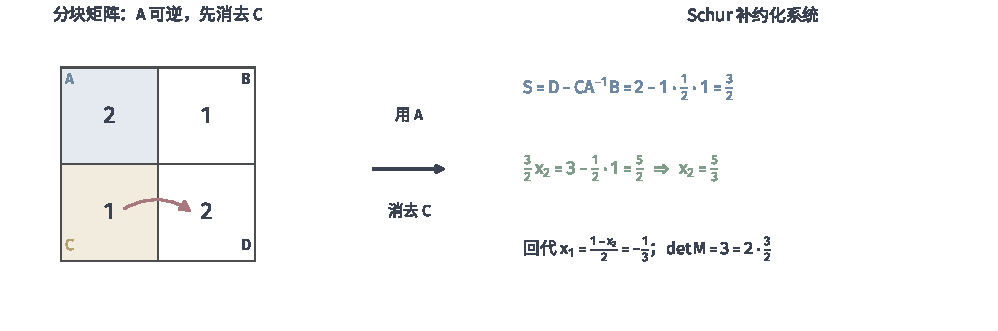
\includegraphics[width=168.998mm]{figures/00-shared/mathematical-preliminaries-upper/02-linear-spaces/matplotlib/ls-schur-block-elimination/ls-schur-block-elimination.pdf}
  \caption{Schur 补的 2×2 分块消元。左：$\bm M=\left[\begin{smallmatrix}2&1\\1&2\end{smallmatrix}\right]$
  按左上块$\bm A=2$分块，先由第一行表出$x_1=(1-x_2)/2$；右：代入第二行后右下角残留
  Schur补$\bm S=3/2$，约化得$x_2=5/3$、回代$x_1=-1/3$，且$\det\bm M=2\cdot3/2=3$。
  解析式教学构造。}
  \label{fig:ls-schur-block-elimination}
\end{figure*}

\paragraph{Schur补与约化系统}

这里仍然求解同一个$\bm A\bm x=\bm b$问题，只是把系数、未知量和右端各分成两组。为沿用常见的块公式，下面临时把整体系数记为$\bm M$，把它的四个块记为$\bm A,\bm B,\bm C,\bm D$；整体未知量和右端分别是$(\bm x^\top,\bm y^\top)^\top$与$(\bm f^\top,\bm g^\top)^\top$。这些块由原输入分割得到，并不是新的待估参数。

设分块方程为
\[
 \begin{bmatrix}\bm A&\bm B\\\bm C&\bm D\end{bmatrix}
 \begin{bmatrix}\bm x\\\bm y\end{bmatrix}
 =\begin{bmatrix}\bm f\\\bm g\end{bmatrix},
\]
系数矩阵记为$\bm M$，其中$\bm A\in\mathbb R^{p\times p}$可逆。第一组方程$\bm A\bm x+\bm B\bm y=\bm f$
给出$\bm x=\bm A^{-1}(\bm f-\bm B\bm y)$；代入第二组$\bm C\bm x+\bm D\bm y=\bm g$，得
$\bm C\bm A^{-1}\bm f-\bm C\bm A^{-1}\bm B\bm y+\bm D\bm y=\bm g$。整理后，$\bm y$满足
\begin{equation}
\begin{gathered}
\bm S\bm y=\bm g-\bm C\bm A^{-1}\bm f\\
\bm S=\bm D-\bm C\bm A^{-1}\bm B.
\end{gathered}
\label{eq:matrix-analysis-schur-complement}
\end{equation}
矩阵$\bm S$称为$\bm A$在$\bm M$中的\term{Schur补}（Schur complement），方程~\eqref{eq:matrix-analysis-schur-complement}
称为约化系统。

若要据此编写求解过程，输入四个块与两个右端后，先分解被消去的块$\bm A$，复用其因子解
\[
 \bm A\bm Z=\bm B,\qquad \bm A\bm u=\bm f.
\]
再形成$\bm S=\bm D-\bm C\bm Z$及$\bm h=\bm g-\bm C\bm u$，解小方程$\bm S\bm y=\bm h$，最后恢复$\bm x=\bm u-\bm Z\bm y$。输出是两组未知量合并后的向量；若只停在Schur补$\bm S$，还没有完成原问题的求解。
\label{def:matrix-analysis-schur-complement}
示例~\ref{ex:ls-block-elimination-two-by-two}相当于取$\bm A=2$、$\bm B=\bm C=1$、$\bm D=2$、$\bm f=1$、$\bm g=3$，
此时$\bm S=2-1/2=3/2$，约化系统的右端为$3-1/2=5/2$，与那里算出的系数和右端一致。
Cholesky每一步的剩余矩阵$\bm A_{22}-\bm a\bm a^\top/a_{1,1}$，以及LDL$^{\top}$每一步的右下块，都是这样的Schur补。

同一过程写成矩阵乘法，是左乘一个单位块下三角矩阵，消去左下块：
\[
 \begin{bmatrix}\bm I&\bm0\\-\bm C\bm A^{-1}&\bm I\end{bmatrix}
 \begin{bmatrix}\bm A&\bm B\\\bm C&\bm D\end{bmatrix}
 =\begin{bmatrix}\bm A&\bm B\\\bm0&\bm S\end{bmatrix}.
\]
左边第一个因子的行列式为$1$，右边是块上三角矩阵，所以$\det\bm M=\det\bm A\det\bm S$。
因此在$\bm A$可逆的前提下，$\bm M$可逆当且仅当$\bm S$可逆。示例~\ref{ex:ls-block-elimination-two-by-two}中$\det\bm M=3=2\cdot\tfrac32$。

计算时，先解约化系统得到$\bm y$，再回代$\bm x=\bm A^{-1}(\bm f-\bm B\bm y)$。其中凡是出现$\bm A^{-1}$的地方，
都通过对$\bm A$的分解求解来实现，例如$\bm A^{-1}\bm B$由解$\bm A\bm Z=\bm B$得到，不必先形成逆矩阵。
这种做法的典型来源是二部结构：少量全局未知量与大量局部未知量相连，局部未知量彼此之间不直接耦合。
这时$\bm A$是块对角的，消去局部块很便宜，只剩下全局未知量的小系统。

若需要整个逆矩阵，把上述消元过程对一般右端做完，可得块逆公式
\begin{equation}
 \bm M^{-1}=
 \begin{bmatrix}
  \bm A^{-1}+\bm A^{-1}\bm B\bm S^{-1}\bm C\bm A^{-1}
  &-\bm A^{-1}\bm B\bm S^{-1}\\
  -\bm S^{-1}\bm C\bm A^{-1}&\bm S^{-1}
 \end{bmatrix}.
 \label{eq:matrix-analysis-block-inverse}
\end{equation}

$\bm M$对称时$\bm C=\bm B^\top$，Schur补还能判断正定性。对二次型配方：
\begin{equation}
 \begin{aligned}
 &\begin{bmatrix}\bm x\\\bm y\end{bmatrix}^{\top}
 \bm M\begin{bmatrix}\bm x\\\bm y\end{bmatrix}\\
 &=\bm x^\top\bm A\bm x+2\bm x^\top\bm B\bm y+\bm y^\top\bm D\bm y\\
 &=(\bm x+\bm A^{-1}\bm B\bm y)^\top
 \bm A(\bm x+\bm A^{-1}\bm B\bm y)+\bm y^\top\bm S\bm y.
 \end{aligned}
\end{equation}
展开右边第一项即可验证第二个等号，它多出的$\bm y^\top\bm B^\top\bm A^{-1}\bm B\bm y$正好被$\bm S=\bm D-\bm B^\top\bm A^{-1}\bm B$
中的减项抵消。于是在$\bm A\succ0$时
\begin{equation}
 \bm M\succ0\quad\Longleftrightarrow\quad
 \bm D-\bm B^\top\bm A^{-1}\bm B\succ0.
 \label{eq:matrix-analysis-schur-positive-definite}
\end{equation}
必要性：对任意非零$\bm y$，取$\bm x=-\bm A^{-1}\bm B\bm y$使第一项为零，二次型只剩$\bm y^\top\bm S\bm y$，它必须为正。
充分性：两项都非负；若和为零，则$\bm y^\top\bm S\bm y=0$迫使$\bm y=\bm0$，再由第一项为零得$\bm x=\bm0$。
Cholesky中剩余矩阵保持正定，正是这一结论的特例。

$\bm A$奇异时上述公式不能使用。此时第一组方程$\bm A\bm x=\bm f-\bm B\bm y$本身未必有解，
对给定的$\bm y$，必须要求$\bm f-\bm B\bm y$落在$\operatorname{range}(\bm A)$中；
$\operatorname{range}(\bm B)\subseteq\operatorname{range}(\bm A)$加上$\bm f\in\operatorname{range}(\bm A)$可以保证这一条件对所有$\bm y$成立，却不是某个特定$\bm y$可解的必要条件。此外，$\bm A$的零空间还会给$\bm x$留下自由参数，须按第~\ref{sec:ls-solution-cases}节的判别另行处理。

\subsection{低秩更新与Woodbury公式}

另一类常见情形是：$\bm A$已经分解好，矩阵却改成了$\bm A+\bm U\bm C\bm V^\top$，其中
$\bm U,\bm V\in\mathbb R^{d\times k}$，$\bm C\in\mathbb R^{k\times k}$，$k$远小于$d$。
例如在最小二乘中增加或删除一条观测，系数矩阵就改变一个秩一项。这里的修改是精确的，不是近似。
重新分解需要$O(d^3)$次运算；能否借旧分解，只解一个$k$阶的小方程？

可以，办法是引入辅助未知量，把问题改写成分块方程，再用上面的Schur补。设$\bm C$可逆，要解
$(\bm A+\bm U\bm C\bm V^\top)\bm x=\bm b$。

令$\bm z=\bm C\bm V^\top\bm x\in\mathbb R^k$，原方程等价于
\[
 \begin{gathered}
\bm A\bm x+\bm U\bm z=\bm b\\
\bm V^\top\bm x-\bm C^{-1}\bm z=\bm0 .
 \end{gathered}
\]
按约化系统的做法消去$\bm x$：由第一式$\bm x=\bm A^{-1}(\bm b-\bm U\bm z)$，代入第二式得
$\bm V^\top\bm A^{-1}\bm b-\bm V^\top\bm A^{-1}\bm U\bm z-\bm C^{-1}\bm z=\bm0$，即
\[
 (\bm C^{-1}+\bm V^\top\bm A^{-1}\bm U)\bm z=\bm V^\top\bm A^{-1}\bm b .
\]
这是一个$k$阶方程。记它的系数矩阵为$\bm S=\bm C^{-1}+\bm V^\top\bm A^{-1}\bm U$，设其可逆，
则$\bm z=\bm S^{-1}\bm V^\top\bm A^{-1}\bm b$，代回得
$\bm x=\bm A^{-1}\bm b-\bm A^{-1}\bm U\bm S^{-1}\bm V^\top\bm A^{-1}\bm b$。
这对每个$\bm b$都成立，因此得到\term{Woodbury恒等式}
\begin{equation}
 (\bm A+\bm U\bm C\bm V^\top)^{-1}
 =\bm A^{-1}-\bm A^{-1}\bm U
 (\bm C^{-1}+\bm V^\top\bm A^{-1}\bm U)^{-1}
 \bm V^\top\bm A^{-1}.
 \label{eq:matrix-analysis-woodbury}
\end{equation}
计算时不必形成大矩阵的逆。先用旧因子解$\bm A\bm u=\bm b$与$\bm A\bm Z=\bm U$；再形成$\bm S=\bm C^{-1}+\bm V^\top\bm Z$和$\bm h=\bm V^\top\bm u$；求出$\bm S\bm z=\bm h$；最后返回$\bm x=\bm u-\bm Z\bm z$。若不希望显式形成$\bm C^{-1}$，则不必先形成$\bm S$，而是直接解$(\bm I+\bm C\bm V^\top\bm Z)\bm z=\bm C\bm h$。核验时使用更新后的系数$\bm A+\bm U\bm C\bm V^\top$。

由这些步骤可以直接计算代价：用旧分解解出$\bm A^{-1}\bm b$和$\bm A^{-1}\bm U$（共$k+1$个右端，每个右端一次前代、一次回代，代价$O(d^2)$），
形成并求解$k$阶小方程，再组合出$\bm x$，总代价为$O(kd^2+k^3)$。前提是$\bm A$可逆且已有分解，
小矩阵$\bm S$可逆；$\bm S$接近奇异时公式对误差敏感。最常用的是$\bm C=\bm I$，此时只要求
$\bm A$与$\bm I+\bm V^\top\bm A^{-1}\bm U$可逆，对矩形的$\bm U,\bm V$不需要任何逆。

$k=1$时$\bm U=\bm u$、$\bm V=\bm v$是向量，取$\bm C=1$，小方程变成标量方程，得到Sherman--Morrison公式
\[
\begin{gathered}
(\bm A+\bm u\bm v^\top)^{-1}
 =\bm A^{-1}-\frac{\bm A^{-1}\bm u\bm v^\top\bm A^{-1}}
 {1+\bm v^\top\bm A^{-1}\bm u}\\
1+\bm v^\top\bm A^{-1}\bm u\neq0 .
\end{gathered}
\]

行列式也有相应的公式。对上面的分块矩阵
$\left[\begin{smallmatrix}\bm A&\bm U\\\bm V^\top&-\bm C^{-1}\end{smallmatrix}\right]$，
先消左上块，行列式是$\det\bm A\det(-\bm S)$；改为先消右下块$-\bm C^{-1}$，对应的Schur补是
$\bm A-\bm U(-\bm C^{-1})^{-1}\bm V^\top=\bm A+\bm U\bm C\bm V^\top$，行列式是$\det(-\bm C^{-1})\det(\bm A+\bm U\bm C\bm V^\top)$。
两者相等，$k$阶矩阵前的负号各带出$(-1)^k$而抵消，得
$\det(\bm A+\bm U\bm C\bm V^\top)=\det\bm A\det\bm C\det\bm S$。

下面用一个二阶例子核对更新公式与行列式公式。

\begin{example}[秩一更新的求解]
\label{ex:ls-sherman-morrison-update}
取$\bm A=\operatorname{diag}(2,3)$、$\bm u=\bm v=(1,1)^\top$、$\bm b=(1,0)^\top$。
新矩阵是$\bm A+\bm u\bm v^\top=\left[\begin{smallmatrix}3&1\\1&4\end{smallmatrix}\right]$，直接求解得$\bm x=(4/11,-1/11)^\top$。
改用更新公式，只需对旧矩阵$\bm A$求解：
\[
 \begin{gathered}
\bm A^{-1}\bm b=(1/2,\,0)^\top\\
\bm A^{-1}\bm u=(1/2,\,1/3)^\top,
 \end{gathered}
\]
\[
 \begin{gathered}
1+\bm v^\top\bm A^{-1}\bm u=1+\tfrac12+\tfrac13=\tfrac{11}6\\
\bm v^\top\bm A^{-1}\bm b=\tfrac12 .
 \end{gathered}
\]
于是小方程的解为$z=(1/2)/(11/6)=3/11$，
\[
 \bm x=\bm A^{-1}\bm b-z\,\bm A^{-1}\bm u
 =\begin{bmatrix}1/2\\0\end{bmatrix}-\frac3{11}\begin{bmatrix}1/2\\1/3\end{bmatrix}
 =\begin{bmatrix}4/11\\-1/11\end{bmatrix},
\]
与直接求解一致。行列式公式给出$\det\bm A\cdot\tfrac{11}6=6\cdot\tfrac{11}6=11$，也与$3\cdot4-1\cdot1=11$一致。
\end{example}

\subsection{求解方法的选择与检验}
\label{sec:ls-direct-method-comparison}

上面各方法做的是同一件事：用消元或正交变换把方程化为三角方程或更小的方程。区别在于
各自要求矩阵具备什么结构，以及利用这种结构省下多少运算、存储，稳定性如何。
表~\ref{tab:ls-direct-method-comparison}把这些差别并列，并把第~\ref{sec:ls-qr-method}节的QR一并列入以便比较。
运算量按稠密$d\times d$矩阵（QR按$m\times d$）计；稀疏矩阵的实际代价还取决于消元顺序产生的填充。

\begin{table*}[htbp]
 \centering\small
 \begin{tabularx}{\linewidth}{@{}l>{\raggedright\arraybackslash}X>{\raggedright\arraybackslash}p{24mm}>{\raggedright\arraybackslash}X>{\raggedright\arraybackslash}X>{\raggedright\arraybackslash}X@{}}
  \toprule
  方法 & 适用矩阵 & 稠密运算量 & 存储 & 稳定性 & 典型用途\\
  \midrule
  LU（部分主元） & 一般可逆方阵；秩亏时消元暴露秩与矛盾行 & $2d^3/3$ & $\bm L,\bm U$覆盖原矩阵，另存置换 & 乘子满足$\lvert l_{i,k}\rvert\leq1$，实践中稳定；最坏情形的元素增长极少出现 & 无对称结构的方阵方程；同一矩阵配多个右端\\
  Cholesky & 对称正定 & $d^3/3$ & 一个三角因子，约$d^2/2$个元素 & 不选主元即稳定；精确算术中非正根号表明矩阵不正定 & 满列秩的正规方程、协方差矩阵与核矩阵；也用来检验正定性\\
  LDL$^{\top}$ & 对称不定、可逆 & 约$d^3/3$ & 一个三角因子与块对角$\bm D$ & 需对称选主元（一阶或二阶块）控制乘子；$\bm D$的负块记录负方向 & 等式约束二次优化的最优性方程等鞍点系统\\
  QR & 任意$m\geq d$矩阵，满列秩时回代唯一 & $2md^2-2d^3/3$，方阵约$4d^3/3$ & 反射向量与$\bm R$，约$md$个元素 & 正交变换不放大误差，不形成$\bm A^\top\bm A$ & 超定最小二乘、近秩亏问题（第~\ref{sec:ls-qr-method}节）\\
  分块消元 & 被消去的块可逆，其余块耦合稀疏 & 由被消块的分解与Schur补的阶数决定 & 各块因子与Schur补 & 取决于被消块与Schur补的条件，被消块接近奇异时不可靠 & 二部结构，如三维重建中先消去大量三维点、只解相机参数块\\
  Woodbury & 已分解矩阵加秩$k$修改，$k\ll d$ & 已有因子时$O(kd^2+k^3)$ & 旧因子、修改因子与$k$阶小矩阵 & 小系统接近奇异时敏感 & 增删一条观测后更新解（$k=1$即Sherman--Morrison）\\
  \bottomrule
 \end{tabularx}
 \caption{线性方程直接解法的比较。从上到下，前三种按对称性与正定性逐步收窄适用范围、
 换取更低的运算与存储；QR以更高运算量换取不形成$\bm A^\top\bm A$；后两种不是独立分解，
 而是借已有求解器把大系统化为小系统。}
 \label{tab:ls-direct-method-comparison}
\end{table*}

选择方法时，按结构由特殊到一般逐项检查，越特殊的结构能省下越多代价。

第一，看是否已有分解、矩阵只作了低秩修改，或者矩阵有可以先消去的分块结构。
例如矩阵形如$\bm G=\sum_i\bm a_i\bm a_i^\top$时（第~\ref{sec:ls-least-squares}节的正规方程就是这种形式），
每新增一条观测$\bm a$，$\bm G$只增加一个秩一项$\bm a\bm a^\top$，用Sherman--Morrison借旧分解更新解只需$O(d^2)$，
重新分解则需$O(d^3)$。

第二，看对称性与正定性。上面的$\bm G$在各$\bm a_i$张成全空间时对称正定，用Cholesky最省。
对称而不定的矩阵则不能用Cholesky。

一个典型的对称不定矩阵来自带等式约束的二次优化。在正定二次目标上加等式约束，
其最优性条件（\BookChapterRef{chap:optimization}{第~\ref{chap:optimization}章}的KKT条件）是以
$\left[\begin{smallmatrix}\bm H&\bm C^\top\\\bm C&\bm0\end{smallmatrix}\right]$
为系数矩阵的线性方程，其中$\bm H\succ0$、$\bm C\neq\bm0$。这个矩阵对称，取$\bm y=\bm0$、$\bm x\neq\bm0$可得正方向，
但它也必有负方向：取$\bm y$使$\bm C^\top\bm y\neq\bm0$，再取$\bm x=-\bm H^{-1}\bm C^\top\bm y$，
代入前面的配方公式（其中$\bm A=\bm H$、$\bm B=\bm C^\top$、$\bm D=\bm0$），第一项为零，第二项是
$\bm y^\top(\bm0-\bm C\bm H^{-1}\bm C^\top)\bm y=-(\bm C^\top\bm y)^\top\bm H^{-1}(\bm C^\top\bm y)<0$。
所以它要用LDL$^{\top}$或LU。

第三，没有对称结构时，用部分主元LU。最后，若问题本身是超定的最小二乘，或列之间接近线性相关，
用QR比先形成正规方程更可靠。无论选哪一种，都要先核对前提：把不定矩阵交给Cholesky，
会在某一步遇到非正的配方剩余而中断；把奇异的被消块交给分块消元，约化系统根本无法形成。

\paragraph{结果核验}
\label{sec:ls-linear-equation-verification}

算出$\bm x$后还要确认它确实满足原方程。三角方程或约化系统解对了，不等于原方程成立：
置换是否还原、乘子是否记错、小系统的解是否正确回代，都只能回到原方程检查。
具体做法是计算残差$\bm r=\bm b-\bm A\bm x$，报告$\lVert\bm r\rVert$或相对残差
$\lVert\bm r\rVert/\lVert\bm b\rVert$（$\bm b\neq\bm0$时），与任务给定的容限比较；多右端时逐列计算，
不能用一列的残差代替另一列。以示例~\ref{ex:ls-elimination-two-by-two}为例，解出$\bm x=(0,1)^\top$，
代回得$\bm A\bm x=(1,3)^\top$，残差为零。

所用方法的前提也要复核：Cholesky要求对称正定，LDL$^{\top}$要求所选主元块可逆，分块消元要求被消去的块可逆。
若计算中途发现矩阵奇异，结论就不再是“解唯一”，应按第~\ref{sec:ls-solution-cases}节给出可复核的依据：
无解时给出消元中出现的矛盾行，多解时给出一个特解和零空间的一组基。

最后，残差小只说明$\bm x$几乎满足方程，不说明$\bm x$离真解近。矩阵接近奇异时，
很小的残差可能对应很大的解误差。第~\ref{chap:linear-analysis}章的条件数正是误差与残差之间的放大倍数，
它对线性方程的具体含义见第~\ref{sec:ls-numerical-sensitivity}节。

% 线性方程的定常与非定常迭代
\section{定常迭代法}
\label{sec:ls-stationary-iterations}

直接法先分解系数矩阵，再用三角方程求解。当矩阵很大而且稀疏时，分解过程可能产生许多原本为零的元素，存储因子也可能很昂贵。另一条路线是从一个近似解出发，反复用较便宜的计算修正它。能否以较少的计算达到要求的精度，取决于矩阵、修正方式和停止标准。

本节设$\bm A\in\mathbb R^{d\times d}$可逆，$\bm b\in\mathbb R^d$，精确解为$\bm x_\star$。给定初值$\bm x_{0}$，第$k$步的残差$\bm r_{k}=\bm b-\bm A\bm x_{k}$指出当前近似尚未满足的方程。残差可以计算，真正的误差$\bm x_{k}-\bm x_\star$则通常未知。

下面各方法都接收同一组$\bm A,\bm b,\bm x_0$，以及绝对容差、相对容差和最大轮数；只有步长或松弛参数因方法而异。每轮先按本方法计算$\bm x_{k+1}$，再按原方程检查残差。达到容差时返回该向量，达到预算或出现不可用的除数时则返回当前近似并说明原因。迭代矩阵只用于分析，不要求在计算中把它存成一张稠密矩阵。

\subsection{矩阵分裂与定常迭代}

选择易于求解的可逆矩阵$\bm M$，记$\bm A=\bm M-\bm N$。每一步用当前残差求修正量，然后更新近似：
\begin{equation}
\begin{gathered}
\bm M\bm\delta_k=\bm r_{k}\\
\bm x_{k+1}=\bm x_{k}+\bm\delta_k.
\end{gathered}
\label{eq:ls-stationary-correction}
\end{equation}
这等价于$\bm x_{k+1}=\bm T\bm x_{k}+\bm c$，其中$\bm T=\bm M^{-1}\bm N=\bm I-\bm M^{-1}\bm A$、$\bm c=\bm M^{-1}\bm b$。

写出逆矩阵只是为了表达线性作用；实际计算时解$\bm M\bm\delta=\bm r$，不必形成$\bm M^{-1}$。若$\bm M$固定，这就是定常迭代。

精确解满足同一个固定点关系。

令$\bm e_{k}=\bm x_{k}-\bm x_\star$，两式相减得到$\bm e_{k+1}=\bm T\bm e_{k}$，所以$\bm e_{k}=\bm T^k\bm e_{0}$。

由矩阵幂的收敛判据，对所有初值收敛到精确解当且仅当$\rho(\bm T)<1$；$\lVert\bm T\rVert<1$是便于检验的充分条件，并非必要条件。特定初始误差可能恰好避开不衰减方向，不能据此判断所有初值都收敛。非正规$\bm T$还可能在最终衰减前暂时放大误差。

下面约定$\bm A=\bm D+\bm L+\bm U$，其中$\bm D$是对角部分，$\bm L$和$\bm U$分别是严格下三角和上三角部分，均保留$\bm A$中元素的符号。为了比较更新顺序，各方法使用同一方程
\[
\begin{gathered}
\bm A=\begin{bmatrix}4&1\\1&3\end{bmatrix}\\
\bm b=\begin{bmatrix}1\\2\end{bmatrix}\\
\bm x_{0}=\bm0\\
\bm x_\star=\begin{bmatrix}1/11\\7/11\end{bmatrix}.
\end{gathered}
\]

\subsection{Richardson迭代}

最直接的修正是按固定比例沿残差移动：$\bm x_{k+1}=\bm x_{k}+\alpha\bm r_{k}$，其中$\alpha\ne0$固定。

这对应$\bm M=\alpha^{-1}\bm I$，每轮计算一次$\bm A\bm x_{k}$，再计算残差和更新向量。

若$\bm A$实对称正定，它有标准正交特征基，且特征值均为正。误差在特征方向上的分量每轮乘以$1-\alpha\lambda_i$，因此对所有初值收敛当且仅当$0<\alpha<2/\lambda_{\max}(\bm A)$。若已知最大与最小特征值，令$\alpha=2/(\lambda_{\min}+\lambda_{\max})$可使各方向中最大的收缩因子达到最小，值为$(\kappa_2(\bm A)-1)/(\kappa_2(\bm A)+1)$。这一参数结论依赖对称正定性，不能直接用于一般非对称矩阵。

在上述例子中取$\alpha=1/4$，第一轮得到$\bm x_{1}=(1/4,1/2)^\top$。矩阵特征值为$(7\pm\sqrt5)/2$，故$1/4$位于收敛区间内。对稀疏矩阵，一轮的主要成本是一次矩阵向量乘法，另需线性规模的向量存储。

\subsection{Jacobi迭代}

若对角元均非零，可以从第$i$个方程解出$x_i$。Jacobi方法计算整轮新值时都使用上一轮的分量：
\begin{equation}
\begin{gathered}
x_{i,k+1}=\frac{b_i-\sum_{j\ne i}a_{i,j}x_{j,k}}{a_{i,i}}\\
\bm T_{\mathrm J}=-\bm D^{-1}(\bm L+\bm U).
\end{gathered}
\label{eq:ls-jacobi-update}
\end{equation}
各行因而可以并行计算；实现时要区分旧向量和新向量。

例子的第一轮为$(1/4,2/3)^\top$，第二轮为$(1/12,7/12)^\top$。

若每一行严格对角占优，即$|a_{i,i}|>\sum_{j\ne i}|a_{i,j}|$，则$\lVert\bm T_{\mathrm J}\rVert_\infty<1$，故迭代收敛。

对称正定本身却不保证Jacobi收敛。例如$\bm A=\bm I+2\bm1\bm1^\top\in\mathbb R^{3\times3}$的特征值为$7,1,1$，但$\bm D=3\bm I$，迭代矩阵的特征值为$-4/3,2/3,2/3$，其谱半径大于一。

可以用固定参数$\omega$调整修正量，得到加权Jacobi格式$\bm x_{k+1}=\bm x_{k}+\omega\bm D^{-1}\bm r_{k}$。对于对称正定$\bm A$，它收敛当且仅当
\[
 0<\omega<\frac{2}{\lambda_{\max}(\bm D^{-1/2}\bm A\bm D^{-1/2})}.
\]
这个条件来自$\bm D^{-1}\bm A$与实对称正定矩阵$\bm D^{-1/2}\bm A\bm D^{-1/2}$相似；选择参数时仍需估计相应谱的范围。

\subsection{Gauss--Seidel迭代}

Jacobi在计算后面的分量时仍使用上一轮数据，即使本轮已经得到更早分量的新值也不利用。若不要求各行同时更新，就可以把这些新值立即代入余下方程。输入与输出不变，改变的是同一轮内的数据依赖：按$i=1,\ldots,d$依次计算，而不是同时生成所有分量。

Gauss--Seidel方法按行顺序更新，并立即使用本轮已经算出的分量：
\begin{equation}
\begin{gathered}
x_{i,k+1}=\frac{b_i-\sum_{j<i}a_{i,j}x_{j,k+1}-\sum_{j>i}a_{i,j}x_{j,k}}{a_{i,i}}\\
(\bm D+\bm L)\bm x_{k+1}=\bm b-\bm U\bm x_{k}.
\end{gathered}
\label{eq:ls-gauss-seidel-update}
\end{equation}

对同一例子，先得$x_{1,1}=1/4$，再把新值代入第二行，得$x_{2,1}=7/12$。两种方法的一轮结果不同，原因正是第二行使用的数据不同。Gauss--Seidel可以原位更新，但行之间有顺序依赖，改变变量排列也会改变迭代。

严格行对角占优或实对称正定分别足以保证Gauss--Seidel收敛。对后者，可用$\phi(\bm x)=\tfrac12\bm x^\top\bm A\bm x-\bm b^\top\bm x$理解：每次坐标更新都使这个正定二次函数沿当前坐标达到最小。每轮的稀疏工作量与非零元素数同阶；比较它与Jacobi时，还要计入所需轮数和并行程度。

对正定情形还可以把能量论证写成收敛证明。记误差为$\bm e=\bm x-\bm x_\star$，则目标函数与最小值之差为$\frac12\bm e^\top\bm A\bm e$。一次坐标更新的修正为$r_i/a_{i,i}$，能量恰好减少$r_i^2/(2a_{i,i})$。完整一轮若没有减少，说明每次修正均为零，因此原残差为零，误差也为零。

一轮更新是关于误差的线性映射。在能量单位球面上，输出能量是连续函数，且处处严格小于一；有限维闭有界集上的最大值因此也小于一。每轮按同一常数收缩，遂有误差趋于零。这里用到了已建立的有限维紧性结论，不能只由“能量不增”推断收敛到解。

对于严格行对角占优，若迭代矩阵存在模不小于一的特征值$\lambda$及特征向量$\bm v$，取$|v_i|$最大的分量。由$\lambda(\bm D+\bm L)\bm v=-\bm U\bm v$，两边取绝对值并除以$|\lambda|$，得到
\[
 |a_{i,i}|\,|v_i|\leq\sum_{j\ne i}|a_{i,j}|\,|v_j|.
\]
这与严格对角占优矛盾，故谱半径小于一。

\subsection{SOR迭代}

逐坐标更新还可以调整修正幅度。超松弛法（SOR）在计算第$i$个分量时，用本轮已松弛的前面分量，令
\begin{equation}
 x_{i,k+1}=(1-\omega)x_{i,k}+
 \frac{\omega}{a_{i,i}}\left(b_i-\sum_{j<i}a_{i,j}x_{j,k+1}-\sum_{j>i}a_{i,j}x_{j,k}\right).
 \label{eq:ls-sor-update}
\end{equation}

它等价于$(\bm D+\omega\bm L)\bm x_{k+1}=[(1-\omega)\bm D-\omega\bm U]\bm x_{k}+\omega\bm b$。$\omega=1$恢复Gauss--Seidel；小于一的正参数缩小每次坐标修正，大于一的参数放大修正。对实对称正定矩阵，$0<\omega<2$保证收敛，但这个范围内哪个参数最快还取决于矩阵和排列。

正定条件下，一次松弛坐标更新使能量减少$\omega(2-\omega)r_i^2/(2a_{i,i})$。当$0<\omega<2$时，沿用上一小节单位能量球面上的严格收缩论证，就得到整轮收敛。一般矩阵上，迭代矩阵的行列式为$(1-\omega)^d$；若所有特征值模都小于一，则$|1-\omega|<1$，因此这个参数范围仍是必要条件，却未必充分。

例如取$\omega=6/5$，上面的方程第一轮先得到$x_{1,1}=3/10$，再用它算出$x_{2,1}=17/25$。不能先做完整一轮Gauss--Seidel，再把两个向量按$\omega$混合：后一种操作在第二行用的不是已松弛的第一分量。

\subsection{SSOR迭代}

单向扫掠依赖变量排列；在对称问题中，还希望把前向与反向的作用配成一个对称的修正算子。SSOR使用与SOR相同的输入$\bm A,\bm b,\bm x_0,\omega$，一轮包含两次有序更新，而不是把SOR的结果简单乘以一个系数。

对称超松弛法（SSOR）把一次前向SOR扫掠与一次反向扫掠配对。对实对称正定$\bm A$和$0<\omega<2$，整轮可写为式~\eqref{eq:ls-stationary-correction}的修正形式，其矩阵为
\[
 \bm M_{\mathrm{SSOR}}=\frac{1}{\omega(2-\omega)}
 (\bm D+\omega\bm L)\bm D^{-1}(\bm D+\omega\bm U).
\]

实际执行时，先按SOR公式从$i=1$扫到$d$，把结果记为$\bm y$。再从$i=d$扫到$1$，计算
\[
 x_{i,k+1}=(1-\omega)y_i+
 \frac{\omega}{a_{i,i}}\left(b_i-\sum_{j<i}a_{i,j}y_j-\sum_{j>i}a_{i,j}x_{j,k+1}\right).
\]
第二次扫掠中，下标更大的分量已经更新，立即使用新值；更小的分量仍取$\bm y$。两遍完成才产生本轮输出$\bm x_{k+1}$。这给出了从$\bm A\bm x=\bm b$到实际逐分量操作的过程，也解释了为什么应用$\bm M_{\mathrm{SSOR}}$的逆对应两次三角求解。

利用$\bm U=\bm L^\top$可见$\bm M_{\mathrm{SSOR}}$正定。应用它的逆只需两次三角求解及对角缩放；两次扫掠均使正定二次能量下降，因此迭代收敛。例子取$\omega=1$时，前向扫掠得$(1/4,7/12)^\top$，反向扫掠后得$(5/48,7/12)^\top$。一轮SSOR包含两次扫掠，比较成本时不能只数轮数。

\subsection{收敛检验与停止准则}

收敛定理描述无限步的极限，实际计算必须在有限步停止。可设非负的绝对容差$\varepsilon_{\mathrm{abs}}$和相对容差$\varepsilon_{\mathrm{rel}}$，检验
\[
 \lVert\bm b-\bm A\bm x_{k}\rVert_2
 \leq \varepsilon_{\mathrm{abs}}+\varepsilon_{\mathrm{rel}}\lVert\bm b\rVert_2.
\]

绝对项使$\bm b=\bm0$时规则仍有意义。还应设置计算预算，并区分达到容差、达到预算和停滞；相邻两次近似很接近不一定表示残差小。残差应按原方程重新计算，尤其在递推维护的残差可能积累舍入误差时。即使残差小，病态矩阵也可能使解误差较大，具体关系在后面的敏感性分析中讨论。

\section{非定常迭代法}
\label{sec:ls-krylov-iterations}

定常迭代固定了每轮的修正规则。另一类方法利用当前残差选择方向和系数，逐步扩大可以搜索的空间。它们同样适合只提供矩阵向量乘法的情形，但其规则随步数变化，不能用一个固定迭代矩阵的谱半径直接判定。

\subsection{Krylov子空间}

给定初值$\bm x_{0}$与残差$\bm r_{0}$，第$k$个Krylov子空间定义为
\[
 \mathcal K_k(\bm A,\bm r_{0})=\operatorname{span}\{\bm r_{0},\bm A\bm r_{0},\ldots,\bm A^{k-1}\bm r_{0}\}.
\]
候选近似限制在$\bm x_{0}+\mathcal K_k$中。空间随着$k$增长而扩大，方法之间的区别是如何从中选出近似值；实现通常通过递推生成向量，而不是先显式计算所有矩阵幂。若初始残差已为零，初值就是精确解，不需要启动迭代。

\subsection{共轭梯度法}

固定步长可能反复修正同一方向，已经减少的误差也可能在后面的修正中重新出现。对称正定问题允许利用能量内积，选择相互共轭的方向，使新一步不会破坏以前方向上已经达到的最优性。CG仍输入$\bm A,\bm b,\bm x_0$及停止参数，输出原方程的近似解；新增的$\bm p_k$只是搜索方向，不是另一组未知量。

设$\bm A$实对称正定。方程的解也是二次函数$\phi(\bm x)=\tfrac12\bm x^\top\bm A\bm x-\bm b^\top\bm x$的唯一最小点。共轭梯度法（CG）选择彼此关于$\bm A$正交的搜索方向，沿每个方向确定使$\phi$最小的步长。

令$\bm r_0=\bm b-\bm A\bm x_0$、$\bm p_0=\bm r_0$；若$\bm r_0\ne0$，每轮依次计算
\begin{align*}
 \alpha_k&=\frac{\bm r_k^\top\bm r_k}{\bm p_k^\top\bm A\bm p_k},\\
 \bm x_{k+1}&=\bm x_k+\alpha_k\bm p_k,\\
 \bm r_{k+1}&=\bm r_k-\alpha_k\bm A\bm p_k.
\end{align*}

若新残差为零则停止；否则令$\beta_k=(\bm r_{k+1}^\top\bm r_{k+1})/(\bm r_k^\top\bm r_k)$，再取$\bm p_{k+1}=\bm r_{k+1}+\beta_k\bm p_k$。正定性保证非零搜索方向的分母$\bm p_k^\top\bm A\bm p_k$为正；若矩阵不满足该条件，不能照搬这一保证。

沿方向$\bm p_k$展开$\phi(\bm x_k+\alpha\bm p_k)$并配方，可以看出上式步长消除了当前方向的导数。精确算术中，各搜索方向相互$\bm A$正交，$\bm x_k$在$\bm x_0+\mathcal K_k$中使误差的$\bm A$范数最小，因而至多$d$步得到精确解。浮点运算会破坏正交关系，实际仍应按原残差和预算停止，不能依赖步数保证。

上述最小化性质可以逐步核验。假设已有方向$\bm p_0,\ldots,\bm p_k$互相$\bm A$正交，且$\bm r_k$与以前的方向正交。由$\bm p_k=\bm r_k+\beta_{k-1}\bm p_{k-1}$，有$\bm r_k^\top\bm p_k=\bm r_k^\top\bm r_k$。选择$\alpha_k$便使新残差与$\bm p_k$正交；与更早方向的正交性由共轭性保留。所以新残差与整个已搜索空间正交，也与以前的残差正交。

再由$\bm A\bm p_i=(\bm r_i-\bm r_{i+1})/\alpha_i$，$\bm r_{k+1}$与$\bm A\bm p_i$在$i<k$时正交。对$i=k$，
\[
 \bm r_{k+1}^\top\bm A\bm p_k=-\|\bm r_{k+1}\|_2^2/\alpha_k.
\]
代入$\beta_k$与$\bm p_k^\top\bm A\bm p_k=\|\bm r_k\|_2^2/\alpha_k$，可见$\bm p_{k+1}$也与$\bm p_k$共轭。归纳从$\bm p_0=\bm r_0$开始成立。

这些非零共轭方向线性无关，又都在相应Krylov空间中，故张成该空间。将误差沿其中任意方向展开，交叉项由残差正交性消失，剩下正定二次项，证明当前近似是该空间内唯一的能量最小点。空间维数至多为$d$，于是得到精确算术下的有限步结论。

对前面的二阶例子，从零开始有$\bm r_0=\bm p_0=(1,2)^\top$，$\bm A\bm p_0=(6,7)^\top$，故$\alpha_0=1/4$、$\bm x_1=(1/4,1/2)^\top$、$\bm r_1=(-1/2,1/4)^\top$。接着$\beta_0=1/16$、$\bm p_1=(-7/16,3/8)^\top$，第二次更新得到$(1/11,7/11)^\top$。每轮主要进行一次矩阵向量乘法和若干内积、向量更新，不需要保存所有过去的方向。

\subsection{Arnoldi正交化}

CG的短递推依赖对称正定结构。对于一般非对称矩阵，先解决一个较基础的问题：怎样为$\mathcal K_k(\bm A,\bm r_0)$生成可用的标准正交基，而不显式计算矩阵幂。Arnoldi正交化接收矩阵作用$\bm v\mapsto\bm A\bm v$、非零起始残差和所需步数，输出基向量及它们之间的作用系数；它本身尚未选择方程的近似解。

令$\beta=\|\bm r_0\|_2$、$\bm v_1=\bm r_0/\beta$。已有$\bm v_1,\ldots,\bm v_j$时，先计算$\bm w=\bm A\bm v_j$。随后按$i=1,\ldots,j$依次计算并扣除投影：
\begin{align*}
 h_{i,j}&=\bm v_i^\top\bm w,\\
 \bm w&\leftarrow\bm w-h_{i,j}\bm v_i.
\end{align*}
每个投影都使用刚更新的$\bm w$。最后令$h_{j+1,j}=\|\bm w\|_2$；若非零，则用$\bm v_{j+1}=\bm w/h_{j+1,j}$补入一个新方向，否则当前空间已经对$\bm A$不变，不再归一化。

把扣除的分量移回，就有$\bm A\bm v_j=\sum_{i=1}^{j+1}h_{i,j}\bm v_i$。因此输出的系数矩阵每列最多延伸到下一行，是上Hessenberg形。一次扩展需一次矩阵向量乘法和$j$次投影；步数越多，保存基与正交化的代价越大。下面的GMRES用这些输出构造小规模残差问题。

\subsection{广义最小残差法}

一般方阵没有正定能量可供最小化，但原残差$\bm b-\bm A\bm x$总可以计算。GMRES的思想是在已经生成的Krylov空间中直接挑选残差最小的近似。输入仍是$\bm A,\bm b,\bm x_0$与停止参数；先算$\bm r_0$，若非零就运行Arnoldi，每扩展一次基就求解一个小问题，并将其解映回原变量。

若尚未发生零量终止，把这些关系按列排列，得到$\bm A\bm V_k=\bm V_{k+1}\overline{\bm H}_k$，其中$\bm V_k$的列标准正交，$\overline{\bm H}_k\in\mathbb R^{(k+1)\times k}$为上Hessenberg矩阵。写$\bm x=\bm x_0+\bm V_k\bm y$，残差变为$\bm V_{k+1}(\beta\bm e_1-\overline{\bm H}_k\bm y)$；正交性把原问题化为规模较小的
\[
 \min_{\bm y\in\mathbb R^k}\lVert\beta\bm e_1-\overline{\bm H}_k\bm y\rVert_2.
\]
具体地，对$\overline{\bm H}_k$作QR分解，并将同样的正交变换作用于$\beta\bm e_1$。前$k$行给出上三角方程，回代得到$\bm y_k$，再输出
\[
 \bm x_k=\bm x_0+\bm V_k\bm y_k.
\]
这里$\bm y_k$只有$k$个分量，是修正量在基中的坐标；$\bm x_k$才有$d$个分量，是原问题的近似解。继续迭代时保留已有基与旋转，只处理新的一列，不必从头分解小矩阵。

若$h_{j+1,j}=0$，则不再产生新基向量，应先求解当前小问题并检查真实残差，不能继续除以零。

下面用一个二阶例子检查这些状态怎样传递。取$\bm A=\left[\begin{smallmatrix}1&1\\0&1\end{smallmatrix}\right]$、$\bm b=(1,1)^\top$、$\bm x_0=\bm0$，则$\beta=\sqrt2$、$\bm v_1=(1,1)^\top/\sqrt2$。第一轮$\bm A\bm v_1=(2,1)^\top/\sqrt2$，减去$h_{1,1}=3/2$倍的$\bm v_1$，剩余向量的长度为$h_{2,1}=1/2$，归一化得$\bm v_2=(1,-1)^\top/\sqrt2$。

此时$\overline{\bm H}_1=(3/2,1/2)^\top$，小问题的解为$y_1=3\sqrt2/5$，所以$\bm x_1=(3/5,3/5)^\top$，原残差为$(-1/5,2/5)^\top$，范数为$1/\sqrt5$。若容差尚未达到，就保留已生成的基和小矩阵，继续下一轮。

第二轮$\bm A\bm v_2=(0,-1)^\top/\sqrt2$，依次投影得到$h_{1,2}=-1/2$、$h_{2,2}=1/2$，余量为零。现在不再生成第三个基向量，解已有的二维小问题得到$\bm y_2=(1,-1)^\top/\sqrt2$，恢复$\bm x_2=(0,1)^\top$。代回原方程得到零残差，故此次零量是正常终止；在数值计算中，是否已达到要求仍须检查原残差。

精确算术中候选空间嵌套，最小残差范数不会随步数增加；这并不保证解误差同步下降。保存基需要随步数增长的存储，新向量正交化也需要越来越多的内积。重启GMRES在若干步后从当前近似重新开始，减少存储，却可能发生停滞。非正规矩阵的收敛还受特征方向及其耦合影响，不能仅凭特征值模判断速度。

\subsection{最小残差法}

若$\bm A$对称但不正定，CG的分母可能非正，前面的能量最小化论证不再成立。最小残差法（MINRES）利用对称结构，在同一类Krylov空间中改为最小化$\lVert\bm b-\bm A\bm x\rVert_2$。以下先讨论非奇异方阵；奇异系统是否相容以及是否得到最小范数解需要额外处理。

取$\beta_1=\lVert\bm r_0\rVert_2>0$，$\bm v_0=\bm0$、$\bm v_1=\bm r_0/\beta_1$。第$j$步令$\bm w=\bm A\bm v_j-\beta_j\bm v_{j-1}$，求$\alpha_j=\bm v_j^\top\bm w$，再令$\bm w\leftarrow\bm w-\alpha_j\bm v_j$、$\beta_{j+1}=\lVert\bm w\rVert_2$。若$\beta_{j+1}>0$，取$\bm v_{j+1}=\bm w/\beta_{j+1}$。这是对称情形的Lanczos递推；$\beta_1\bm v_0=0$，不会影响第一步。

三项递推来自Arnoldi与对称性的结合：投影矩阵$\bm V_k^\top\bm A\bm V_k$既对称又是上Hessenberg形，只能是三对角形。因此新向量只需扣除前一个方向和当前方向；更早方向的投影在精确算术中已经为零。这正是MINRES能够节省存储的结构依据。

精确算术中，生成的基标准正交，且$\bm A\bm V_k=\bm V_{k+1}\overline{\bm T}_k$，其中$\overline{\bm T}_k$是由$\alpha_j$和$\beta_j$组成的$(k+1)\times k$三对角矩阵。

令$\bm x_k=\bm x_0+\bm V_k\bm y_k$，只需解$\min_{\bm y}\lVert\beta_1\bm e_1-\overline{\bm T}_k\bm y\rVert_2$。可用Givens旋转更新小问题；标准短递推实现不保存全部基，但若直接按这里的定义构造$\bm V_k$并恢复解，则需保存这些向量。

短递推可以从小问题的QR分解直接读出。依次用平面旋转消去$\overline{\bm T}_k$每列新出现的下对角元，同时将这些旋转作用于右端$\beta_1\bm e_1$。得到的上三角矩阵$\bm R_k$除主对角线外最多有两条上对角线；这是因为原矩阵三对角，每次旋转只混合相邻两行。

记旋转后右端的前$k$项为$g_1,\ldots,g_k$，把$\bm W_k=\bm V_k\bm R_k^{-1}$按列计算。由$\bm W_k\bm R_k=\bm V_k$可得
\[
 \bm w_k=\frac{\bm v_k-r_{k-2,k}\bm w_{k-2}-r_{k-1,k}\bm w_{k-1}}{r_{k,k}},
\]
缺失的前两列按零处理。已有旋转不会再改变前面已确定的$g_j$，所以近似解只需更新
\[
 \bm x_k=\bm x_{k-1}+g_k\bm w_k.
\]
这样只保留相邻Lanczos向量、最近两条$\bm w$和旋转系数即可。若三角主元为零或很小，不能继续直接相除；应回到当前小问题检查秩与真实残差。正交性在有限精度下也可能丢失，需要据残差检验而非理想递推保证判断结果。

若新$\beta$为零，先完成当前小问题，再核验原残差，不能继续归一化。

例如$\bm A=\operatorname{diag}(1,-1)$、$\bm b=(1,1)^\top$、$\bm x_0=0$时，$\beta_1=\sqrt2$、$\bm v_1=(1,1)^\top/\sqrt2$，第一步得到$\alpha_1=0$、$\beta_2=1$。

此时小问题为$\min_y\lVert(\sqrt2,0)^\top-(0,1)^\top y\rVert_2$，所以第一步近似仍为零。第二个基向量为$(1,-1)^\top/\sqrt2$，接着$\beta_3=0$，在二维空间中可得到解$(1,-1)^\top$。第一步不改善并不代表系统不可解；它说明对称不定时搜索方向与残差的关系不同于正定情形。

\subsection{双共轭梯度法}

GMRES需要保存越来越多的基；重启可以限制存储，却可能丢掉有用的搜索信息。BiCG尝试用两组互相配对的方向维持短递推：一组由$\bm A$推进，另一组由$\bm A^\top$推进。它仍求原来的$\bm A\bm x=\bm b$，辅助转置过程用于构造系数，并不是要求用户另给一个待求解问题。输入除原数据和停止参数外，还需能够计算$\bm A^\top\bm v$及一个辅助起始残差，通常取它等于非零的$\bm r_0$。

对一般非对称方阵，BiCG同时构造原系统与一个辅助转置系统的方向。取$\bm r_0=\bm b-\bm A\bm x_0$及满足$\widehat{\bm r}_0^\top\bm r_0\ne0$的辅助残差，令$\bm p_0=\bm r_0$、$\widehat{\bm p}_0=\widehat{\bm r}_0$。第$k$步先计算
\[
 \begin{gathered}
\rho_k=\widehat{\bm r}_k^\top\bm r_k\\
\alpha_k=\frac{\rho_k}{\widehat{\bm p}_k^\top\bm A\bm p_k}\\
\bm x_{k+1}=\bm x_k+\alpha_k\bm p_k.
 \end{gathered}
\]

随后同时更新$\bm r_{k+1}=\bm r_k-\alpha_k\bm A\bm p_k$和$\widehat{\bm r}_{k+1}=\widehat{\bm r}_k-\alpha_k\bm A^\top\widehat{\bm p}_k$。若真实残差达到要求则停止；否则取$\beta_k=\rho_{k+1}/\rho_k$，分别令$\bm p_{k+1}=\bm r_{k+1}+\beta_k\bm p_k$、$\widehat{\bm p}_{k+1}=\widehat{\bm r}_{k+1}+\beta_k\widehat{\bm p}_k$。

辅助向量使两组方向保持双正交关系，每轮需要一次$\bm A$和一次$\bm A^\top$作用。分母或$\rho_k$为零而尚未求解时，递推失效；浮点数中接近零也需要报告并处理，不能简单继续相除。

例如取$\bm A=\left[\begin{smallmatrix}4&1\\2&3\end{smallmatrix}\right]$、$\bm b=(1,0)^\top$、$\bm x_0=0$，并令$\widehat{\bm r}_0=\bm r_0=(1,0)^\top$。第一轮$\bm A\bm p_0=(4,2)^\top$、$\bm A^\top\widehat{\bm p}_0=(4,1)^\top$，因此$\rho_0=1$、$\alpha_0=1/4$，得到$\bm x_1=(1/4,0)^\top$、$\bm r_1=(0,-1/2)^\top$和$\widehat{\bm r}_1=(0,-1/4)^\top$。

由于$\rho_1=1/8$，下一轮的$\beta_0=1/8$，两条新方向分别为$\bm p_1=(1/8,-1/2)^\top$和$\widehat{\bm p}_1=(1/8,-1/4)^\top$。计算$\bm A\bm p_1=(0,-5/4)^\top$，得$\alpha_1=2/5$；更新后$\bm x_2=(3/10,-1/5)^\top$。代回可验证$\bm A\bm x_2=\bm b$，于是停止。这一例子中的影子残差会随转置系统一起更新，不应与下面BiCGSTAB固定的影子残差混同。

\subsection{稳定化双共轭梯度法}

BiCG的残差可能明显振荡，并且每轮需要转置乘法。

BiCGSTAB把一次双共轭方向修正与一次局部残差最小化组合起来，以短递推保留原方法的信息，并缓和中间残差。输入是原来的$\bm A,\bm b,\bm x_0$、停止参数和固定辅助向量$\widehat{\bm r}$，要求$\widehat{\bm r}^\top\bm r_0\ne0$；通常取$\widehat{\bm r}=\bm r_0$。输出仍是原变量的近似，所有辅助量都由这些输入递推得到。

BiCGSTAB保留一个固定的影子残差$\widehat{\bm r}$，并在每轮加入一个沿中间残差的最小化步骤，通常无需应用$\bm A^\top$。

令$\bm p_0=\bm r_0$。计算$\bm v_k=\bm A\bm p_k$、$\rho_k=\widehat{\bm r}^\top\bm r_k$和$\alpha_k=\rho_k/(\widehat{\bm r}^\top\bm v_k)$，得到中间残差$\bm s_k=\bm r_k-\alpha_k\bm v_k$。

若$\bm s_k$已达到容差，更新$\bm x_{k+1}=\bm x_k+\alpha_k\bm p_k$并停止。

否则令$\bm t_k=\bm A\bm s_k$，取$\omega_k=(\bm t_k^\top\bm s_k)/(\bm t_k^\top\bm t_k)$，再令
\[
 \begin{gathered}
\bm x_{k+1}=\bm x_k+\alpha_k\bm p_k+\omega_k\bm s_k\\
\bm r_{k+1}=\bm s_k-\omega_k\bm t_k.
 \end{gathered}
\]

这个$\omega_k$使$\lVert\bm s_k-\omega\bm t_k\rVert_2$在实数$\omega$中最小；它保证相对中间残差的局部改进，不保证不同轮次的残差单调下降。

检查停止条件后，取$\beta_k=(\rho_{k+1}/\rho_k)(\alpha_k/\omega_k)$，并令$\bm p_{k+1}=\bm r_{k+1}+\beta_k(\bm p_k-\omega_k\bm v_k)$。每轮通常需要两次$\bm A$作用；影子配对、$\widehat{\bm r}^\top\bm v_k$、$\bm t_k^\top\bm t_k$或继续递推所需的$\omega_k$为零或接近零时，应区分已经收敛与递推失效。

例如取$\bm A=\left[\begin{smallmatrix}4&1\\2&3\end{smallmatrix}\right]$、$\bm b=(1,0)^\top$、$\bm x_0=0$、$\widehat{\bm r}=\bm r_0$。第一步$\bm v_0=(4,2)^\top$、$\alpha_0=1/4$，中间残差$\bm s_0=(0,-1/2)^\top$；再算$\bm t_0=(-1/2,-3/2)^\top$、$\omega_0=3/10$，得到$\bm x_1=(1/4,-3/20)^\top$与$\bm r_1=(3/20,-1/20)^\top$。

这两个残差分别对应同一轮中的两次修正，需在原方程中复核。

\subsection{预条件}

当原迭代收敛太慢时，可以选一个易于求解的可逆矩阵$\bm M$，每轮通过求解$\bm M\bm z=\bm r$调整残差的尺度或方向。这称为预条件；构造和应用$\bm M$也有成本，不能只比较迭代次数。

最简单的选择是对角缩放：若对角元非零，取$\bm M=\operatorname{diag}(a_{1,1},\ldots,a_{d,d})$，求$\bm M\bm z=\bm r$只需逐项相除。还可以在LU或Cholesky消元中只保存预定位置的因子，得到不完全分解，以少量填充换取更接近原矩阵的修正；它仍需要检查主元是否可用。

对CG与MINRES，所选预条件必须保持对称正定结构，例如正定对角缩放或合适的不完全Cholesky因子，不能使用任意不定的$\bm M$。


对于CG，若$\bm A$和固定的$\bm M=\bm C\bm C^\top$都实对称正定，可把方程变成$\bm C^{-1}\bm A\bm C^{-\top}\bm y=\bm C^{-1}\bm b$、$\bm x=\bm C^{-\top}\bm y$。变换后的矩阵仍对称正定，所以可以应用CG；$\bm M^{-1}\bm A$一般不在普通欧氏内积下对称，不能把它直接当成对称矩阵。

实现预条件CG时不必形成$\bm C$。先令$\bm r_0=\bm b-\bm A\bm x_0$，若残差已满足容差则停止；否则解$\bm M\bm z_0=\bm r_0$，取$\rho_0=\bm r_0^\top\bm z_0$、$\bm p_0=\bm z_0$。第$k$轮先计算$\bm q_k=\bm A\bm p_k$、$\alpha_k=\rho_k/(\bm p_k^\top\bm q_k)$，再令
\[
 \begin{gathered}
\bm x_{k+1}=\bm x_k+\alpha_k\bm p_k\\
\bm r_{k+1}=\bm r_k-\alpha_k\bm q_k.
 \end{gathered}
\]
若新残差达到容差，则回到原方程复核并停止；否则解$\bm M\bm z_{k+1}=\bm r_{k+1}$，计算$\rho_{k+1}=\bm r_{k+1}^\top\bm z_{k+1}$、$\beta_k=\rho_{k+1}/\rho_k$，再以$\bm p_{k+1}=\bm z_{k+1}+\beta_k\bm p_k$进入下一轮。正定性使非零残差对应的$\rho_k$和非零方向对应的$\bm p_k^\top\bm A\bm p_k$为正；浮点运算中若这些量非正或接近零，应检查矩阵条件、数值误差或预条件求解，不能继续除以它们。

以上PCG要求同一个固定的正定线性作用$\bm M^{-1}$贯穿迭代。

若每轮更换预条件，或者内部近似求解使这一作用随输入和轮次改变，就不能直接沿用上述共轭性与收敛论证。

回到贯穿例子，取$\bm M=\operatorname{diag}(4,3)$和$\bm x_0=0$。解对角方程得到$\bm z_0=(1/4,2/3)^\top$、$\rho_0=19/12$；再算$\bm q_0=(5/3,9/4)^\top$，得$\alpha_0=19/23$。第一轮输出$\bm x_1=(19/92,38/69)^\top$和$\bm r_1=(-26/69,13/92)^\top$。

继续用该残差解预条件方程，得到$\bm z_1=(-13/138,13/276)^\top$与$\beta_0=169/6348$，因此$\bm p_1=(-741/8464,1235/19044)^\top$。第二轮$\alpha_1=276/209$，更新后$\bm x_2=(1/11,7/11)^\top$；代回原方程可核对残差为零。预条件每轮多解一次$\bm M\bm z=\bm r$，判断它是否合算要比较总成本及达到目标精度所需轮数。


对GMRES，左预条件把搜索目标变成$\lVert\bm M^{-1}(\bm b-\bm A\bm x)\rVert_2$；右预条件通过$\bm A\bm M^{-1}\bm y=\bm b$及$\bm x=\bm M^{-1}\bm y$保持原残差的最小化解释。两者所得迭代近似可能不同，结束时都应重新检查原方程的残差。

对不相容最小二乘，左变换一般改变目标：求解$\min_{\bm x}\lVert\bm M^{-1}(\bm b-\bm A\bm x)\rVert_2$相当于更换残差的度量，不一定给出原目标的解。可逆右变换$\bm x=\bm M^{-1}\bm y$保留原残差目标；但秩亏时，最小$\lVert\bm y\rVert_2$相当于最小$\lVert\bm M\bm x\rVert_2$，未必选出原坐标下的最小范数解。选择预条件时必须同时检查目标和选解准则。

\section{最小二乘}

\label{sec:ls-least-squares}
\label{sec:linear-algebra-residual-systems}
\label{sec:linear-algebra-projection-least-squares}
\label{sec:matrix-analysis-inverse-input-selection}

现在回到无解的情况：若$\operatorname{rank}[\bm A\;\bm b]>\operatorname{rank}(\bm A)$，则$\bm b$不在列空间中，方程$\bm A\bm x=\bm b$无解。
这在实际中很常见：观测带有误差，方程数又往往多于未知量，几乎不可能被某个输入精确产生。
这时不再寻找不存在的精确解，而是在全部可达输出$\operatorname{range}(\bm A)$中找离$\bm b$最近的一个，再求产生它的输入。
本小节先把这个问题写成一个线性方程，然后对它回答前面的同一组问题：解是否存在、是否唯一，怎样计算，怎样核验。

\subsection{从无解方程到正交投影}
\label{sec:ls-ordinary-ls}
\label{sec:ls-least-squares-objective}
\label{sec:ls-subspace-nearest-points}
\label{sec:linear-algebra-decomposition-projection}

给定$\bm A\in\mathbb R^{m\times d}$和观测$\bm b\in\mathbb R^m$，改求使输出误差的平方长度最小的输入：
\begin{equation}
 \min_{\bm x\in\mathbb R^d}\ \lVert\bm A\bm x-\bm b\rVert_2^2.
 \label{eq:linear-algebra-least-squares}
\end{equation}
这一问题称为\term{最小二乘}（least squares）。回归中常写成$\bm X\bm w\approx\bm y$，
设计矩阵$\bm X$对应$\bm A$，系数$\bm w$对应$\bm x$，响应$\bm y$对应$\bm b$，是同一个问题。
用长度的平方而不用长度本身，最小点不变，但目标成为$\bm x$的二次函数，后面的推导由此得以化成线性方程。
若$\bm b\in\operatorname{range}(\bm A)$，最小值为零，最小点就是相容方程的解；精确求解是最小二乘的特殊情形。

观测也可以有若干列。给定$\bm B\in\mathbb R^{m\times n}$，求$\bm X\in\mathbb R^{d\times n}$使
\begin{equation}
 \min_{\bm X}\ \lVert\bm A\bm X-\bm B\rVert_{\mathrm F}^2
 =\sum_{j=1}^n\lVert\bm A\bm x_j-\bm b_j\rVert_2^2,
 \label{eq:ls-multi-right-frobenius}
\end{equation}
其中$\bm b_j$、$\bm x_j$分别是$\bm B$、$\bm X$的第$j$列。Frobenius范数的平方把各列残差的平方长度相加，
第$j$项只含$\bm x_j$，各项可以分别取最小。因此多右端问题就是$n$个共用矩阵的最小二乘问题并列，
下面只讨论单列，对$\bm A$所做的分解可以复用于全部列。

\paragraph{子空间最近点}

目标$\lVert\bm A\bm x-\bm b\rVert^2$只通过拟合值$\bm A\bm x$依赖输入，而拟合值取遍列空间。
所以问题可以分两步：先在列空间中找离$\bm b$最近的点，再求产生这个点的输入。
第一步只涉及一个子空间和一个目标，我们在有限维向量空间的任意内积下讨论它，结论也适用于有限维函数空间。

设$V$为有限维实内积空间，$U\subseteq V$为子空间，给定目标$\bm y\in V$。选定一组基后，可以把其中向量写成坐标列；以下暂用同一记号表示向量和它的坐标。
\term{子空间最近点}问题要求找出$\bm p\in U$，使距离$\lVert\bm y-\bm p\rVert$最小。
距离由内积诱导，换一个内积，“最近”的含义也随之改变。
第~\ref{sec:ls-select-among-solutions}节在解集中挑选范数最小的解，也是这种问题：在一个平移的子空间中找离原点最近的点。

取$U$的一组基$\bm b_1,\ldots,\bm b_r$，排成基矩阵$\bm B=[\bm b_1\;\cdots\;\bm b_r]$（与上面的多右端观测矩阵无关），
则$U=\{\bm B\bm c:\bm c\in\mathbb R^r\}$，最近点问题化为求系数
\begin{equation}
 \min_{\bm c\in\mathbb R^r}\lVert\bm y-\bm B\bm c\rVert.
 \label{eq:ls-nearest-point-coefficients}
\end{equation}
它是以$\bm B$为系数矩阵、以所选内积诱导的长度度量残差的最小二乘问题；只有选用标准正交坐标时，这里的长度才是坐标列的欧氏长度。换一组基只改变系数$\bm c$，不改变点集$U$，因而不改变最近点。

困难在于基向量一般互不正交，系数不能由逐个内积直接读出。

\begin{example}[反例：非正交基下系数不等于内积]
\label{ex:ls-nonorthogonal-coefficients}
在$\mathbb R^2$中取基$\bm b_1=(1,1)^\top$、$\bm b_2=(1,0)^\top$和目标$\bm y=(0,1)^\top$。
$\bm y$与两个基向量的内积分别是$\langle\bm b_1,\bm y\rangle=1$与$\langle\bm b_2,\bm y\rangle=0$。
但$\bm y=\bm b_1-\bm b_2$，真正的系数是$1$和$-1$，第二个系数与内积$0$不符。
\end{example}

所以下面先不借助基，从几何上刻画最近点，再把刻画翻译成系数满足的方程。

\paragraph{正交性判据}

由第~\ref{sec:ls-orthogonality}节的正交直和（引理~\ref{lem:ls-orthogonal-decomposition}），
$\bm y$可以唯一写成$\bm y=\bm p+\bm r$，其中$\bm p\in U$，$\bm r\in U^\perp$。我们证明这个$\bm p$就是最近点。
对任意$\bm u\in U$，把$\bm y-\bm u$拆成$(\bm p-\bm u)+\bm r$：第一项在$U$中，第二项在$U^\perp$中，二者正交，
勾股恒等式给出
\begin{equation}
 \lVert\bm y-\bm u\rVert^2
 =\lVert\bm p-\bm u\rVert^2+\lVert\bm r\rVert^2
 \geq\lVert\bm r\rVert^2,
 \label{eq:ls-nearest-point-pythagoras}
\end{equation}
等号当且仅当$\bm u=\bm p$。因此最近点存在且唯一，最小距离为$\lVert\bm r\rVert$，
残差$\bm r=\bm y-\bm p$与$U$正交。

反过来，若某个$\bm p\in U$使$\bm y-\bm p\perp U$，同样的拆分$\bm y-\bm u=(\bm p-\bm u)+(\bm y-\bm p)$
仍是正交的，于是$\lVert\bm y-\bm u\rVert^2\geq\lVert\bm y-\bm p\rVert^2$，这个$\bm p$就是最近点。
两个方向合起来：
\[
 \bm p\ \text{是}\ U\ \text{中离}\ \bm y\ \text{最近的点}
 \iff \bm p\in U\ \text{且}\ \bm y-\bm p\perp U .
\]
左边要把$\bm p$与$U$中所有点比较；右边只需检查残差与$U$的一组基逐个正交，这是有限个线性条件。

图~\ref{fig:ls-orthogonal-projection-nearest}在一条直线子空间上画出这一几何。
若距离不由内积诱导（例如$\ell_\infty$范数），最近点仍然存在，但可能不唯一，
第~\ref{sec:ls-error-scale-comparison}节已给出这样的例子；本章只讨论内积距离。

\begin{figure}[htbp]
  \centering
  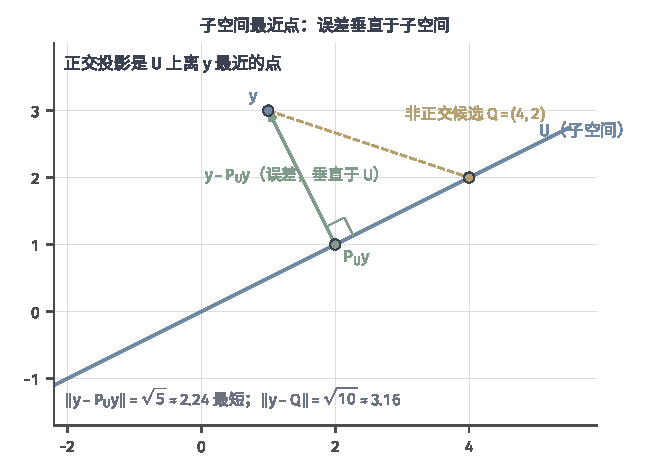
\includegraphics[width=112mm]{figures/00-shared/mathematical-preliminaries-upper/02-linear-spaces/matplotlib/ls-orthogonal-projection-nearest/ls-orthogonal-projection-nearest.pdf}
  \caption{直线子空间$U$（过原点、方向$(2,1)$）上离$\bm y=(1,3)^\top$最近的点是正交投影
  $\bm p=(2,1)^\top$，误差$\bm y-\bm p=(-1,2)^\top$与$U$垂直（直角小方块）；
  同一线上的另一候选$\bm q=(4,2)^\top$到$\bm y$的距离$\sqrt{10}$明显大于最短距离$\sqrt5$。
  这是解析式教学构造。}
  \label{fig:ls-orthogonal-projection-nearest}
\end{figure}

\paragraph{正规方程}

回到矩阵$\bm A$，取$U=\operatorname{range}(\bm A)$，设最近点是$\hat{\bm b}=\bm A\hat{\bm x}$。
列空间由$\bm A$的各列张成，残差$\bm r=\bm b-\bm A\hat{\bm x}$与列空间正交，就是与每一列$\bm a_j$正交，
即$\bm a_j^\top\bm r=0$，$j=1,\ldots,d$，合写为$\bm A^\top\bm r=\bm0$。代入$\bm r$得到\term{正规方程}（normal equations）
\begin{equation}
\begin{gathered}
\bm A^\top(\bm b-\bm A\hat{\bm x})=\bm0\\
\bm A^\top\bm A\hat{\bm x}=\bm A^\top\bm b.
\end{gathered}
\label{eq:linear-algebra-normal-equations}
\end{equation}
“正规”指法向，即残差与列空间正交，不是归一化。由定理~\ref{thm:ls-four-subspaces-orthogonality}，
这也就是说残差落在左零空间$\operatorname{null}(\bm A^\top)$中：最小二乘把$\bm b$分成可达的部分与完全不可达的部分。
下面用一个三个方程、两个未知量的例子计算正规方程。

\begin{example}[超定方程的最小二乘解]
\label{ex:ls-normal-equations-three-by-two}
取$\bm A=\left[\begin{smallmatrix}1&0\\0&1\\1&1\end{smallmatrix}\right]$、$\bm b=(2,3,2)^\top$。
列空间中的向量形如$(x_1,x_2,x_1+x_2)^\top$，第三坐标等于前两坐标之和；而$\bm b$的第三坐标$2\neq2+3$，
所以$\bm b$不在列空间中，方程$\bm A\bm x=\bm b$无解。计算
\[
\begin{gathered}
\bm A^\top\bm A=\begin{bmatrix}2&1\\1&2\end{bmatrix}\\
\bm A^\top\bm b=\begin{bmatrix}4\\5\end{bmatrix},
\end{gathered}
\]
解正规方程$2\hat x_1+\hat x_2=4$、$\hat x_1+2\hat x_2=5$，得$\hat{\bm x}=(1,2)^\top$。
最近点为$\bm A\hat{\bm x}=(1,2,3)^\top$，残差为$\bm r=\bm b-\bm A\hat{\bm x}=(1,1,-1)^\top$；
它与两列$(1,0,1)^\top$、$(0,1,1)^\top$的内积都是零，满足正交性判据。
\end{example}

图~\ref{fig:ls-least-squares-residual}画出这个例子。

\begin{figure}[htbp]
  \centering
  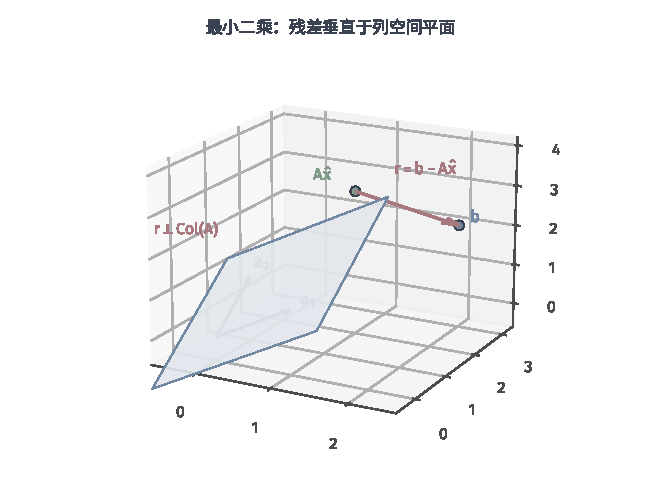
\includegraphics[width=112mm]{figures/00-shared/mathematical-preliminaries-upper/02-linear-spaces/matplotlib/ls-least-squares-residual/ls-least-squares-residual.pdf}
  \caption{列空间平面上的最近点。$\bm A=\left[\begin{smallmatrix}1&0\\0&1\\1&1\end{smallmatrix}\right]$，
  列$\bm a_1=(1,0,1)^\top$、$\bm a_2=(0,1,1)^\top$张成浅蓝平面；$\bm b=(2,3,2)^\top$，
  最近拟合值$\bm A\hat{\bm x}=(1,2,3)^\top$，残差$\bm r=(1,1,-1)^\top$满足
  $\bm r^\top\bm a_1=\bm r^\top\bm a_2=0$。透视教学构造。}
  \label{fig:ls-least-squares-residual}
\end{figure}

正规方程是由几何判据推出的；也可以直接验证，它的解确实使目标取全局最小。

设$\hat{\bm x}$满足正规方程，
$\bm r=\bm b-\bm A\hat{\bm x}$，对任意增量$\bm h$，$\bm A(\hat{\bm x}+\bm h)-\bm b=\bm A\bm h-\bm r$，展开平方长度得
\[
 \lVert\bm A(\hat{\bm x}+\bm h)-\bm b\rVert_2^2
 =\lVert\bm r\rVert_2^2-2(\bm A\bm h)^\top\bm r+\lVert\bm A\bm h\rVert_2^2
 =\lVert\bm r\rVert_2^2-2\bm h^\top(\bm A^\top\bm r)+\lVert\bm A\bm h\rVert_2^2 .
\]
正规方程使中间项为零，剩下的$\lVert\bm A\bm h\rVert_2^2\geq0$，所以任何移动都不会减小目标。
反之，若$\hat{\bm x}$是最小点，则拟合值$\bm A\hat{\bm x}$是列空间中离$\bm b$最近的点，由正交性判据，
残差与列空间正交，$\hat{\bm x}$满足正规方程。于是最小二乘问题与正规方程同解，
求最小点就是解这个$d$阶对称线性方程。

用一般子空间的基矩阵$\bm B$代替$\bm A$，并在一般内积下把$\bm B^\top\bm B$的元素换成内积，正规方程成为
\begin{equation}
\begin{gathered}
\bm G\bm c=\bigl(\langle\bm b_i,\bm y\rangle\bigr)_{i=1}^r\\
g_{i,j}=\langle\bm b_i,\bm b_j\rangle,
\end{gathered}
\label{eq:ls-gram-system}
\end{equation}
系数矩阵$\bm G$是基向量的Gram矩阵；逐行写就是$\sum_j\langle\bm b_i,\bm b_j\rangle c_j=\langle\bm b_i,\bm y\rangle$，
即残差$\bm y-\sum_jc_j\bm b_j$与每个基向量正交。这就把问题~\eqref{eq:ls-nearest-point-coefficients}化成了线性方程。

在示例~\ref{ex:ls-nonorthogonal-coefficients}中，$\bm G=\left[\begin{smallmatrix}2&1\\1&1\end{smallmatrix}\right]$，右端为$(1,0)^\top$，
解得$\bm c=(1,-1)^\top$，与直接观察一致。这里两个基向量张成整个平面，所以最近点就是$\bm y$本身；
Gram系统的作用是把内积$(1,0)^\top$纠正为真正的系数。

基向量标准正交时，Gram矩阵是单位矩阵，Gram系统不必求解：系数就是内积，最近点直接写出，
\[
 \bm p=\sum_j\langle\bm q_j,\bm y\rangle\bm q_j .
\]
这就是第~\ref{chap:normed-inner-product-spaces}章的正交分解公式~\eqref{eq:ls-orthonormal-projection}，每个系数只与自己的方向有关，互不干扰。
它是第~\ref{sec:ls-qr-method}节用QR分解解最小二乘的出发点。

\subsection{解的存在与唯一性}
\label{sec:ls-ls-existence}

最近点$\hat{\bm b}$作为列空间中的点总是存在且唯一，但正规方程的未知量是产生它的输入$\hat{\bm x}$。
本部分回答：这样的输入是否总存在，是否唯一，不唯一时全部解是什么样子，唯一时系数是否可靠。

\paragraph{存在性}

正规方程对任意$\bm b$都有解。几何上这很自然：$\hat{\bm b}$在列空间中，总有输入产生它，而这个输入满足正规方程。
也可以从方程本身验证。先看系数矩阵的零空间：若$\bm A^\top\bm A\bm x=\bm0$，则
$\lVert\bm A\bm x\rVert_2^2=\bm x^\top\bm A^\top\bm A\bm x=0$，即$\bm A\bm x=\bm0$；反向包含显然。故
\begin{equation}
 \ker(\bm A^\top\bm A)=\ker\bm A.
 \label{eq:ls-normal-kernel}
\end{equation}
由定理~\ref{thm:ls-four-subspaces-orthogonality}，对任意矩阵有$\operatorname{range}(\bm A^\top)=(\ker\bm A)^\perp$。把它用在对称矩阵$\bm A^\top\bm A$上，得
$\operatorname{range}(\bm A^\top\bm A)=\ker(\bm A^\top\bm A)^\perp=(\ker\bm A)^\perp=\operatorname{range}(\bm A^\top)$。
右端$\bm A^\top\bm b$显然在$\operatorname{range}(\bm A^\top)$中，所以方程总是相容。

\paragraph{全部解与唯一性}

拟合值唯一，不代表输入唯一。正规方程是相容的线性方程，按第~\ref{sec:ls-uniqueness-freedom}节的结论，它的全部解是一个解加上系数矩阵的零空间；
由~\eqref{eq:ls-normal-kernel}，全部解为
\begin{equation}
 \hat{\bm x}+\ker\bm A.
 \label{eq:ls-all-ordinary-solutions}
\end{equation}
这些解给出同一个拟合值，因为零空间方向不改变输出。于是解唯一当且仅当$\bm A$满列秩。
此时$\bm A^\top\bm A$正定（$\bm x\neq\bm0$时$\bm x^\top\bm A^\top\bm A\bm x=\lVert\bm A\bm x\rVert_2^2>0$），因而可逆，唯一解为
\begin{equation}
 \hat{\bm x}=(\bm A^\top\bm A)^{-1}\bm A^\top\bm b.
 \label{eq:linear-algebra-full-rank-least-squares}
\end{equation}
用子空间的基表示时同样如此：基向量线性无关，Gram矩阵$\bm G$正定，Gram系统~\eqref{eq:ls-gram-system}的解唯一。

这里有两层唯一性要分清。最近点作为$U$中的点总是唯一的；它的系数只在张成向量线性无关时唯一：
若$\bm B\bm c_1=\bm B\bm c_2$，则$\bm B(\bm c_1-\bm c_2)=\bm0$，线性无关迫使$\bm c_1=\bm c_2$。

秩亏时，例如$\bm A$有两列相同，正规方程相容但有无穷多解，第~\ref{sec:ls-select-among-solutions}节的讨论原样适用：
若要求欧氏范数最小，就去掉不改变输出的零空间分量，所得的解落在$(\ker\bm A)^\perp$中，
它也是相容方程$\bm A\bm x=\hat{\bm b}$的最小范数解。
在任意秩下把这一选择写成矩阵需要伪逆，见第~\ref{sec:ls-pseudoinverse}节。

无论解是否唯一，最小值都只由正交分解决定。$\hat{\bm b}\perp\bm r$，勾股恒等式给出
$\lVert\bm b\rVert_2^2=\lVert\hat{\bm b}\rVert_2^2+\lVert\bm r\rVert_2^2$：
观测的平方长度分成被列空间解释的部分与残差部分，最小平方残差
$\lVert\bm r\rVert_2^2=\lVert\bm b\rVert_2^2-\lVert\hat{\bm b}\rVert_2^2$对全部解相同。
示例~\ref{ex:ls-normal-equations-three-by-two}中，$\lVert\bm b\rVert_2^2=17$，$\lVert\hat{\bm b}\rVert_2^2=1+4+9=14$，$\lVert\bm r\rVert_2^2=3$。

\paragraph{唯一不等于稳定}

满列秩只保证系数唯一，不保证系数可靠。下面的例子中，设计矩阵的两列接近共线。

\begin{example}[近共线设计：唯一但不稳定的系数]
\label{ex:ls-nearly-collinear-design}
取互相正交的向量$\bm c_1=(1,1,1)^\top$与$\bm q=(0,1,-1)^\top$。
设计矩阵$\bm X_\varepsilon$的两列为$\bm c_1$与$\bm c_1+\varepsilon\bm q$，响应为$\bm y=\bm c_1+\delta\bm q$。
利用$\bm c_1^\top\bm q=0$、$\lVert\bm c_1\rVert_2^2=3$、$\lVert\bm q\rVert_2^2=2$，正规方程为
\[
 \begin{bmatrix}3&3\\3&3+2\varepsilon^2\end{bmatrix}\hat{\bm w}
 =\begin{bmatrix}3\\3+2\varepsilon\delta\end{bmatrix},
\]
系数矩阵的行列式为$6\varepsilon^2$。$\varepsilon\neq0$时满列秩，解为
\begin{equation}
\begin{gathered}
\hat{\bm w}_\varepsilon
 =\begin{bmatrix}1-\delta/\varepsilon\\\delta/\varepsilon\end{bmatrix}\\
\bm X_\varepsilon\hat{\bm w}_\varepsilon=\bm y,
\end{gathered}
\label{eq:linear-algebra-nearly-collinear-least-squares}
\end{equation}
后一式可直接验证：$(1-\delta/\varepsilon)\bm c_1+(\delta/\varepsilon)(\bm c_1+\varepsilon\bm q)=\bm c_1+\delta\bm q$。
取$\varepsilon=0.01$、$\delta=0.1$，系数为$(-9,10)^\top$，残差却为零。

$\varepsilon=0$时两列重合为$\bm c_1$。此时$\bm y=\bm c_1+\delta\bm q$本身就是正交分解，最近输出为$\bm c_1$，
残差为$\delta\bm q$，平方残差为$2\delta^2$；满足$w_1+w_2=1$的系数都是解。
\end{example}

所以$\delta\neq0$时，随着$\varepsilon\to0$，精确拟合所需的系数趋于无穷，而极限矩阵已经不能精确拟合。
拟合值可以相当稳定，表示它的两个系数却可能很大，而且对$\varepsilon$、$\delta$极为敏感。
这是近共线几何本身的性质，不是计算机舍入造成的；它的定量刻画见第~\ref{sec:ls-ordinary-ls-sensitivity}节。

\subsection{正规方程法}
\label{sec:ls-normal-equations-method}

本小节的输入仍是$\bm A\in\mathbb R^{m\times d}$与$\bm b\in\mathbb R^m$，这里假设$m\geq d$且$\bm A$满列秩。原方程可能不相容，因此输出改为唯一的最小二乘解$\hat{\bm x}$。

上一小节已经把最优性写成$\bm A^\top(\bm b-\bm A\hat{\bm x})=0$；正规方程法直接把这个条件当作待求解的$d$阶正定方程。

最直接的算法是解正规方程。$\bm A$满列秩时$\bm A^\top\bm A$对称正定，可以用Cholesky分解：
先形成$\bm A^\top\bm A$与$\bm A^\top\bm b$，分解$\bm A^\top\bm A=\bm L\bm L^\top$，再依次前代解$\bm L\bm z=\bm A^\top\bm b$、
回代解$\bm L^\top\hat{\bm x}=\bm z$。加权问题对$\bm A^\top\bm M\bm A$作同样的分解。
稠密情形下，形成$\bm A^\top\bm A$约需$md^2$次乘法，分解约需$d^3/3$次运算，多个右端复用同一分解。
$m$远大于$d$且矩阵条件良好时，形成正规矩阵再作Cholesky分解，通常比稠密QR所需运算更少。

例如仍用$\bm A=\left[\begin{smallmatrix}1&0\\0&1\\1&1\end{smallmatrix}\right]$和$\bm b=(2,3,2)^\top$。先算出
\[
 \bm G=\bm A^\top\bm A=\begin{bmatrix}2&1\\1&2\end{bmatrix},\qquad
 \bm c=\bm A^\top\bm b=\begin{bmatrix}4\\5\end{bmatrix}.
\]
Cholesky因子为$\bm L=\left[\begin{smallmatrix}\sqrt2&0\\1/\sqrt2&\sqrt{3/2}\end{smallmatrix}\right]$。前代$\bm L\bm z=\bm c$得到$\bm z=(2\sqrt2,\sqrt6)^\top$，回代$\bm L^\top\hat{\bm x}=\bm z$得到$\hat{\bm x}=(1,2)^\top$。原残差为$(1,1,-1)^\top$，虽非零，却满足$\bm A^\top\bm r=0$，这才是最小二乘计算要核验的条件。

形成$\bm A^\top\bm A$会损失精度。由第~\ref{sec:ls-svd}节的奇异值分解，$\bm A^\top\bm A$的特征值是$\bm A$的奇异值的平方：
$\bm A$中被压缩得很厉害的方向，在$\bm A^\top\bm A$中被压缩两次，就像一个小数取平方后更小；
浮点计算中，这种方向可能与零无法区分。所以正规方程法只在各列明显线性无关、
$\bm A^\top\bm A$的正定性有充足余量时可靠。秩亏时唯一性本身就不成立；近秩亏时，如示例~\ref{ex:ls-nearly-collinear-design}，
系数本来就不稳定，Cholesky分解成功也不说明结果可用。这种平方造成的精度损失在第~\ref{sec:ls-numerical-sensitivity}节用条件数定量估计。

\subsection{QR分解}
\label{sec:ls-qr-method}
\label{sec:linear-algebra-direct-residual}

另一条路线不形成$\bm A^\top\bm A$，而是先给列空间换一组标准正交基。
第~\ref{chap:normed-inner-product-spaces}章的Gram--Schmidt正交化正是做这件事，它把满列秩矩阵写成经济型QR分解
$\bm A=\bm Q\bm R$（式~\eqref{eq:ls-qr-factorization}），$\bm Q$的列是列空间的标准正交基，$\bm R$是对角元为正的上三角矩阵。
QR适合最小二乘的根本原因是：正交矩阵保持欧氏长度，用它变换残差，只改坐标，不改长度，最小点也就不变。

设$\bm A$满列秩，把$\bm Q$的列扩充成$\mathbb R^m$的标准正交基，得到完全QR分解
$\bm A=[\bm Q_1\;\bm Q_2]\left[\begin{smallmatrix}\bm R\\\bm0\end{smallmatrix}\right]=\bm Q_1\bm R$，
其中$[\bm Q_1\;\bm Q_2]$是$m$阶正交矩阵，$\bm Q_1$有$d$列，就是经济型分解中的$\bm Q$；$\bm Q_2$的列张成列空间的正交补。
记$\bm c_1=\bm Q_1^\top\bm b$、$\bm c_2=\bm Q_2^\top\bm b$。用$[\bm Q_1\;\bm Q_2]^\top$变换残差，
\[
 \lVert\bm A\bm x-\bm b\rVert_2^2
 =\left\lVert\begin{bmatrix}\bm R\bm x-\bm c_1\\-\bm c_2\end{bmatrix}\right\rVert_2^2
 =\lVert\bm R\bm x-\bm c_1\rVert_2^2+\lVert\bm c_2\rVert_2^2 .
\]
第二项与$\bm x$无关，是无法消除的残差；第一项可以通过解上三角方程$\bm R\hat{\bm x}=\bm c_1$降为零。
满列秩时$\bm R$的对角元非零，回代即得唯一解，最小平方残差就是$\lVert\bm c_2\rVert_2^2=\lVert\bm b\rVert_2^2-\lVert\bm c_1\rVert_2^2$，
所以$\bm Q_2$不必形成。整个过程不出现$\bm A^\top\bm A$，避免了正规方程法的平方尺度损失，
代价是分解的运算量高于Cholesky。

下面用QR分解重算示例~\ref{ex:ls-normal-equations-three-by-two}。

\begin{example}[用QR分解求解最小二乘]
\label{ex:ls-qr-three-by-two}
仍取$\bm A=\left[\begin{smallmatrix}1&0\\0&1\\1&1\end{smallmatrix}\right]$、$\bm b=(2,3,2)^\top$。
Gram--Schmidt先给出$\bm q_1=(1,0,1)^\top/\sqrt2$。$\bm a_2$在$\bm q_1$上的分量为$r_{1,2}=\bm q_1^\top\bm a_2=1/\sqrt2$，扣除后
\[
 \begin{gathered}
\bm v_2=(0,1,1)^\top-\tfrac12(1,0,1)^\top=(-\tfrac12,1,\tfrac12)^\top\\
r_{2,2}=\lVert\bm v_2\rVert_2=\sqrt{3/2},
 \end{gathered}
\]
再令$\bm q_2=\bm v_2/r_{2,2}$。于是
\[
\begin{gathered}
\bm R=\begin{bmatrix}\sqrt2&1/\sqrt2\\0&\sqrt{3/2}\end{bmatrix}\\
\bm c_1=\begin{bmatrix}\bm q_1^\top\bm b\\\bm q_2^\top\bm b\end{bmatrix}=\begin{bmatrix}2\sqrt2\\\sqrt6\end{bmatrix}.
\end{gathered}
\]
回代解$\bm R\hat{\bm x}=\bm c_1$，得$\hat x_2=\sqrt6/\sqrt{3/2}=2$、$\hat x_1=(2\sqrt2-2/\sqrt2)/\sqrt2=1$，
与正规方程的结果相同。最小平方残差为$\lVert\bm b\rVert_2^2-\lVert\bm c_1\rVert_2^2=17-(8+6)=3$，也与前面一致。
\end{example}

同一分解还给出最近点。最近点为$\hat{\bm b}=\bm A\hat{\bm x}=\bm Q_1\bm R\hat{\bm x}=\bm Q_1\bm c_1=\bm Q_1\bm Q_1^\top\bm b$，
$\bm c_1$的分量就是$\bm b$在各正交方向上的坐标，不必另解Gram系统。

它也判定相容性：$\bm c_2=\bm0$当且仅当$\bm b$在列空间中，
此时回代得到的就是原方程的精确解；$\bm c_2\neq\bm0$时原方程不相容，$\lVert\bm c_2\rVert_2$就是$\bm b$到列空间的距离。
例如$\bm A=\left[\begin{smallmatrix}1&1\\1&0\\0&1\end{smallmatrix}\right]$、$\bm b=(2,1,1)^\top=\bm A(1,1)^\top$时$\bm c_2=\bm0$，
回代得到精确解$\hat{\bm x}=(1,1)^\top$。这就是第~\ref{sec:ls-direct-methods}节所说的：
超定而满列秩的方程，相容性的判断与唯一解的计算可以由同一个QR分解一次完成。

$\bm A$秩亏时，Gram--Schmidt在某一列得不到新方向，$\bm R$不再可逆，上面的回代不能直接进行；
这时最小二乘解不唯一，最小范数解由第~\ref{sec:ls-pseudoinverse}节的伪逆给出。
有限精度下怎样借带列主元的QR判断秩，见第~\ref{sec:ls-orthogonalization-qr}节。

\paragraph{列空间投影与正规方程}

不做正交化，也可以从正规方程写出投影矩阵。$\bm A$满列秩时，最近点为
$\hat{\bm b}=\bm A\hat{\bm x}=\bm A(\bm A^\top\bm A)^{-1}\bm A^\top\bm b$，故
\begin{equation}
 \bm P_{\operatorname{range}(\bm A)}=\bm A(\bm A^\top\bm A)^{-1}\bm A^\top.
 \label{eq:ls-column-space-projector}
\end{equation}
直接相乘可验它对称且幂等。代入$\bm A=\bm Q\bm R$，得$\bm Q\bm R(\bm R^\top\bm R)^{-1}\bm R^\top\bm Q^\top=\bm Q\bm Q^\top$，
与式~\eqref{eq:linear-algebra-orthogonal-projector}一致，说明投影只取决于列空间，与所用的基无关。

回归中这个矩阵常称帽子矩阵，它把观测$\bm y$映成拟合值$\hat{\bm y}$；$\bm I-\bm P$则把观测映成残差，
它是到$\operatorname{range}(\bm A)^\perp=\operatorname{null}(\bm A^\top)$的正交投影。
加权内积下，同样的推导给出$\bm A(\bm A^\top\bm M\bm A)^{-1}\bm A^\top\bm M$；它幂等但一般不对称，
在普通内积下是斜投影，在$\bm M$内积下才是正交投影。

两个正交投影相乘一般不可交换，$\bm P_U\bm P_V\neq\bm P_V\bm P_U$，乘积也未必还是投影。
两者可交换时，乘积既幂等又对称，因而是到其像的正交投影。它的像含于$U$（左因子是$\bm P_U$），
也含于$V$（交换次序后左因子是$\bm P_V$），而$U\cap V$中的向量被它保持不变，所以它是到$U\cap V$的正交投影。


\subsection{修正Gram--Schmidt正交化}

上面已经说明如何用QR分解把最小二乘化为三角方程，现在还需说明分解本身怎样计算。
第~\ref{chap:normed-inner-product-spaces}章用Gram--Schmidt正交化构造它，那里假定精确算术：
式~\eqref{eq:ls-gram-schmidt}一次性减去$\bm a_j$在全部旧方向上的分量，每个系数都用原始的$\bm a_j$计算。

\term{修正Gram--Schmidt}（modified Gram--Schmidt）改为逐个扣除：先令$\bm u\leftarrow\bm a_j$，对$i=1,\ldots,j-1$依次计算$r_{i,j}=\langle\bm u,\bm q_i\rangle$并更新$\bm u\leftarrow\bm u-r_{i,j}\bm q_i$，最后归一化。

具体说，第$j$列处理结束后，令$r_{j,j}=\|\bm u\|_2$、$\bm q_j=\bm u/r_{j,j}$；若该范数为零，当前列不能提供新方向，应转入秩亏处理。对$j=1,\ldots,d$重复，输出$\bm Q=[\bm q_1\;\cdots\;\bm q_d]$与$\bm R=(r_{i,j})$。

随后计算$c_j=\bm q_j^\top\bm b$并回代$\bm R\hat{\bm x}=\bm c$，才完成输入$(\bm A,\bm b)$到最小二乘解的过程。前面的三行两列算例中，第二列只有一个旧方向可扣除，按这一流程同样得到$\hat{\bm x}=(1,2)^\top$。

精确算术中两种做法给出同样的结果：扣除第$i$个方向时，此前已减去的都是$\bm q_1,\ldots,\bm q_{i-1}$的倍数，它们与$\bm q_i$正交，所以$\langle\bm u,\bm q_i\rangle=\langle\bm a_j,\bm q_i\rangle$。

有限精度下，修正的做法每次都从已经扣除过的最新残差出发，算出的$\bm q_j$之间正交性的损失通常更小；
它的损失大致与$\kappa_2(\bm A)$乘单位舍入$u$同量级，原始做法则可能严重得多\scite{math-golub2013matrix}。
列之间越接近线性相关，扣除后剩下的$\bm u_j$越短，舍入误差在其中所占的比例越大，两种做法的差别也越明显。

同样的原因使列相关时的处理不能照搬精确算术：有限精度下$\bm u_j$很少恰好为零，判断“没有新方向”时要把$\lVert\bm u_j\rVert$与一个容限比较，
这正是第~\ref{sec:ls-ordinary-ls-sensitivity}节的数值秩问题。修正Gram--Schmidt的正交性损失仍随条件数增长；
需要$\bm Q$在工作精度下正交时，改用后面的Householder反射。

\subsection{Householder反射}
\label{sec:ls-orthogonalization-qr}

修正Gram--Schmidt仍从列出发构造$\bm Q$，列越接近线性相关，正交性损失越大，而这恰是最需要QR的情形。
稠密计算中更常用的做法反过来：用一串正交矩阵从左边作用于$\bm A$，逐列把主对角线以下的元素消成零，最后剩下上三角的$\bm R$。
正交矩阵保持长度，这样的消元不会放大误差，各步正交矩阵的乘积自然是正交的。
完成这一步的基本工具是\term{Householder反射}，它一次消去一列中主对角线以下的全部元素。

对非零向量$\bm a$，要找一个正交矩阵把它变成$\bm e_1$的倍数。由于正交变换保持长度，目标只能是$\pm\lVert\bm a\rVert_2\bm e_1$。
取$s=1$（若$a_1\geq0$）或$s=-1$（若$a_1<0$），令
\begin{equation}
\begin{gathered}
\bm v=\bm a+s\lVert\bm a\rVert_2\bm e_1\\
\bm H=\bm I-2\frac{\bm v\bm v^\top}{\bm v^\top\bm v}.
\end{gathered}
\label{eq:ls-householder}
\end{equation}
$\bm H$把$\bm v$方向的分量变号，与$\bm v$正交的分量保持不变，即关于以$\bm v$为法向的超平面作镜面反射；
它对称，且$\bm H^\top\bm H=\bm H^2=\bm I$，反射两次回到原处。

下面验证它把$\bm a$送到$\bm e_1$方向。记$\alpha=\lVert\bm a\rVert_2$，则
$\bm v^\top\bm a=\alpha^2+s\alpha a_1$，$\bm v^\top\bm v=\alpha^2+2s\alpha a_1+\alpha^2=2\bm v^\top\bm a$，于是
\[
 \bm H\bm a=\bm a-2\frac{\bm v^\top\bm a}{\bm v^\top\bm v}\bm v=\bm a-\bm v=-s\alpha\bm e_1 .
\]
符号$s$取与$a_1$相同，是为了让$\bm v$的首元素$a_1+s\alpha$是两个同号数相加，避免两个相近的数相减而丢失有效数字。
应用$\bm H$时只需保存$\bm v$，计算$\bm H\bm x=\bm x-2\bm v(\bm v^\top\bm x)/(\bm v^\top\bm v)$，不必形成整个矩阵。

\begin{example}[二维向量的Householder反射]
\label{ex:ls-householder-two-dim}
取$\bm a=(3,4)^\top$。$a_1>0$，取$s=1$；$\alpha=5$，$\bm v=\bm a+5\bm e_1=(8,4)^\top$，$\bm v^\top\bm v=80$。于是
\[
 \bm H=\bm I-\frac{2}{80}\bm v\bm v^\top
 =\bm I-\frac1{40}\begin{bmatrix}64&32\\32&16\end{bmatrix}
 =\begin{bmatrix}-3/5&-4/5\\-4/5&3/5\end{bmatrix},
\]
$\bm H\bm a=(-5,0)^\top$，与$-s\alpha\bm e_1=-5\bm e_1$一致。
\end{example}

对矩阵做QR时，第$k$步对第$k$列从第$k$个元素往下的部分构造反射，
只作用于尚未处理的右下子块。$d$步之后，$\bm H_d\cdots\bm H_1\bm A=\left[\begin{smallmatrix}\bm R\\\bm0\end{smallmatrix}\right]$，
各反射的乘积的转置就是完全QR分解中的$[\bm Q_1\;\bm Q_2]$；
$\bm R$的对角元可能为负，把相应的行与$\bm Q_1$的列同时变号即可化为对角元为正的形式。

把这一过程用于求解时，令工作矩阵$\bm F=\bm A$、工作右端$\bm c=\bm b$。第$k$步用$\bm F_{k:m,k}$构造反射，把它同时作用于$\bm F_{k:m,k:d}$与$\bm c_{k:m}$；前面已经消出的零不再改变。全部列处理完后，$\bm F$的前$d$行是$\bm R$，$\bm c$的前$d$项是$\bm c_1$，回代得到$\hat{\bm x}$，其余项组成不可消除的残差坐标$\bm c_2$。

若为统一符号而翻转$\bm R$某行，也须同步翻转$\bm c_1$的对应项。

例如取$\bm A=\left[\begin{smallmatrix}3&1\\4&2\end{smallmatrix}\right]$、$\bm b=(4,6)^\top$。用上例的反射同时变换二者，得到
\[
 \bm H\bm A=\begin{bmatrix}-5&-11/5\\0&2/5\end{bmatrix},\qquad
 \bm H\bm b=\begin{bmatrix}-36/5\\2/5\end{bmatrix}.
\]
由第二行得$x_2=1$，再由第一行得$x_1=1$。反射后的矩阵已经是上三角形，因而本例无需继续消元；代回可验$\bm A\bm x=\bm b$。

稠密$m\times d$矩阵的Householder QR约需$2md^2-2d^3/3$次浮点运算。$\bm Q$不必显式形成，
保存各步的反射向量即可；求解最小二乘时，把同样的反射依次作用于$\bm b$就得到$\bm c_1$与$\bm c_2$，
多个右端复用全部反射与$\bm R$。岭回归对堆叠矩阵~\eqref{eq:ls-augmented-system}作同样的分解即可，
不必形成$\bm A^\top\bm A+\lambda\bm L^\top\bm L$。

秩亏或接近秩亏时，要先把列重新排序。带列主元的QR在每一步选剩余部分中最长的一列先处理，
使接近零的对角元集中在$\bm R$的尾部，从而暴露数值秩，阈值按数据误差的尺度选取，这比计算奇异值分解便宜。
若精确秩为$r$，只用前$r$个主元列回代、其余未知量取零，得到的基本解使原目标达到最小，
但一般不是最小范数解，正如第~\ref{sec:ls-select-among-solutions}节中自由变量取零得到的特解一般不是最小范数解。若$r$由数值阈值确定，被忽略的方向未必精确为零，此时得到的是截断近似，不能保证它是原问题的精确最小二乘解。

\subsection{Givens旋转}

Householder一次处理整段列向量；当只需消去少数元素，或者新观测只增加了一行时，重新反射整个子块可能不划算。Givens方法只混合两行，同步更新这两行的系数与右端，仍以得到三角方程并回代为目标。输入输出与Householder求解相同，差别在于每一步消元的范围。

\term{Givens旋转}一次只消去一个元素。它在第$i$、$j$两个坐标构成的平面内作旋转，其余坐标不变；
在这两个坐标上的作用是
\begin{equation}
\begin{gathered}
\begin{bmatrix}a_i\\a_j\end{bmatrix}\mapsto
 \begin{bmatrix}c&s\\-s&c\end{bmatrix}
 \begin{bmatrix}a_i\\a_j\end{bmatrix}\\
c^2+s^2=1.
\end{gathered}
\label{eq:ls-givens}
\end{equation}
这里的$c$、$s$是旋转角的余弦与正弦，与Householder反射中的符号$s$无关。
完整的矩阵$\bm G(i,j)$是在单位矩阵的$(i,i),(i,j),(j,i),(j,j)$四个位置放上$c,s,-s,c$。
为了消去$a_j$，取$r=\sqrt{a_i^2+a_j^2}$，$c=a_i/r$、$s=a_j/r$，则新分量为
$(ca_i+sa_j,\,-sa_i+ca_j)=(r,0)$。$r=0$时两个分量本已为零，无需旋转。

\begin{example}[二维向量的Givens旋转]
\label{ex:ls-givens-two-dim}
取$(a_i,a_j)=(3,4)$。$r=\sqrt{9+16}=5$，$c=3/5$、$s=4/5$，旋转后
\[
 \begin{gathered}
ca_i+sa_j=\frac95+\frac{16}5=5\\
-sa_i+ca_j=-\frac{12}5+\frac{12}5=0 ,
 \end{gathered}
\]
第二个分量被消去，长度$5$全部转到第一个分量上。
\end{example}

对一般$m\times d$的输入，先令$\bm F=\bm A$、$\bm c=\bm b$。按列$k=1,\ldots,d$处理，每列从底部$i=m$向上到$k+1$，对当前的$f_{i-1,k},f_{i,k}$构造旋转，混合第$i-1,i$行的第$k$至$d$列，并同步混合$c_{i-1},c_i$。这样逐个把对角线以下的元素消为零，而且不会破坏前面列中的零。最后取前$d$行得到$\bm R$，回代$\bm R\hat{\bm x}=\bm c_{1:d}$。

在上一小节同一个二阶方程中，旋转矩阵取$\bm G=\left[\begin{smallmatrix}3/5&4/5\\-4/5&3/5\end{smallmatrix}\right]$，得到$\bm G\bm A=\left[\begin{smallmatrix}5&11/5\\0&2/5\end{smallmatrix}\right]$与$\bm G\bm b=(36/5,2/5)^\top$。回代仍得$(1,1)^\top$。两种正交变换的中间符号不同，最终求解的是同一个原方程。

Givens每次只改动两行，适合稀疏或带状矩阵，也适合在最小二乘中新增一条观测时逐步更新已有的QR；
对稠密矩阵，它消去同样多的元素需要更多运算，不如Householder。
图~\ref{fig:ls-givens-householder-elimination}把两种变换并置。图中的反射取另一种符号，
把向量映到$(r,0)^\top$而不是$(-r,0)^\top$，精确算术中两种选择都可以。

\begin{figure*}[htbp]
  \centering
  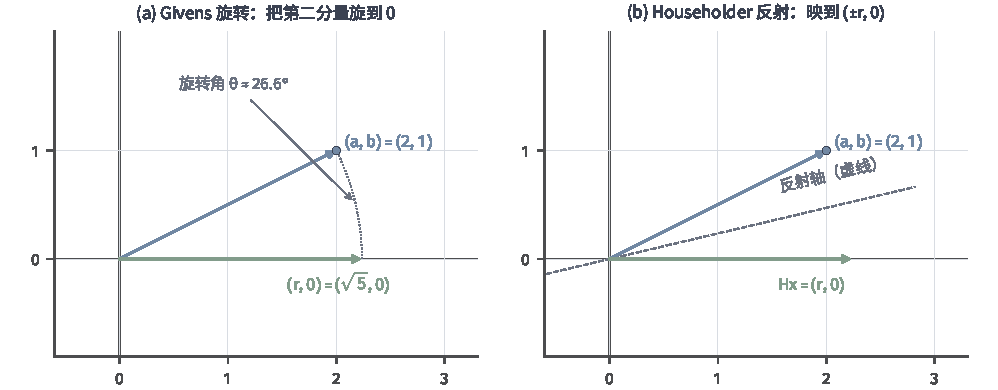
\includegraphics[width=168.998mm]{figures/00-shared/mathematical-preliminaries-upper/02-linear-spaces/matplotlib/ls-givens-householder-elimination/ls-givens-householder-elimination.pdf}
  \caption{两种初等正交消元。左：Givens旋转把$(a,b)=(2,1)^\top$沿圆弧旋到
  $(r,0)^\top$，$r=\sqrt5$，旋转角$\theta=\arctan(1/2)$；右：Householder反射沿角平分线
  把同一向量映到$(r,0)^\top$。两者都是正交变换，保持长度，区别在旋转（行列式$+1$）与
  反射（对称正交）。解析式教学构造。}
  \label{fig:ls-givens-householder-elimination}
\end{figure*}

至此，正规方程与QR都给出了完整的直接求解过程：前者形成正定系统，后者把系数和右端一起作正交变换，再解三角方程。当矩阵很大、无法方便地保存这些因子时，下一组方法用矩阵向量乘法逐步构造小问题。
% LSMR recursion checked against Fong and Saunders, SIAM J. Sci. Comput. 33 (2011), Algorithm LSMR.
% Extended Kaczmarz uses the synchronous old-z update of Zouzias and Freris, arXiv:1205.5770, Algorithm 3.
\subsection{Golub--Kahan双对角化}
\label{sec:ls-bidiagonal-iteration}

前面的QR方法适合能够保存分解结果的问题。若$\bm A\in\mathbb R^{m\times d}$很大，或者只能够计算$\bm A\bm v$与$\bm A^\top\bm u$，可以逐步构造低维问题，每一步只使用这两种乘法。下面从零初值说明；非零初值可以先以$\bm b-\bm A\bm x_0$为右端项求修正，但还要单独检查所得解的零空间分量。

以下统一输入$\bm A,\bm b$、两种残差的容差与最大步数，初值固定为$\bm x_0=0$。LSQR与LSMR的最终输出都是$d$维近似解，区别是每个子空间中优化哪一种残差。双对角化只是二者共享的准备过程：它输出基向量及双对角系数，还没有给出近似解。

为什么要交替使用$\bm A$与$\bm A^\top$？$\bm A$把$d$维未知量送入$m$维观测空间，而最优性条件$\bm A^\top\bm r=0$又把观测残差送回未知量空间。分别在两个空间中保持正交基，就能用很少的系数记录这两个作用，并把大问题的残差精确地表示成小问题的残差。

若$\bm b=0$，零向量已是最小范数解。否则令$\beta_1=\lVert\bm b\rVert_2$、$\bm u_1=\bm b/\beta_1$，再计算$\alpha_1=\lVert\bm A^\top\bm u_1\rVert_2$。若$\alpha_1=0$，零向量已满足正规方程。

当$\alpha_1>0$时令$\bm v_1=\bm A^\top\bm u_1/\alpha_1$。Golub--Kahan双对角化按下式交替生成两个空间中的向量：
\begin{align*}
 \bm p&=\bm A\bm v_k-\alpha_k\bm u_k,\\
 \beta_{k+1}&=\lVert\bm p\rVert_2,\\
 \bm u_{k+1}&=\bm p/\beta_{k+1},\\
 \bm q&=\bm A^\top\bm u_{k+1}-\beta_{k+1}\bm v_k,\\
 \alpha_{k+1}&=\lVert\bm q\rVert_2,\\
 \bm v_{k+1}&=\bm q/\alpha_{k+1}.
\end{align*}

待归一化向量为零时，不能执行对应除法。

若$\beta_{k+1}=0$，当前$\bm B_k$的最后一个下对角元已知为零；此时可令后续旋转所需的$\alpha_{k+1}=0$作为终止时的约定，不定义$\bm u_{k+1}$或$\bm v_{k+1}$。若$\beta_{k+1}>0$但$\alpha_{k+1}=0$，则已知$\bm B_k$和该零值，也不定义$\bm v_{k+1}$。

两种情形都先用已生成的系数完成当前小问题及$\bm x_k$的更新，再检查原残差和正规残差，不构造后续不存在的基向量。

减去旧方向的分量使所得向量在精确算术中与已有基正交。

当$\beta_{k+1}>0$时，把已生成的$\bm u_i$和$\bm v_i$分别排成列，得到$\bm A\bm V_k=\bm U_{k+1}\bm B_k$，其中$\bm B_k$的主对角为$\alpha_1,\ldots,\alpha_k$，下对角为$\beta_2,\ldots,\beta_{k+1}$。若$\beta_{k+1}=0$，则去掉$\bm B_k$的全零末行，记剩余方阵为$\widehat{\bm B}_k$，此时使用$\bm A\bm V_k=\bm U_k\widehat{\bm B}_k$，无需构造$\bm u_{k+1}$。

\subsection{LSQR算法}

有了双对角化输出，下一步要决定原变量怎样取值。LSQR把候选解限制在$\operatorname{span}\{\bm v_1,\ldots,\bm v_k\}$中，并在其中最小化原残差。也就是说，输入数据未变，只把每轮需要选择的未知量从$d$个原坐标换成$k$个子空间坐标。

选择$\bm x_k=\bm V_k\bm y$，并利用$\bm b=\beta_1\bm u_1$与已生成的$\bm U$的正交性，原残差范数化为$\lVert\beta_1\bm e_1-\bm B_k\bm y\rVert_2$。末行因$\beta_{k+1}=0$而删去时，改用$\widehat{\bm B}_k$及$k$维的$\bm e_1$，结果相同。LSQR在每一步求解这个小型最小二乘问题；因此精确算术下，随着候选空间扩大，原残差范数不增。实现可以用Givens旋转逐步更新小问题，不必每轮重新分解，也不必形成$\bm A^\top\bm A$。避免形成正规矩阵能减少填充及其形成误差，却不能消除原问题的小奇异值。

具体实现时，可将新一行双对角元素用一次平面旋转消去，并同时更新解。初始化$\bm x_0=\bm0$、$\bm w_1=\bm v_1$、$\bar\rho_1=\alpha_1$、$\bar\phi_1=\beta_1$。第$k$轮先做上述双对角化，再依次计算
\begin{align*}
 \rho_k&=\sqrt{\bar\rho_k^2+\beta_{k+1}^2},\\
 c_k&=\bar\rho_k/\rho_k,\\
 s_k&=\beta_{k+1}/\rho_k,\\
 \theta_{k+1}&=s_k\alpha_{k+1},\\
 \bar\rho_{k+1}&=-c_k\alpha_{k+1},\\
 \phi_k&=c_k\bar\phi_k,\quad \bar\phi_{k+1}=s_k\bar\phi_k,
\end{align*}
并更新$\bm x_k=\bm x_{k-1}+(\phi_k/\rho_k)\bm w_k$与$\bm w_{k+1}=\bm v_{k+1}-(\theta_{k+1}/\rho_k)\bm w_k$。这些标量记录逐次旋转，小问题的解通过方向$\bm w_k$累加到原变量中。

这个累加式可以从回代读出，而无需把它当作独立公式记忆。旋转把双对角小矩阵化为上双对角矩阵，当前对角元是$\rho_k$，与下一列的耦合是$\theta_{k+1}$。把三角求解与$\bm V_k\bm y$合在一起，已消去的耦合由$\bm w_{k+1}=\bm v_{k+1}-(\theta_{k+1}/\rho_k)\bm w_k$记录；当前右端分量$\phi_k$除以$\rho_k$后，沿$\bm w_k$加回原解。因而无需每轮保存全部基再重新回代。

若双对角化在本轮产生零量，将所需的零系数代入当前旋转与$\bm x_k$的更新，再检查残差；此时不需要计算下一方向$\bm w_{k+1}$。若$\rho_k=0$，则不能执行相应除法，应直接处理已构造的小问题并检查所得解。

由于零初值下$\bm x_k$位于$\operatorname{range}(\bm A^\top)$，若迭代达到$\bm A^\top(\bm b-\bm A\bm x_k)=0$，它既是最小二乘解，又与$\operatorname{null}(\bm A)$正交，因而是最小范数解。有限精度下向量可能失去正交性，必要时可重正交化，但这需要额外存储与内积。每轮主要成本是一遍$\bm A$与一遍$\bm A^\top$的乘法；实际停止时既检查原残差，也检查正规残差，避免把不相容问题固有的非零残差误判为失败。

\subsection{LSMR算法}
\label{sec:ls-lsmr}

不相容的最小二乘问题中，原残差一般不能降到零；达到最小二乘解的条件是$\bm A^\top\bm r=\bm0$。LSMR与LSQR使用同一组双对角化向量，但在候选空间中选择使正规残差$\lVert\bm A^\top(\bm b-\bm A\bm x_k)\rVert_2$最小的近似。

当$\beta_{k+1}>0$且$\alpha_{k+1}>0$时，由双对角化关系，$\bm A^\top\bm U_{k+1}=\bm V_k\bm B_k^\top+\alpha_{k+1}\bm v_{k+1}\bm e_{k+1}^\top$。令$\bm x_k=\bm V_k\bm y$，得到
\[
 \bm A^\top(\bm b-\bm A\bm x_k)
 =\bm V_{k+1}\left(\alpha_1\beta_1\bm e_1-
 \begin{bmatrix}\bm B_k^\top\bm B_k\\
 \alpha_{k+1}\beta_{k+1}\bm e_k^\top\end{bmatrix}\bm y\right).
\]

所以可通过一个$(k+1)\times k$的小最小二乘问题选择$\bm y$。若$\alpha_{k+1}=0$而$\beta_{k+1}>0$，省去含$\bm v_{k+1}$的零项，使用已有的$\bm V_k$及小问题的前$k$行。若$\beta_{k+1}=0$，则用$\bm U_k$、$\bm V_k$和$\widehat{\bm B}_k$，正规残差为$\bm V_k(\alpha_1\beta_1\bm e_1-\widehat{\bm B}_k^\top\widehat{\bm B}_k\bm y)$；两种情形都不引入缺失的基向量。

这个矩阵用于解释方法；实际短递推利用双对角化系数和两组旋转，不形成原矩阵的$\bm A^\top\bm A$。候选空间逐步扩大，故精确算术中正规残差范数不增；这不意味着解误差也逐步下降。

具体计算可按下列顺序。

第一组旋转与LSQR一样，先把双对角作用化为三角作用；LSMR还要最小化经过$\bm A^\top$作用的残差，因此再用第二组旋转消去这一作用带来的耦合。下面的带横线标量保存旋转后的系数，$\bm h_k$与$\bar{\bm h}_k$保存将小问题的坐标恢复到原变量时所需的方向。每轮依次完成双对角化、两组旋转和解的更新，不能把某一组旋转单独当作解。

使用上一小节的$\alpha_1,\beta_1,\bm v_1$初始化
\[
 \begin{gathered}
\bar\alpha_1=\alpha_1\\
\bar\zeta_1=\alpha_1\beta_1\\
\rho_0=\bar\rho_0=\bar c_0=1\\
\bar s_0=0\\
\bm h_1=\bm v_1\\
\bar{\bm h}_0=\bm0\\
\bm x_0=\bm0.
 \end{gathered}
\]

每轮先继续双对角化，得到$\beta_{k+1}$、$\alpha_{k+1}$和$\bm v_{k+1}$。第一组旋转消去新出现的下对角元：
\[
 \begin{gathered}
\rho_k=\sqrt{\bar\alpha_k^2+\beta_{k+1}^2}\\
c_k=\frac{\bar\alpha_k}{\rho_k}\\
s_k=\frac{\beta_{k+1}}{\rho_k}\\
\theta_{k+1}=s_k\alpha_{k+1}\\
\bar\alpha_{k+1}=c_k\alpha_{k+1}.
 \end{gathered}
\]

第二组旋转处理正规残差小问题中的耦合。它使用上一轮保存的四个量：$\bar c_{k-1}$、$\bar s_{k-1}$、$\rho_{k-1}$和$\bar\rho_{k-1}$。依次计算
\begin{align*}
 \bar\theta_k&=\bar s_{k-1}\rho_k,\\
 \bar\rho_k&=\sqrt{(\bar c_{k-1}\rho_k)^2+\theta_{k+1}^2},\\
 \bar c_k&=\frac{\bar c_{k-1}\rho_k}{\bar\rho_k},\\
 \bar s_k&=\frac{\theta_{k+1}}{\bar\rho_k},\\
 \zeta_k&=\bar c_k\bar\zeta_k,\\
 \bar\zeta_{k+1}&=-\bar s_k\bar\zeta_k.
\end{align*}

最后更新辅助方向和近似解：
\[
 \begin{gathered}
\bar{\bm h}_k=\bm h_k-\frac{\bar\theta_k\rho_k}{\rho_{k-1}\bar\rho_{k-1}}\bar{\bm h}_{k-1}\\
\bm x_k=\bm x_{k-1}+\frac{\zeta_k}{\rho_k\bar\rho_k}\bar{\bm h}_k\\
\bm h_{k+1}=\bm v_{k+1}-\frac{\theta_{k+1}}{\rho_k}\bm h_k.
 \end{gathered}
\]

双对角化产生零量时，使用已知零系数完成本轮旋转和$\bm x_k$更新，再检查原残差与正规残差；不计算需要缺失基向量的下一方向。旋转或归一化的分母为零时，先直接处理当前小问题并核验所得解，不能把递推失效当成求解成功。无完整重正交化时，每轮仍主要使用一次$\bm A$和一次$\bm A^\top$作用，以及线性规模的工作向量。

例如取
\[
\begin{gathered}
\bm A=\begin{bmatrix}1&0\\0&2\\0&0\end{bmatrix}\\
\bm b=\begin{bmatrix}1\\1\\1\end{bmatrix}\\
\bm x_0=\bm0.
\end{gathered}
\]
双对角化得到$\beta_1=\sqrt3$，前两步的小矩阵约为
\[
\begin{gathered}
\bm B_1=\begin{bmatrix}1.2910\\1.3166\end{bmatrix}\\
\bm B_2=\begin{bmatrix}1.2910&0\\1.3166&0.9115\\0&0.8771\end{bmatrix}.
\end{gathered}
\]

把第一步的旋转和向量也列出，便能核对递推所得解。初始化时$\alpha_1\approx1.2910$、$\bm v_1\approx(0.4472,0.8944)^\top$；双对角化得到$\beta_2\approx1.3166$、$\alpha_2\approx0.9115$和$\bm v_2\approx(-0.8944,0.4472)^\top$。LSQR据此计算
\[
 \begin{gathered}
\rho_1\approx1.8439\\
c_1\approx0.7001\\
s_1\approx0.7140\\
\theta_2\approx0.6508\\
\phi_1\approx1.2127\\
\bar\phi_2\approx1.2367.
 \end{gathered}
\]
将这些数代入解的更新式，得到下文的第一步解。下一步使用的方向为
\[
 \bm w_2\approx(-1.0523,0.1315)^\top.
\]

LSMR第一组旋转使用相同的$\rho_1,c_1,s_1,\theta_2$，但保留$\bar\alpha_2\approx0.6382$。第二组旋转取$\bar\theta_1=0$、$\bar\rho_1\approx1.9554$、$\bar c_1\approx0.9430$、$\bar s_1\approx0.3328$，得到$\zeta_1\approx2.1086$。因为$\bar{\bm h}_1=\bm v_1$，由$\bm x_1=\zeta_1\bar{\bm h}_1/(\rho_1\bar\rho_1)$得到另一组第一步解。这里两种方法各自的带横线标量属于各自的递推，不能混用。

第一步LSQR给出$\bm x_1\approx(0.2941,0.5882)^\top$，原残差与正规残差范数分别约为$1.2367$和$0.7892$；LSMR给出$\bm x_1\approx(0.2615,0.5231)^\top$，两种范数分别约为$1.2440$和$0.7442$。在同一候选直线上，前者取得更小的原残差，后者取得更小的正规残差。

第二步两者都得到$(1,1/2)^\top$，此时正规残差为零，但第三行无法拟合，所以原残差范数仍为$1$。

LSQR侧重原残差，LSMR侧重正规残差，两者在同一步选出的系数可以不同。零初值使它们的近似都留在行空间，若达到最小二乘条件便选出最小范数解；任意初值和右预条件可能改变这一选解准则。数值计算中应重新检查原残差与正规残差，并区分达到容差、停滞、预算耗尽和递推失效。

\subsection{Kaczmarz算法}
\label{sec:ls-kaczmarz}

前两种方法每步都要遍历矩阵来做乘法。如果数据以单行提供，可以把一行方程当作一次修正的依据。这里先要求$\bm A\bm x=\bm b$相容，输入为各行数据、初值及停止参数；一次更新选择一行，一轮则循环访问全部行。输出仍是原方程的近似解，零初值还规定了多解时的最小范数选择。

当方程按行到达，或者一次只方便读取一行时，可以依次把当前近似投影到各行方程上。记第$i$行为$\bm a_i^\top$，若$\bm a_i\ne\bm0$，则
\begin{equation}
 \bm x_{k+1}=\bm x_{k}+
 \frac{b_i-\bm a_i^\top\bm x_{k}}{\lVert\bm a_i\rVert_2^2}\bm a_i.
 \label{eq:ls-kaczmarz-update}
\end{equation}

分子是当前行残差，修正沿超平面的法向量进行。

这一修正可直接从当前行推导：限制新点为$\bm x_k+t\bm a_i$，代入$\bm a_i^\top\bm x=b_i$，得到$t=(b_i-\bm a_i^\top\bm x_k)/\|\bm a_i\|_2^2$。在所有满足该行的点中，法向修正距离当前点最近，因而就是正交投影。

例如取$\bm A=\left[\begin{smallmatrix}1&0\\1&1\end{smallmatrix}\right]$、$\bm b=(1,2)^\top$，从零开始按第一行、第二行循环。第一次投影得$(1,0)^\top$；第二次的行残差为$1$，行向量平方长度为$2$，因此得到$(3/2,1/2)^\top$。下一轮依次得到$(1,1/2)^\top$和$(5/4,3/4)^\top$，逐步接近共同解$(1,1)^\top$。每次投影只保证刚处理的一行成立，是否可以停止仍须检查所有行。

循环访问所有非零行称为循环Kaczmarz法；一次更新只访问该行的非零元素，一轮的工作量约与整个矩阵的非零元素数同阶。

对相容方程，任一共同解都在每个超平面上。投影的勾股关系说明，每次更新到共同解的距离不增；完整循环访问各行时，近似收敛到某个解。零初值的更新始终位于行空间，所以在解不唯一时得到最小欧氏范数解。

若初值含零空间分量，该分量不会被行投影改变。零行若对应右端零可跳过；右端非零则表明方程不相容，不能执行除零更新。

循环收敛还需要把单步距离不增加强为整轮收缩。固定与初值具有相同零空间分量的共同解，误差始终位于行空间。每次正交投影若不减少误差长度，说明误差已与该行法向正交；一整轮均不减少，就意味着误差属于所有行的共同零空间。在行空间中，这只能是零向量。

因此一轮误差映射在行空间单位球面上处处严格缩短长度。该球面紧且映射连续，最大的长度比小于一，重复完整循环便收敛到零。这补足了从单步投影性质到整个算法收敛的论证；只知道距离单调不增，并不能直接得到方程残差趋于零。

不相容时，逐行投影未必得到最小二乘解。例如$\bm A=(1,1)^\top$、$\bm b=(0,1)^\top$，循环投影使$x$在$0$与$1$之间来回，而最小二乘解为$1/2$。固定步长的循环行投影因此不能一般地求解不相容最小二乘。下面介绍一种扩展方法：估计右端在列空间正交补上的分量，再修正行方程的右端。

\subsection{扩展Kaczmarz算法}

不相容时不存在共同超平面交点，必须先从右端中分离掉列空间正交补上的分量。扩展方法为此增加一个$m$维辅助变量$\bm z$，让它逼近不能拟合的残差；与此同时，让$\bm x$去拟合逐步修正的右端$\bm b-\bm z$。

输入仍为同一$\bm A,\bm b$，只是每轮还要访问一列，输出则改为最小范数最小二乘近似。

扩展Kaczmarz法引入辅助向量$\bm z$，初始取$\bm z_{0}=\bm b$、$\bm x_{0}=\bm0$。记$\bm c_j$为第$j$列；每轮独立选一个非零列和一个非零行，并用旧状态同时计算
\begin{align*}
 \bm z_{k+1}&=\bm z_{k}-
 \frac{\bm c_j^\top\bm z_{k}}{\lVert\bm c_j\rVert_2^2}\bm c_j,\\
 \bm x_{k+1}&=\bm x_{k}+
 \frac{b_i-z_{i,k}-\bm a_i^\top\bm x_{k}}{\lVert\bm a_i\rVert_2^2}\bm a_i.
\end{align*}

列投影逐渐去掉$\bm z$的列空间分量，行投影则使用修正后的右端$\bm b-\bm z$。

例如继续使用$\bm A=(1,1)^\top$、$\bm b=(0,1)^\top$，唯一的列投影把$\bm z_{0}=(0,1)^\top$变为$\bm z_{1}=(-1/2,1/2)^\top$。若两轮均选第一行，第一轮行更新使用旧的$\bm z_{0}$，因此$x_1=0$；第二轮使用$\bm z_{1}$，得到$x_2=1/2$。

若按非零行、列的平方范数分别归一化后独立抽取，这一算法在规定条件下以均方意义收敛到最小范数最小二乘解；该概率结论的证明需要后续概率工具。

零行和零列的抽取权重为零；若$\bm A=0$则直接返回最小范数最小二乘解$\bm x=0$，不建立除以零的权重。每轮要访问一列和一行，还要保存长度为$m$的辅助向量。

结束时应检查$\bm A\bm x$与$\bm b-\bm z$的差，以及$\bm A^\top\bm z$是否足够小。


\subsection{加权最小二乘}
\label{sec:ls-weighted-ls}
\label{sec:ls-weighted-regularized-solve}

上面用欧氏长度度量残差，各个坐标同等对待。不同观测的可靠程度不同时，应让可靠观测的误差付出更大代价。
给定对称正定权重矩阵$\bm M\in\mathbb R^{m\times m}$，\term{加权最小二乘}（weighted least squares）的目标为
\begin{equation}
 \min_{\bm x}\ (\bm A\bm x-\bm b)^\top\bm M(\bm A\bm x-\bm b).
 \label{eq:ls-weighted-objective}
\end{equation}
它用加权内积$\langle\bm u,\bm v\rangle_{\bm M}=\bm u^\top\bm M\bm v$度量残差长度，例如$\bm M$为对角矩阵时，
对角元较大的坐标的误差被惩罚得更重。

$\bm M$对称正定保证这是一个合法内积，
所以正交直和、勾股恒等式与正交性判据原样成立，只是“正交”要按$\bm M$内积判断，最近点一般不同于欧氏情形。
残差与每一列$\bm M$正交，即$\bm a_j^\top\bm M\bm r=0$，合写为$\bm A^\top\bm M\bm r=\bm0$，得到加权正规方程
\begin{equation}
\begin{gathered}
\bm A^\top\bm M(\bm b-\bm A\hat{\bm x})=\bm0\\
\bm A^\top\bm M\bm A\,\hat{\bm x}=\bm A^\top\bm M\bm b.
\end{gathered}
\label{eq:linear-algebra-weighted-normal-equations}
\end{equation}
下面在同一条直线上比较欧氏最近点与加权最近点。

\begin{example}[同一子空间的两种最近点]
\label{ex:linear-algebra-weighted-projection}
在$\mathbb R^2$中取目标$\bm y=(2,1)^\top$、$U=\operatorname{span}\{(1,1)^\top\}$，
最近点写成$a(1,1)^\top$。欧氏情形的正规方程为$(1+1)a=2+1$，即$2a=3$，故$\bm p=(1.5,1.5)^\top$。
改用$\bm M=\operatorname{diag}(1,4)$，加权正规方程为$(1+4)a=2+4$，即$5a=6$，
得到$\bm p_{\bm M}=(1.2,1.2)^\top$。第二坐标的误差代价更大，最近点便向$y_2=1$靠近。
加权残差$\bm y-\bm p_{\bm M}=(0.8,-0.2)^\top$与$(1,1)^\top$的普通内积为$0.6\neq0$，
加权内积为$0.8\cdot1\cdot1+4\cdot(-0.2)\cdot1=0$：它在所选内积下正交，在欧氏内积下不正交。
\end{example}

图~\ref{fig:linear-algebra-weighted-projection}画出这两种最近点。
\begin{figure*}[htbp]
  \centering
  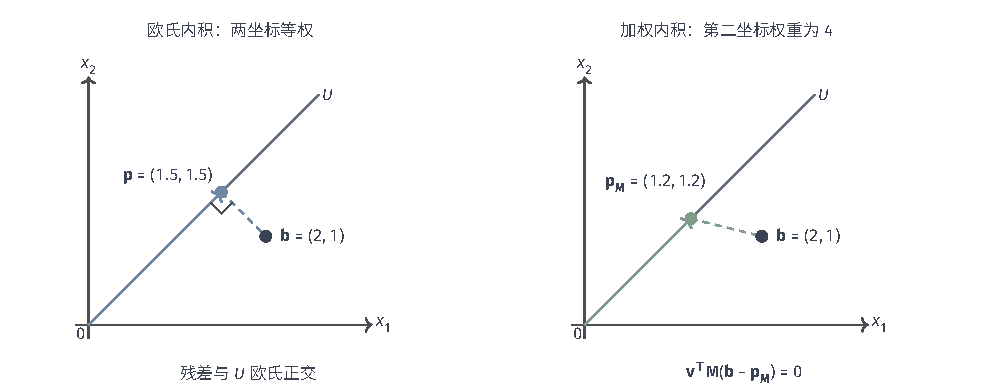
\includegraphics[width=168.998mm]{figures/00-shared/mathematical-preliminaries-upper/02-linear-spaces/tikz/linear-algebra-weighted-projection/figure.pdf}
  \caption{同一目标在同一直线上的欧氏投影与加权投影。实箭头是投影向量，虚线是残差；
  右图画在普通坐标中，残差不必形成欧氏直角。正交性必须用所选内积判断。}
  \label{fig:linear-algebra-weighted-projection}
\end{figure*}



加权问题可以化回普通问题。由定理~\ref{thm:ls-gram-factor}，正定$\bm M$可写成
$\bm M=\bm R^\top\bm R$，$\bm R$可逆。于是
$(\bm A\bm x-\bm b)^\top\bm M(\bm A\bm x-\bm b)=\lVert\bm R\bm A\bm x-\bm R\bm b\rVert_2^2$。
令$\tilde{\bm A}=\bm R\bm A$、$\tilde{\bm b}=\bm R\bm b$，加权目标就是普通平方残差$\lVert\tilde{\bm A}\bm x-\tilde{\bm b}\rVert_2^2$，
加权正规方程~\eqref{eq:linear-algebra-weighted-normal-equations}就是$\tilde{\bm A}^\top\tilde{\bm A}\hat{\bm x}=\tilde{\bm A}^\top\tilde{\bm b}$。
这一步常称\term{白化}（whitening）：先用$\bm R$把各坐标的误差变换到同一欧氏尺度。
于是前面的结论都可以搬过来：加权正规方程总有解；$\bm R$可逆使$\ker\tilde{\bm A}=\ker\bm A$，
所以解唯一的条件仍是$\bm A$满列秩。权重只移动最近点，不改变唯一性。

计算时把$\bm A,\bm b,\bm M$作为输入，先用Cholesky得到权重因子$\bm R$，再形成$\tilde{\bm A},\tilde{\bm b}$。对这对数据运行前面的QR或迭代最小二乘求解器，所得$\hat{\bm x}$就是原变量的解，无需再次变换未知量。输出时核验$\bm A^\top\bm M(\bm b-\bm A\hat{\bm x})$，并报告加权残差长度；普通残差的欧氏正交性已经不是这里的最优性条件。

\subsection{结果检验}
\label{sec:ls-least-squares-verification}

最小二乘的残差一般不为零，所以“残差小”不能作为合格标准；合格标准是残差与列空间正交。
算出$\hat{\bm x}$后分别核验三项。第一，正规方程残差$\bm g=\bm A^\top(\bm b-\bm A\hat{\bm x})$是否在容限内为零，
它检验的正是正交性判据。第二，输出残差$\bm r=\bm b-\bm A\hat{\bm x}$的长度，它是$\bm b$到列空间的距离，
说明模型能解释观测到什么程度。第三，若要求最小范数解，检查$\hat{\bm x}$是否与$\ker\bm A$正交。

用示例~\ref{ex:ls-normal-equations-three-by-two}核对：$\hat{\bm x}=(1,2)^\top$时$\bm r=(1,1,-1)^\top$，$\bm A^\top\bm r=(0,0)^\top$，第一项通过；
$\lVert\bm r\rVert_2=\sqrt3$，这是无法再减小的距离；$\bm A$满列秩，$\ker\bm A=\{\bm0\}$，第三项自动满足。

加权问题按原目标核验：检查加权正规方程~\eqref{eq:linear-algebra-weighted-normal-equations}的残差
$\bm A^\top\bm M(\bm b-\bm A\hat{\bm x})$，并报告$\bm M$加权的残差长度。白化后的残差（用$\bm M=\bm R^\top\bm R$的因子$\bm R$变换后的$\bm R\bm r$）与它长度相同，
但坐标已经变换，不能当作原观测的残差逐项解读。

\section{线性方程与最小二乘方法的比较}

前面的算法都围绕线性关系展开，但返回的对象并不相同。选择方法前，应先确定任务要求满足方程、最小化残差，还是在多个最优解中选出长度最小的一个；随后再检查矩阵结构和可用的数据访问方式。

\subsection{求解目标与方法适用性}

相容方程要求原残差为零。若零空间非平凡，这仍不能唯一决定未知量：从一个解加上任何零空间向量，输出都不变。最小范数要求解与零空间正交，是额外的选解条件。

不相容问题的原残差不能消失。欧氏最小二乘要求正规残差为零；如果又要求最小范数，还须使解位于行空间。因而“残差下降”“达到最小二乘解”和“得到最小范数解”是三种不同的判断，不能用同一个停止量代替。

\subsection{矩阵条件}

表中“矩阵作用”指能够计算矩阵与向量的乘积，不必保存整个矩阵。迭代法的条件指本章已经建立保证的情形；一般矩阵上的表现不能由方法名称保证。

\begin{center}
\small
\begin{tabular}{p{0.24\textwidth}p{0.65\textwidth}}
\toprule
方法 & 适用条件与主要输出\\
\midrule
LU & 可逆方阵；选主元消元后求精确方程的解\\
Cholesky & 对称正定方阵；分解可供多个右端复用\\
块LDL$^\top$ & 对称可逆矩阵，可含不定性；需要对称选主元\\
Schur补 & 已知分块且被消去的块可逆；先求约化方程\\
Woodbury & 已有可复用的基矩阵求解器，更新秩较低\\
Richardson & 对称正定时可按谱范围选步长；只用矩阵作用\\
Jacobi & 对角非零；严格行对角占优保证收敛，正定本身不够\\
Gauss--Seidel & 严格行对角占优或对称正定；逐行原位更新\\
SOR、SSOR & 对称正定且$0<\omega<2$；顺序扫掠或双向扫掠\\
CG & 对称正定；短递推，最小化能量范数误差\\
GMRES & 一般非奇异方阵；最小化原残差，需保存搜索基\\
MINRES & 对称非奇异方阵，可不定；最小化原残差\\
BiCG & 一般非对称方阵；需要矩阵及转置作用，可能失效\\
BiCGSTAB & 一般非对称方阵；无需转置作用，仍须检查失效\\
\bottomrule
\end{tabular}
\end{center}

矩形问题还需要比较求解目标。下面几种方法直接以最小二乘或行投影为出发点，不必先把原矩阵改成方阵。

\begin{center}
\small
\begin{tabular}{p{0.24\textwidth}p{0.65\textwidth}}
\toprule
方法 & 适用条件与主要输出\\
\midrule
正规方程法 & 满列秩最小二乘；形成正规矩阵会平方条件数\\
QR & 满列秩最小二乘；正交变换后求三角方程\\
SVD & 包括秩亏情形；给出秩、最小残差与最小范数代表\\
LSQR、LSMR & 矩形矩阵与转置作用；分别侧重原残差和正规残差\\
Kaczmarz & 相容系统，逐行访问；零初值选出最小范数解\\
扩展Kaczmarz & 允许不相容，需行列访问及辅助向量；概率保证另论\\
\bottomrule
\end{tabular}
\end{center}

左乘可逆矩阵保持精确方程的解集，却一般改变不相容问题中残差的权重。右换元保持可达到的输出，但欧氏最小范数随坐标尺度改变。把问题转换成某算法能够接收的形状以后，还要检查求解目标是否仍是原来的目标。

\subsection{计算开销与收敛速度}

稠密$n$阶LU、Cholesky、QR分解的工作量都为$O(n^3)$，因子的存储为$O(n^2)$；Cholesky利用对称性减少常数。分解完成后，每个新右端通常只需$O(n^2)$的三角求解。对$m\ge d$的稠密矩形矩阵，QR的主要工作量为$O(md^2)$。稀疏情形不能直接把这些估计中的维数换成非零元数，因为消元可能产生填充。

若矩阵有$s$个非零元，一次矩阵作用通常为$O(s)$。CG与BiCGSTAB等短递推保存常数个工作向量；完整GMRES的第$k$步还需对$k$个旧向量正交化，增加$O(kn)$工作和$O(kn)$存储。LSQR与LSMR每步使用一次矩阵作用和一次转置作用，工作向量总长度与$m+d$同阶。重正交化会改变这一存储估计。

因此总成本是每轮代价乘以达到要求所需的轮数，还要加上预条件构造和应用成本。只比较迭代次数，或只比较一次矩阵作用，都不足以判断哪个方法更省。

\subsection{数值稳定性}

正交变换避免了换基中的长度放大，因而QR常比显式形成正规方程更可靠；它仍不能消除原矩阵的小奇异值。SVD揭示这些方向，却也不能从带噪数据中恢复本来就不确定的分量。截断和惩罚会改变问题，应与单纯改善计算过程区别开来。

迭代结束时重新计算原残差。最小二乘还检查正规残差，并结合矩阵尺度解释容差。递推残差很小而真实残差较大，说明舍入误差已影响递推；相邻解几乎不变则可能只是停滞。若数据本身只精确到一定尺度，过度降低计算残差未必改善最终解。

\subsection{典型场景中的取舍}

对中等规模的稠密可逆方阵，可以从带选主元LU开始；若已知对称正定，改用Cholesky。多个右端共用矩阵时，复用分解通常比重复启动迭代更合适。已有分解而矩阵只发生低秩修改时，再检查Woodbury的小系统是否可逆、是否值得复用。

对大型稀疏对称正定系统，可以使用预条件CG；对称不定时考虑保持对称结构的MINRES。一般非对称系统中，GMRES用较多存储换取明确的残差最小化，BiCGSTAB用短递推减少存储，但需接受残差波动及失效检查。

对稠密矩形最小二乘，满列秩时可用QR；需要识别秩或最小范数时使用SVD。大型矩形问题若提供矩阵与转置作用，可用LSQR或LSMR；只方便逐行读取且系统相容时，行投影才直接符合数据访问方式。算法的选择由目标、结构与成本共同决定。


\section{伪逆}
\label{sec:ls-pseudoinverse}

到这里，三种情况各有各的答案。$\bm A$可逆时，唯一解是$\bm A^{-1}\bm b$；满行秩而有无穷多解时，
最小范数解是$\bm A^\top(\bm A\bm A^\top)^{-1}\bm b$；满列秩而无解时，最小二乘解是$(\bm A^\top\bm A)^{-1}\bm A^\top\bm b$。
三个公式各自要求一种满秩，而一般的$\bm A$可能既不满行秩、也不满列秩，这时方程可能无解，
最小二乘解又不唯一，需要先取最近点、再在最近点的全部原像中取范数最小者。
本小节用第~\ref{chap:linear-analysis}章的奇异值分解构造一个矩阵$\bm A^\dagger$，
使$\bm A^\dagger\bm b$在任何秩下都给出这样两次选择的结果，再说明前面三个公式都是它的特例。

\subsection{用SVD构造统一的解}

设$\bm A\in\mathbb R^{m\times d}$的秩为$r$，奇异值分解为~\eqref{eq:matrix-analysis-svd-rank-one-sum}，
$\sigma_1\geq\cdots\geq\sigma_r>0$；按第~\ref{sec:ls-svd}节的构造，把$\bm u_1,\ldots,\bm u_r$与$\bm v_1,\ldots,\bm v_r$
分别扩充为$\mathbb R^m$与$\mathbb R^d$的标准正交基。那里已经说明，$\operatorname{range}(\bm A)$由$\bm u_1,\ldots,\bm u_r$张成，
$\ker\bm A$由$\bm v_{r+1},\ldots,\bm v_d$张成。

$\bm A$把$\bm v_i$伸缩为$\sigma_i\bm u_i$，反向自然应把$\bm u_i$送回$\bm v_i/\sigma_i$。
按两次选择的要求分配$\bm b$的各个分量：把$\bm b$按$\bm u_i$展开，分量$\bm u_i^\top\bm b$（$i\leq r$）配给$\bm v_i/\sigma_i$；
落在$\operatorname{range}(\bm A)^\perp$中的分量（$i>r$）没有原像，直接丢弃，这对应取最近点；
零空间方向$\bm v_{r+1},\ldots,\bm v_d$不分配任何分量，这对应在原像中取范数最小者。

\begin{definition}[Moore--Penrose伪逆]
\label{def:matrix-analysis-pseudoinverse}
设$\bm A$有奇异值分解~\eqref{eq:matrix-analysis-svd-rank-one-sum}。$\bm A$的\term{Moore--Penrose伪逆}（Moore--Penrose pseudoinverse）为
\begin{equation}
 \bm A^\dagger=\sum_{i=1}^r\frac{1}{\sigma_i}\bm v_i\bm u_i^\top,
 \label{eq:matrix-analysis-pseudoinverse}
\end{equation}
$\bm A=\bm0$时规定$\bm A^\dagger=\bm0$。
\end{definition}

用于计算时不必先形成整个伪逆矩阵。输入$\bm A,\bm b$后，计算紧致SVD；对每个非零奇异值依次计算$c_i=\bm u_i^\top\bm b$与$z_i=c_i/\sigma_i$，最后组合$\hat{\bm x}=\sum_{i=1}^r z_i\bm v_i$。输出包含解及原残差；若数据只能确定数值秩，还要报告采用的阈值，因为丢掉正的小奇异值就转为后面的截断求解。

下面在精确秩已知的条件下，证明这样构造的矩阵恰好完成了上面的两次选择。
\begin{theorem}[最小二乘与最小范数]
\label{thm:matrix-analysis-pseudoinverse-minimum-norm}
给定$\bm A\in\mathbb R^{m\times d}$和$\bm b\in\mathbb R^m$，全部最小二乘解为
\begin{equation}
\begin{gathered}
\hat{\bm x}=\bm A^\dagger\bm b+\bm z\\
\bm z\in\ker\bm A,
\end{gathered}
\label{eq:ls-all-pseudoinverse-solutions}
\end{equation}
其中$\bm A^\dagger\bm b$是唯一的最小欧氏范数解；方程相容时，它就是全部精确解中范数最小者。
\end{theorem}
\begin{proof}
把$\bm b$与$\bm x$分别按左、右奇异向量展开，记$b_i=\bm u_i^\top\bm b$、$c_i=\bm v_i^\top\bm x$。由$\bm A\bm x=\sum_{i\leq r}\sigma_ic_i\bm u_i$与$\bm u_1,\ldots,\bm u_m$标准正交，
\[
 \lVert\bm A\bm x-\bm b\rVert_2^2
 =\sum_{i=1}^r(\sigma_ic_i-b_i)^2+\sum_{i=r+1}^m b_i^2 .
\]
第二项与$\bm x$无关；第一项当且仅当$c_i=b_i/\sigma_i$（$i\leq r$）时为零，而$c_{r+1},\ldots,c_d$可以任取。前者正是$\bm A^\dagger\bm b$的坐标，后者组成$\ker\bm A$中的任意向量，所以最小二乘解恰为$\bm A^\dagger\bm b+\bm z$，$\bm z\in\ker\bm A$。由于$\bm A^\dagger\bm b$只含$\bm v_1,\ldots,\bm v_r$方向，它与$\bm z$正交，$\lVert\bm x\rVert_2^2=\lVert\bm A^\dagger\bm b\rVert_2^2+\lVert\bm z\rVert_2^2$，最小值仅在$\bm z=\bm0$时达到。方程相容时第二项为零，最小二乘解就是精确解，论证不变。
\end{proof}

\paragraph{三种情况的统一}

定理对$\bm A$的秩和$\bm b$的位置都没有要求，所以前面分别处理的情况都包含在其中。
方程相容时，最近点就是$\bm b$本身，$\bm A^\dagger\bm b$是精确解中范数最小的一个：解唯一时它就是那个解，
有无穷多解时它就是第~\ref{sec:ls-select-among-solutions}节的最小范数解。方程无解时，$\bm A^\dagger\bm b$是最小二乘解；
最小二乘解唯一时它就是那一个，不唯一时它是其中范数最小者。

三个满秩公式由此成为特例。$\bm A$满列秩时$\ker\bm A=\{\bm0\}$，最小二乘解唯一，
所以对每个$\bm b$都有$\bm A^\dagger\bm b=(\bm A^\top\bm A)^{-1}\bm A^\top\bm b$，即$\bm A^\dagger=(\bm A^\top\bm A)^{-1}\bm A^\top$。
$\bm A$满行秩时每个右端都相容，$\bm A^\dagger\bm b$是最小范数精确解，由第~\ref{sec:ls-select-among-solutions}节，
$\bm A^\dagger=\bm A^\top(\bm A\bm A^\top)^{-1}$。$\bm A$可逆时两种情形同时成立，两个公式都化为$\bm A^{-1}$，所以$\bm A^\dagger=\bm A^{-1}$。
下面用一个欠定方程核对满行秩的情形。

\begin{example}[欠定方程的伪逆]
\label{ex:ls-pinv-underdetermined}
欠定方程$2x_1=3$的系数矩阵$\bm A=[2\ 0]$满行秩，右端$\bm b=(3)$。$\bm A$的奇异值分解只有一项：
$\sigma_1=2$、$\bm u_1=(1)$、$\bm v_1=(1,0)^\top$。和式~\eqref{eq:matrix-analysis-pseudoinverse}给出
\[
 \bm A^\dagger=\frac12\bm v_1\bm u_1^\top=\begin{bmatrix}1/2\\0\end{bmatrix},
\]
与满行秩公式$\bm A^\top(\bm A\bm A^\top)^{-1}=(2,0)^\top/4$一致。$\bm A^\dagger\bm b=(3/2,0)^\top$
正是全部解$(3/2,t)^\top$中范数最小的一个。
\end{example}

秩亏而又不相容时，两次选择都真正起作用，满秩公式一个也用不上。

\begin{example}[秩亏且不相容时的两次选择]
\label{ex:ls-pinv-two-selections}
取$\bm A=\left[\begin{smallmatrix}1&1\\0&0\end{smallmatrix}\right]$、$\bm b=(2,1)^\top$。$\bm A$的秩为$1$，既不满行秩，也不满列秩。
可达输出都形如$(s,0)^\top$，其中离$\bm b$最近的是$(2,0)^\top$，残差$(0,1)^\top$无法消除。
$(2,0)^\top$的原像是直线$x_1+x_2=2$，由示例~\ref{ex:ls-min-norm-line}，其上最靠近原点的点是$(1,1)^\top$。
用和式核对：$\bm A$只有一个正奇异值$\sigma_1=\sqrt2$，对应$\bm u_1=(1,0)^\top$、$\bm v_1=(1,1)^\top/\sqrt2$，于是
\[
\begin{gathered}
\bm A^\dagger=\frac1{\sqrt2}\bm v_1\bm u_1^\top=\frac12\begin{bmatrix}1&0\\1&0\end{bmatrix}\\
\bm A^\dagger\bm b=\begin{bmatrix}1\\1\end{bmatrix}.
\end{gathered}
\]
两次选择的结果与和式一致。
\end{example}

图~\ref{fig:matrix-analysis-pseudoinverse-selections}画出这两次选择。
伪逆既没有让无解的方程变得可解，也没有恢复被$\bm A$消去的信息，它只是在两处都作了最小化选择。

\begin{figure*}[htbp]
  \centering
  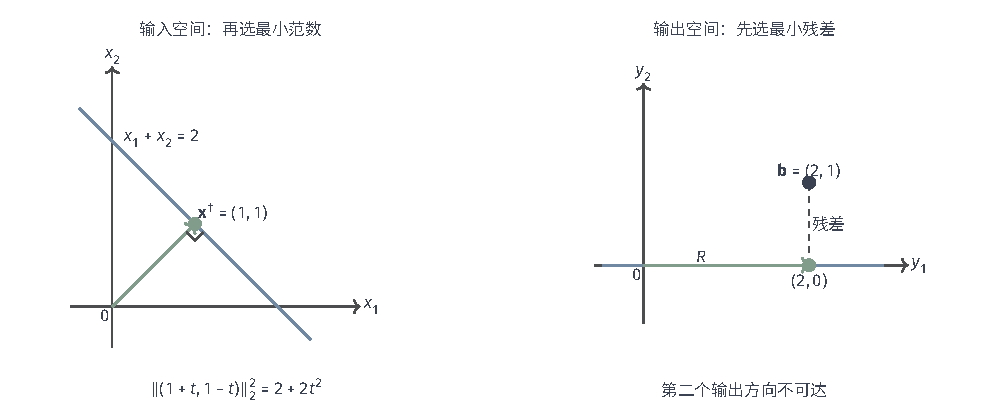
\includegraphics[width=168.998mm]{figures/00-shared/mathematical-preliminaries-upper/02-linear-spaces/tikz/matrix-analysis-pseudoinverse-selections/figure.pdf}
  \caption{伪逆的两次选择。右图先在可达输出中选择离$\bm b=(2,1)^\top$最近的
  $(2,0)^\top$；左图再在整条原像直线$x_1+x_2=2$上选择最靠近原点的$(1,1)^\top$。
  两图属于不同空间，各自等比例绘制。}
  \label{fig:matrix-analysis-pseudoinverse-selections}
\end{figure*}

\subsection{Penrose条件与两个投影}

两次选择也可以用投影矩阵表达。由和式直接相乘，
\[
 \begin{gathered}
\bm A\bm A^\dagger=\sum_{i\leq r}\bm u_i\bm u_i^\top\\
\bm A^\dagger\bm A=\sum_{i\leq r}\bm v_i\bm v_i^\top ,
 \end{gathered}
\]
前者是到$\operatorname{range}(\bm A)$的正交投影，后者是到$(\ker\bm A)^\perp=\operatorname{range}(\bm A^\top)$的正交投影
（式~\eqref{eq:linear-algebra-orthogonal-projector}）。也就是说，$\bm A^\dagger$先把输出正交投影到$\operatorname{range}(\bm A)$，
再在$\operatorname{range}(\bm A^\top)$上反演$\bm A$。

奇异值分解并不唯一，伪逆却不依赖分解的具体选取。由上面两个投影，$\bm A^\dagger$满足四条Penrose条件：
\[
 \begin{gathered}
\bm A\bm A^\dagger\bm A=\bm A\\
\bm A^\dagger\bm A\bm A^\dagger=\bm A^\dagger\\
(\bm A\bm A^\dagger)^\top=\bm A\bm A^\dagger\\
(\bm A^\dagger\bm A)^\top=\bm A^\dagger\bm A .
 \end{gathered}
\]
满足这四条的矩阵只有一个，所以无论用哪个奇异值分解代入和式，得到的都是同一个矩阵。

下面证明唯一性。

设$\bm G$也满足四条条件。由第一条，$(\bm A\bm G)^2=(\bm A\bm G\bm A)\bm G=\bm A\bm G$，即$\bm A\bm G$幂等，
且$\operatorname{range}(\bm A\bm G)=\operatorname{range}(\bm A)$（$\subseteq$显然，$\supseteq$由$\bm A=\bm A\bm G\bm A$）；
同理$\bm G\bm A$幂等，且$\ker(\bm G\bm A)=\ker\bm A$（$\supseteq$显然，$\subseteq$由$\bm A=\bm A\bm G\bm A$）。
后两条说明它们对称，而由第~\ref{sec:ls-projection-matrices}节，对称的幂等矩阵就是到其像的正交投影。
$\bm A\bm G$与$\bm A\bm A^\dagger$都是到$\operatorname{range}(\bm A)$的正交投影，所以$\bm A\bm G=\bm A\bm A^\dagger$。
对称矩阵的像是其零空间的正交补，所以$\bm G\bm A$与$\bm A^\dagger\bm A$都是到$(\ker\bm A)^\perp$的正交投影，$\bm G\bm A=\bm A^\dagger\bm A$。再由第二条，
\[
 \bm G=\bm G\bm A\bm G=(\bm A^\dagger\bm A)\bm G=\bm A^\dagger(\bm A\bm G)=\bm A^\dagger\bm A\bm A^\dagger=\bm A^\dagger .
\]

至此，三种情况的答案统一为$\bm A^\dagger\bm b$。实际计算中，满秩时仍用前面各小节基于分解的方法，
不必为此计算奇异值分解；伪逆的作用在于给出一个对任何秩都成立的统一描述。

不过伪逆有一个与逆矩阵不同的性质：它关于矩阵不连续。非零标量$\varepsilon$的伪逆是$1/\varepsilon$，零的伪逆却是$0$，
$\varepsilon\to0$时前者趋于无穷，而不是趋于后者。原因在于和式中的增益$1/\sigma_i$：小奇异值被放大成大增益。
数据带有误差时，这种放大意味着什么，是下一节要回答的问题。

\section{方程与最小二乘的误差分析}
\label{sec:ls-numerical-sensitivity}

前面各小节都假定$\bm A$与$\bm b$精确，并在精确算术下求解。实际数据带有测量误差，计算又有舍入误差，
所以还要问：输入有一点误差时，算出的解会偏离多少？残差小时，解是否就准确？
第~\ref{chap:linear-analysis}章已经回答了最简单的情形：可逆方程只有右端带误差时，
解的相对误差不超过条件数$\kappa(\bm A)$乘右端的相对误差（定理~\ref{thm:matrix-analysis-condition-number-bound}），
而在欧氏范数下$\kappa_2(\bm A)$是最大与最小奇异值之比。本节从这里出发，先处理系数矩阵也带误差的情形，
再说明真解未知时怎样由残差判断算出的解，然后分析最小二乘的三类输出。分析会显示，误差放大的根源都在小奇异值，
求解方法还可能额外放大误差；最后据此介绍数据与计算两方面的改进。

\subsection{右端项与系数矩阵的有限扰动}
\label{sec:ls-equation-sensitivity}
\label{sec:ls-linear-system-sensitivity}

\paragraph{右端扰动}

先看只改右端的情形。

设$\bm A$可逆，右端由$\bm b$变为$\bm b+\Delta\bm b$，解的变化为$\Delta\bm x=\bm A^{-1}\Delta\bm b$。
由$\lVert\bm A^{-1}\rVert_2=1/\sigma_{\min}(\bm A)$，右端误差落在小奇异值方向时被放大$1/\sigma_{\min}$倍；
换成相对误差，放大倍数不超过$\kappa(\bm A)$。下面用两个$2\times2$例子对照。

\begin{example}[良态方程的右端扰动]
\label{ex:ls-rhs-perturbation-well-conditioned}
取$\bm A_1=\operatorname{diag}(2,1)$，$\kappa_2(\bm A_1)=2$。右端由$(2,1)^\top$改为$(2,1.01)^\top$，解由$(1,1)^\top$变为$(1,1.01)^\top$。
两者的相对变化分别为
\[
 \begin{gathered}
\frac{\lVert\Delta\bm b\rVert_2}{\lVert\bm b\rVert_2}=\frac{0.01}{\sqrt5}\approx0.00447\\
\frac{\lVert\Delta\bm x\rVert_2}{\lVert\bm x\rVert_2}=\frac{0.01}{\sqrt2}\approx0.00707,
 \end{gathered}
\]
放大约$1.58$倍，不超过$\kappa_2(\bm A_1)=2$。
\end{example}

\begin{example}[近平行列的右端扰动]
\label{ex:ls-rhs-perturbation-near-parallel}
取$\bm A_2=\left[\begin{smallmatrix}1&1\\0&\varepsilon\end{smallmatrix}\right]$，$0<\varepsilon\ll1$，两列接近同向。
$\bm A_2^\top\bm A_2=\left[\begin{smallmatrix}1&1\\1&1+\varepsilon^2\end{smallmatrix}\right]$的迹为$2+\varepsilon^2$、行列式为$\varepsilon^2$，
两个特征值约为$2$与$\varepsilon^2/2$，所以$\sigma_{\max}\approx\sqrt2$、$\sigma_{\min}\approx\varepsilon/\sqrt2$，$\kappa_2(\bm A_2)\approx2/\varepsilon$。

取$\varepsilon=10^{-2}$、$\bm b=(2,0)^\top$，解为$(2,0)^\top$。只把$\bm b$的第二分量改为$\eta=10^{-2}$，
由$\varepsilon x_2=\eta$与$x_1+x_2=2$得新解$(1,1)^\top$。两者的相对变化分别为
\[
 \begin{gathered}
\frac{\lVert\Delta\bm b\rVert_2}{\lVert\bm b\rVert_2}=\frac{\eta}{2}=0.005\\
\frac{\lVert\Delta\bm x\rVert_2}{\lVert\bm x\rVert_2}=\frac{\lVert(-1,1)^\top\rVert_2}{\lVert(2,0)^\top\rVert_2}=\frac{\sqrt2}{2}\approx0.707,
 \end{gathered}
\]
放大约$141$倍，与$\kappa_2(\bm A_2)\approx200$同量级。
\end{example}

两个例子都没有舍入误差，差别完全来自问题本身。第二例中解的变化$(-1,1)^\top$几乎正沿着$\bm A_2$的小奇异值方向，
所以被放大得最多。

\paragraph{逆矩阵的扰动}
\label{sec:ls-inverse-sensitivity}
\label{sec:ch06-inverse-stability}

$\bm A$本身也带误差时，扰动后的矩阵甚至可能不再可逆。所以设$\bm B=\bm A+\bm E$，要先回答两件事：
$\bm B$是否可逆，$\bm B^{-1}$离$\bm A^{-1}$多远。答案会给出一个“到奇异边界的余量”。

先看可逆性。若$\lVert\bm A^{-1}\bm E\rVert<1$，则$\bm B$可逆。假设$\bm B\bm x=\bm0$，即$\bm A\bm x=-\bm E\bm x$，左乘$\bm A^{-1}$得$\bm x=-\bm A^{-1}\bm E\bm x$，取范数得$\lVert\bm x\rVert\leq\lVert\bm A^{-1}\bm E\rVert\lVert\bm x\rVert$，这只在$\bm x=\bm0$时可能，所以$\ker\bm B=\{\bm0\}$。

再看逆的变化。由$\bm B^{-1}(\bm A-\bm B)\bm A^{-1}=\bm B^{-1}-\bm A^{-1}$，逆差满足精确恒等式
\begin{equation}
 \bm B^{-1}-\bm A^{-1}
 =-\bm B^{-1}\bm E\,\bm A^{-1}.
 \label{eq:ch06-inverse-finite-perturbation}
\end{equation}
右端含有未知的$\bm B^{-1}$，需要先估计它的大小。

对任意$\bm y$，令$\bm x=\bm B^{-1}\bm y$，由$\bm A\bm x=\bm y-\bm E\bm x$得$\bm x=\bm A^{-1}\bm y-\bm A^{-1}\bm E\bm x$，取范数并移项，$\lVert\bm x\rVert\leq\lVert\bm A^{-1}\rVert\lVert\bm y\rVert/(1-\lVert\bm A^{-1}\bm E\rVert)$，即
\[
 \lVert\bm B^{-1}\rVert\leq\frac{\lVert\bm A^{-1}\rVert}{1-\lVert\bm A^{-1}\bm E\rVert}.
\]
代入恒等式，$\lVert\bm B^{-1}-\bm A^{-1}\rVert\leq\lVert\bm B^{-1}\rVert\lVert\bm E\rVert\lVert\bm A^{-1}\rVert$。两边除以$\lVert\bm A^{-1}\rVert$，并用$\lVert\bm A^{-1}\bm E\rVert\leq\lVert\bm A^{-1}\rVert\lVert\bm E\rVert=\kappa(\bm A)\lVert\bm E\rVert/\lVert\bm A\rVert$。为了用这个较易计算的上界替换分母，还需假设$\kappa(\bm A)\lVert\bm E\rVert/\lVert\bm A\rVert<1$；在此条件下得到
\[
 \frac{\lVert\bm B^{-1}-\bm A^{-1}\rVert}
      {\lVert\bm A^{-1}\rVert}
 \leq
 \frac{\kappa(\bm A)\,\lVert\bm E\rVert/\lVert\bm A\rVert}
      {1-\kappa(\bm A)\,\lVert\bm E\rVert/\lVert\bm A\rVert}.
\]
分子是条件数乘相对扰动，分母是到奇异边界的余量。$\kappa(\bm A)\lVert\bm E\rVert/\lVert\bm A\rVert$接近$1$时界急剧变大；
它不小于$1$时本界失效，但这不等于$\bm B$一定奇异。下面的对角例子说明，这个界可以取等号，余量趋于零时逆矩阵的变化确实无界。

\begin{example}[接近奇异边界的对角矩阵]
\label{ex:ls-inverse-perturbation-diagonal}
取$\bm A=\operatorname{diag}(1,\varepsilon)$，$0<\varepsilon<1$，则$\kappa_2(\bm A)=1/\varepsilon$。
令$\bm E=\operatorname{diag}(0,-\delta)$，$0<\delta<\varepsilon$，即把第二个对角元减少$\delta$。
逆矩阵的该元由$1/\varepsilon$变为$1/(\varepsilon-\delta)$，相对变化为
\[
 \frac{\lVert\bm B^{-1}-\bm A^{-1}\rVert_2}{\lVert\bm A^{-1}\rVert_2}
 =\frac{1/(\varepsilon-\delta)-1/\varepsilon}{1/\varepsilon}
 =\frac{\delta}{\varepsilon-\delta}.
\]
扰动的相对大小为$\lVert\bm E\rVert_2/\lVert\bm A\rVert_2=\delta$，于是$\kappa_2(\bm A)\lVert\bm E\rVert_2/\lVert\bm A\rVert_2=\delta/\varepsilon$，
上界为$(\delta/\varepsilon)/(1-\delta/\varepsilon)=\delta/(\varepsilon-\delta)$，与实际变化恰好相等。
$\delta\to\varepsilon$时相对变化无界：扰动的相对大小接近$1/\kappa_2(\bm A)=\varepsilon$时，矩阵到达奇异边界。
\end{example}

\paragraph{矩阵与右端同时扰动}

有了逆矩阵的估计，就可以处理一般情形。

设$\bm A$可逆且$\bm b\ne\bm0$，原解$\bm x$因而非零。扰动后的方程为$(\bm A+\bm E)(\bm x+\Delta\bm x)=\bm b+\Delta\bm b$，减去$\bm A\bm x=\bm b$，得$\bm A\Delta\bm x=\Delta\bm b-\bm E\bm x-\bm E\Delta\bm x$。左乘$\bm A^{-1}$并取范数，
\[
 \lVert\Delta\bm x\rVert\leq\lVert\bm A^{-1}\rVert\bigl(\lVert\Delta\bm b\rVert+\lVert\bm E\rVert\lVert\bm x\rVert+\lVert\bm E\rVert\lVert\Delta\bm x\rVert\bigr).
\]
把含$\lVert\Delta\bm x\rVert$的项移到左边，两边除以$\lVert\bm x\rVert$，并用$\lVert\Delta\bm b\rVert/\lVert\bm x\rVert\leq\lVert\bm A\rVert\lVert\Delta\bm b\rVert/\lVert\bm b\rVert$，在$\kappa(\bm A)\lVert\bm E\rVert/\lVert\bm A\rVert<1$时得到
\begin{equation}
 \frac{\lVert\Delta\bm x\rVert}{\lVert\bm x\rVert}
 \leq
 \frac{\kappa(\bm A)}{1-\kappa(\bm A)\lVert\bm E\rVert/\lVert\bm A\rVert}
 \left(
 \frac{\lVert\Delta\bm b\rVert}{\lVert\bm b\rVert}
 +\frac{\lVert\bm E\rVert}{\lVert\bm A\rVert}
 \right).
 \label{eq:matrix-analysis-linear-system-perturbation}
\end{equation}
读法是：两类相对扰动先相加，再被条件数放大，最后除以到奇异边界的余量。
$\bm E=\bm0$时它退回定理~\ref{thm:matrix-analysis-condition-number-bound}的右端扰动界。
这仍是最坏方向上的上界；扰动是否落在放大方向，决定实际误差离这个上界有多远。

\subsection{残差、前向误差与后向误差}
\label{sec:ls-numerical-stability}
\label{sec:ls-data-computation-error}
\label{sec:linear-algebra-error-propagation}
\label{sec:ch06-error-propagation}
\label{sec:ls-result-verification}
\label{sec:matrix-analysis-error-verification}

上面的界比较的是两个精确解。实际手里只有一个算出的候选解$\widehat{\bm x}$，真解未知，怎样判断它的误差？以下仍设$\bm A$可逆且$\bm b\ne\bm0$。
第~\ref{sec:ls-linear-equation-verification}节用残差核验候选解，并提醒残差小不等于解准确；现在可以定量说明这一点。能直接计算的是残差
\begin{equation}
 \bm r=\bm b-\bm A\widehat{\bm x}.
 \label{eq:matrix-analysis-residual}
\end{equation}
由$\bm A(\bm x-\widehat{\bm x})=\bm r$，候选解的误差是$\bm A^{-1}\bm r$，与只改右端的情形相同，相对误差满足
\[
 \frac{\lVert\widehat{\bm x}-\bm x\rVert}{\lVert\bm x\rVert}
 \leq\kappa(\bm A)\frac{\lVert\bm r\rVert}{\lVert\bm b\rVert}.
\]
所以病态时小残差不保证解准确，下面的例子把这一点推到极端。

\begin{example}[反例：残差小而解误差大]
\label{ex:ls-small-residual-large-error}
取$\bm A=\operatorname{diag}(1,\varepsilon)$、$\bm b=(1,\varepsilon)^\top$，$0<\varepsilon\ll1$，精确解为$\bm x=(1,1)^\top$。
候选解$\widehat{\bm x}=(1,0)^\top$的残差为$\bm r=(0,\varepsilon)^\top$，相对残差为$\varepsilon/\sqrt{1+\varepsilon^2}$，随$\varepsilon\to0$趋于零；
相对解误差却是$\lVert(0,-1)^\top\rVert_2/\lVert(1,1)^\top\rVert_2=1/\sqrt2$，不随$\varepsilon$减小。
这与上面的界一致：$\kappa_2(\bm A)=1/\varepsilon$恰好抵消了相对残差中的因子$\varepsilon$。
\end{example}

残差还有另一种读法：把$\widehat{\bm x}$看作某个邻近问题的精确解，问这个邻近问题离原问题多近。
满足$(\bm A+\Delta\bm A)\widehat{\bm x}=\bm b+\Delta\bm b$的最小相对扰动称为\term{后向误差}（backward error）；
与之相对，直接比较答案的误差$\widehat{\bm x}-\bm x$称为\term{前向误差}（forward error）。
允许矩阵与右端同时改变、以相对大小$\max\{\lVert\Delta\bm A\rVert_2/\lVert\bm A\rVert_2,\lVert\Delta\bm b\rVert_2/\lVert\bm b\rVert_2\}$度量时，后向误差为
\begin{equation}
 \eta_2(\widehat{\bm x})
 =\frac{\lVert\bm r\rVert_2}
       {\lVert\bm A\rVert_2\lVert\widehat{\bm x}\rVert_2+\lVert\bm b\rVert_2}.
 \label{def:matrix-analysis-normwise-backward-error}
\end{equation}
先说明它不能更小：若$(\bm A+\Delta\bm A)\widehat{\bm x}=\bm b+\Delta\bm b$且两项相对大小都不超过$\epsilon$，则$\bm r=\Delta\bm A\widehat{\bm x}-\Delta\bm b$，
$\lVert\bm r\rVert_2\leq\epsilon(\lVert\bm A\rVert_2\lVert\widehat{\bm x}\rVert_2+\lVert\bm b\rVert_2)$，即$\epsilon\geq\eta_2$。
再说明它能达到。若$\widehat{\bm x}=\bm0$，取$\Delta\bm A=\bm0$、$\Delta\bm b=-\bm b$即可达到$\eta_2=1$。

若$\widehat{\bm x}\ne\bm0$，记分母为$d_0$，取
\[
 \begin{gathered}
\Delta\bm A=\frac{\lVert\bm A\rVert_2}{d_0\lVert\widehat{\bm x}\rVert_2}\,\bm r\widehat{\bm x}^\top\\
\Delta\bm b=-\frac{\lVert\bm b\rVert_2}{d_0}\,\bm r ,
 \end{gathered}
\]
则$(\bm A+\Delta\bm A)\widehat{\bm x}=\bm b-\bm r+\tfrac{\lVert\bm A\rVert_2\lVert\widehat{\bm x}\rVert_2}{d_0}\bm r=\bm b+\Delta\bm b$，两项的相对大小都等于$\eta_2$。

把后向误差当作式~\eqref{eq:matrix-analysis-linear-system-perturbation}中的数据扰动，就得到常用的经验规则：
前向误差大约不超过条件数乘后向误差。

后向误差的用处在于把算法的质量与问题的病态分开。计算机中的实数运算都有舍入，每次基本运算满足
\begin{equation}
\begin{gathered}
\operatorname{fl}(x\circ y)=(x\circ y)(1+\delta)\\
|\delta|\leq u,
\end{gathered}
\label{eq:ch06-floating-point-model}
\end{equation}
其中$\circ$是加减乘除之一，$u$称为单位舍入，双精度时$u=2^{-53}\approx1.1\times10^{-16}$。这个模型假设运算有定义且结果没有发生溢出或影响相对误差界的下溢。好的算法应当让这些舍入合起来只相当于一个很小的输入扰动。

\begin{definition}[后向稳定]
\label{def:matrix-analysis-backward-stability}
若算法对所有合法输入给出的结果都是某个邻近输入的精确解，且后向误差以$u$乘一个与数据无关的温和常数为界，则称算法\term{后向稳定}（backward stable）。
\end{definition}
正定矩阵的Cholesky分解与Householder QR（第~\ref{sec:ls-orthogonalization-qr}节）具有后向稳定性。带部分主元的LU分解，其后向误差界还依赖消元中的元素增长；增长温和时通常稳定，但不能对所有矩阵保证这个因子都很小。

示例~\ref{ex:ls-partial-pivoting}中不选主元的消元可能产生很大的乘子，把舍入误差放大成很大的输入扰动。

后向稳定只保证$\widehat{\bm x}$是邻近问题的精确解；病态问题中，很小的后向误差经条件数放大，仍可能得到很大的前向误差。
稳定算法不能治愈问题本身的病态，所以报告结果时要同时给出残差或后向误差，以及条件数的估计。

\subsection{最小二乘的不同输出与正规方程的风险}
\label{sec:ls-ls-regularization-sensitivity}
\label{sec:ls-ordinary-ls-sensitivity}

最小二乘有三类输出：系数$\hat{\bm x}=\bm A^\dagger\bm b$、拟合值$\bm A\hat{\bm x}=\bm P_{\operatorname{range}\bm A}\bm b$与残差$\bm b-\bm A\hat{\bm x}$。
它们对扰动的反应不同。

设$\bm A$固定、右端改变$\Delta\bm b$。拟合值的增量是$\bm P_{\operatorname{range}\bm A}\Delta\bm b$，正交投影不放大长度；
残差增量是$(\bm I-\bm P_{\operatorname{range}\bm A})\Delta\bm b$，同样不被放大；系数的增量却是$\bm A^\dagger\Delta\bm b$，
由伪逆的和式，$\lVert\Delta\hat{\bm x}\rVert_2\leq\lVert\Delta\bm b\rVert_2/\sigma_r$，其中$\sigma_r$是最小正奇异值；若$\bm A=\bm0$，伪逆为零，系数的增量也为零。
所以“拟合得好”与“系数可靠”是两回事，不能用一个误差数概括。

\paragraph{近共线设计}

示例~\ref{ex:ls-nearly-collinear-design}显示，拟合可以很好而系数很大。下面用奇异值说明原因。

\begin{example}[近共线设计的奇异值]
\label{ex:ls-nearly-collinear-singular-values}
示例~\ref{ex:ls-nearly-collinear-design}中设计矩阵$\bm X_\varepsilon$的两列是$\bm c_1$与$\bm c_1+\varepsilon\bm q$，
其中$\bm c_1=(1,1,1)^\top$、$\bm q=(0,1,-1)^\top$互相正交，所以两列都位于$\operatorname{span}\{\bm c_1,\bm q\}$内。
以$\bm c_1/\sqrt3$、$\bm q/\sqrt2$为这个平面的正交坐标，两列的坐标分别是$(\sqrt3,0)^\top$与$(\sqrt3,\sqrt2\,\varepsilon)^\top$；
再把全部输出统一除以$\sqrt3$，设计矩阵化为
\begin{equation}
\begin{gathered}
\bm X_{\widetilde\varepsilon}
 =\begin{bmatrix}1&1\\0&\widetilde\varepsilon\end{bmatrix}\\
\widetilde\varepsilon=\sqrt{2/3}\,\varepsilon .
\end{gathered}
\label{eq:matrix-analysis-nearly-collinear-design}
\end{equation}
换成正交坐标不改变奇异值，统一缩放只把奇异值同除以$\sqrt3$，不改变它们的比，所以条件数可以在$\bm X_{\widetilde\varepsilon}$上计算。

Gram矩阵$\bm X_{\widetilde\varepsilon}^\top\bm X_{\widetilde\varepsilon}=\left[\begin{smallmatrix}1&1\\1&1+\widetilde\varepsilon^2\end{smallmatrix}\right]$的迹为$2+\widetilde\varepsilon^2$，
行列式为$\widetilde\varepsilon^2$，特征值为
\begin{equation}
 \lambda_\pm
 =\frac{2+\widetilde\varepsilon^2
          \mathbin{\pm}\sqrt{4+\widetilde\varepsilon^4}}{2}.
 \label{eq:matrix-analysis-nearly-collinear-gram-eigenvalues}
\end{equation}
$\widetilde\varepsilon\to0$时$\lambda_+\to2$，$\lambda_-=\widetilde\varepsilon^2/\lambda_+\approx\widetilde\varepsilon^2/2$，
所以$\bm X_{\widetilde\varepsilon}$的奇异值$\sigma_{\max}\to\sqrt2$、$\sigma_{\min}\approx\widetilde\varepsilon/\sqrt2$，
条件数约为$2/\widetilde\varepsilon=\sqrt6/\varepsilon$。乘回$\sqrt3$，$\bm X_\varepsilon$本身的最小奇异值约为$\sqrt3\,\widetilde\varepsilon/\sqrt2=\varepsilon$。
\end{example}

大奇异值对应的方向近似为两个系数同增同减，小奇异值对应的方向近似为两个系数此增彼减。
响应在后一方向上的分量被放大约$1/\varepsilon$倍，这正是$\hat{\bm w}_\varepsilon$中$\delta/\varepsilon$项的来源。

化简后的$\bm X_{\widetilde\varepsilon}$与示例~\ref{ex:ls-rhs-perturbation-near-parallel}的近平行矩阵$\bm A_2$形状相同，
所以可以在$\bm A_2$上直接看到系数怎样分裂。

\begin{example}[近平行列的系数分裂]
\label{ex:ls-coefficient-splitting}
沿用示例~\ref{ex:ls-rhs-perturbation-near-parallel}的$\bm A_2=\left[\begin{smallmatrix}1&1\\0&\varepsilon\end{smallmatrix}\right]$，
把右端扰动写成一般的$\eta$。右端为$(2,0)^\top$时解为$(2,0)^\top$；右端变为$(2,\eta)^\top$时，由$\varepsilon x_2=\eta$与$x_1+x_2=2$得
\begin{equation}
\begin{gathered}
\hat{\bm x}=\begin{bmatrix}2-\eta/\varepsilon\\ \eta/\varepsilon\end{bmatrix}\\
\Delta\hat{\bm x}=\begin{bmatrix}-\eta/\varepsilon\\ \eta/\varepsilon\end{bmatrix}.
\end{gathered}
\label{eq:matrix-analysis-collinear-coefficient-perturbation}
\end{equation}
系数误差的长度$\sqrt2\,|\eta|/\varepsilon$是右端误差$|\eta|$的$\sqrt2/\varepsilon$倍，两个系数沿相反方向分开。
$\bm A_2$可逆，拟合值始终等于右端本身。
\end{example}

图~\ref{fig:matrix-analysis-coefficient-sensitivity}画出$\varepsilon$减小时两个系数怎样分开。

\begin{figure}
 \centering
 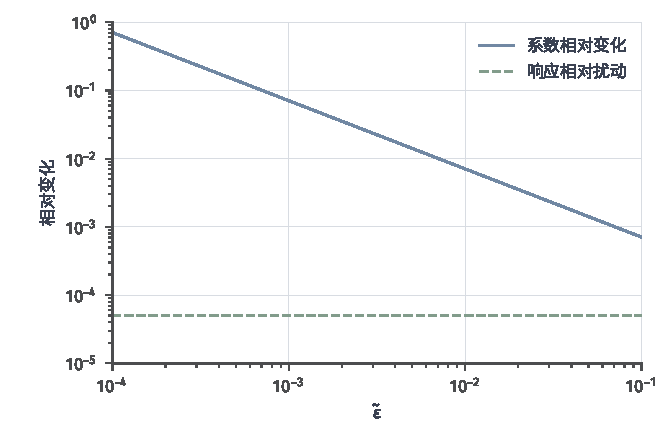
\includegraphics[width=0.92\linewidth]{figures/00-shared/mathematical-preliminaries-upper/02-linear-spaces/matplotlib/matrix-analysis-coefficient-sensitivity/figure.pdf}
 \caption{近平行列的系数分裂：对$\bm A_2=\left[\begin{smallmatrix}1&1\\0&\varepsilon\end{smallmatrix}\right]$固定右端扰动$\eta$，$\varepsilon$越小，两个系数
 沿相反方向偏离$(2,0)$越远，绝对误差随$1/\varepsilon$增长。}
 \label{fig:matrix-analysis-coefficient-sensitivity}
\end{figure}

\paragraph{正规方程的条件数平方}

问题本身的敏感度之外，求解方法也会影响结果。由奇异值分解，$\bm A^\top\bm A$的特征值是$\sigma_i^2$，故满列秩时
\begin{equation}
 \kappa_2(\bm A^\top\bm A)=\kappa_2(\bm A)^2.
 \label{eq:matrix-analysis-normal-equation-condition-square}
\end{equation}
平方的后果在近平行矩阵上看得最清楚。

\begin{example}[形成Gram矩阵时丢失的信息]
\label{ex:ls-gram-rounding-loss}
对示例~\ref{ex:ls-rhs-perturbation-near-parallel}的$\bm A_2$，$\kappa_2(\bm A_2)\approx2/\varepsilon$。
Gram矩阵$\bm A_2^\top\bm A_2=\left[\begin{smallmatrix}1&1\\1&1+\varepsilon^2\end{smallmatrix}\right]$的小特征值约为$\varepsilon^2/2$，条件数约为$4/\varepsilon^2$。
取$\varepsilon=10^{-8}$，则$\varepsilon^2=10^{-16}$已低于双精度的单位舍入$u\approx1.1\times10^{-16}$，
$1+\varepsilon^2$在舍入后就是$1$，存储下来的Gram矩阵成为奇异的$\left[\begin{smallmatrix}1&1\\1&1\end{smallmatrix}\right]$。
而$\bm A_2$本身的条件数约为$2\times10^8$，远未达到$1/u$，它的两列在双精度下仍可区分。
\end{example}

所以形成$\bm A^\top\bm A$这一步就可能把小奇异方向的信息丢掉。这就是第~\ref{sec:ls-qr-method}节的QR方法不形成$\bm A^\top\bm A$的原因：
用Householder反射实现时（第~\ref{sec:ls-orthogonalization-qr}节），它只经过正交变换，不会在问题本身的敏感度之外再把条件数平方。

\subsection{伪逆、秩变化与数值秩}

以上只改右端。矩阵本身改变时，秩是否保持起决定作用。设$\bm A$与$\bm B=\bm A+\bm E$的正奇异值都不小于$s_0>0$。
直接展开右端可验证恒等式
\[
 \bm B^\dagger-\bm A^\dagger
 =-\bm B^\dagger\bm E\bm A^\dagger
 +\bm B^\dagger(\bm I-\bm A\bm A^\dagger)
 -(\bm I-\bm B^\dagger\bm B)\bm A^\dagger .
\]
三项分别估计。非零矩阵满足$\lVert\bm A^\dagger\rVert_2=1/\sigma_r(\bm A)\leq1/s_0$；零矩阵的伪逆也是零，仍满足这个上界。对$\bm B$同理。
第一项不超过$\lVert\bm B^\dagger\rVert_2\lVert\bm E\rVert_2\lVert\bm A^\dagger\rVert_2\leq\lVert\bm E\rVert_2/s_0^2$。
第二项利用Penrose条件写$\bm B^\dagger=\bm B^\dagger(\bm B\bm B^\dagger)^\top=\bm B^\dagger(\bm B^\dagger)^\top\bm B^\top$；
又因$\bm A^\top(\bm I-\bm A\bm A^\dagger)=\bm0$，有$\bm B^\top(\bm I-\bm A\bm A^\dagger)=\bm E^\top(\bm I-\bm A\bm A^\dagger)$，
所以该项不超过$\lVert\bm B^\dagger\rVert_2^2\lVert\bm E\rVert_2\leq\lVert\bm E\rVert_2/s_0^2$。第三项同理。合起来，
\begin{equation}
 \lVert\bm B^\dagger-\bm A^\dagger\rVert_2
 \leq\frac{3\lVert\bm E\rVert_2}{s_0^2}.
 \label{eq:ch06-pseudoinverse-fixed-rank-perturbation}
\end{equation}
这个估计本身不要求两矩阵同秩，关键是它们的正奇异值有共同的正下界。若一列矩阵趋于$\bm A$而秩在极限处下降，就会有正奇异值趋于零，此时不能使用与扰动无关的$s_0$。相反，在固定秩且正奇异值远离零的邻域内，上界直接给出伪逆的连续性。

\begin{example}[反例：秩改变时伪逆不连续]
\label{ex:ls-pinv-discontinuity}
取$\bm A=\operatorname{diag}(1,0)$与$\bm B_\varepsilon=\operatorname{diag}(1,\varepsilon)$，$0<\varepsilon<1$。
二者之差$\lVert\bm B_\varepsilon-\bm A\rVert_2=\varepsilon\to0$，但
\[
 \begin{gathered}
\bm B_\varepsilon^\dagger=\operatorname{diag}(1,1/\varepsilon)\\
\bm A^\dagger=\operatorname{diag}(1,0),
 \end{gathered}
\]
所以$\lVert\bm B_\varepsilon^\dagger-\bm A^\dagger\rVert_2=1/\varepsilon\to\infty$。
$\bm B_\varepsilon$的秩为$2$，$\bm A$的秩为$1$；两者正奇异值的公共下界只能取$s_0=\varepsilon$，
界~\eqref{eq:ch06-pseudoinverse-fixed-rank-perturbation}给出$3\varepsilon/\varepsilon^2=3/\varepsilon$，同样随$\varepsilon\to0$无界。
\end{example}

这将伪逆一节末尾的标量现象扩展到了矩阵，也说明秩变化时新出现的小奇异值为何危险。

实际数据的秩因而要谨慎对待。第~\ref{chap:linear-analysis}章的奇异值扰动界~\eqref{eq:matrix-analysis-singular-value-perturbation}说明，矩阵改变$\bm E$时每个奇异值的移动不超过$\lVert\bm E\rVert_2$，所以小于数据误差尺度的奇异值与零无法区分：它可能是一个真实但很弱的方向，也可能只是噪声。据此，把大于某个阈值$\tau$的奇异值个数称为\term{数值秩}（numerical rank），$\tau$按数据误差的尺度选取。

综合本小节的分析：无论是方程的解、最小二乘的系数还是伪逆本身，误差放大都来自小奇异值。
它们一方面使增益$1/\sigma_i$很大，另一方面在误差尺度下难以与零区分；形成正规方程之类的计算步骤还会进一步损失精度。
前面的QR等方法避免额外引入不稳定计算；下一节转向正则化，通过改变目标来限制数据误差的放大。

\section{正则化与截断求解}
\label{sec:ls-truncated-svd-ridge}

小奇异值会把右端误差放大到解中。提高计算精度只能减少计算误差，不能消除数据本身的不确定性。本节通过限制小奇异值方向上的响应来换取稳定，同时明确所求的问题已发生改变。

\subsection{岭回归与Tikhonov正则化}
\label{sec:ls-regularized-ls}

示例~\ref{ex:ls-nearly-collinear-design}中，系数为了拟合上的微小改进而取得很大。若任务希望输入不要太大，
可以在数据项之外加上输入长度的平方惩罚，得到\term{岭回归}（ridge regression）
\begin{equation}
\begin{gathered}
\min_{\bm x}\ \lVert\bm A\bm x-\bm b\rVert_2^2+\lambda\lVert\bm x\rVert_2^2\\
\lambda>0.
\end{gathered}
\label{eq:ls-ridge-objective}
\end{equation}
参数$\lambda$权衡两项：$\lambda$越大，越倾向于小的输入，拟合误差不会减小；在某些退化情形下它也可能保持不变。

更一般地，惩罚可以作用在希望压小的量$\bm L\bm x$上，$\bm L\in\mathbb R^{p\times d}$，例如相邻分量之差，
得到\term{Tikhonov正则化}（Tikhonov regularization）\scite{math-hansen2008regtools}
\begin{equation}
\begin{gathered}
\min_{\bm x}\ \lVert\bm A\bm x-\bm b\rVert_2^2+\lambda\lVert\bm L\bm x\rVert_2^2\\
\lambda>0.
\end{gathered}
\label{eq:linear-algebra-general-tikhonov}
\end{equation}
两项都是平方长度，而$\lambda\lVert\bm L\bm x\rVert_2^2=\lVert\sqrt\lambda\,\bm L\bm x-\bm0\rVert_2^2$，
所以可以把两个残差向量上下堆成一个更长的残差向量，写成堆叠矩阵的普通最小二乘，
称为\term{增广最小二乘}（augmented least squares）：
\begin{equation}
 \begin{bmatrix}\bm A\\ \sqrt{\lambda}\,\bm L\end{bmatrix}\bm x
 \approx\begin{bmatrix}\bm b\\ \bm0\end{bmatrix}.
 \label{eq:ls-augmented-system}
\end{equation}
对堆叠矩阵套用正规方程~\eqref{eq:linear-algebra-normal-equations}：堆叠矩阵的转置乘自身是
$\bm A^\top\bm A+\lambda\bm L^\top\bm L$，转置乘堆叠右端是$\bm A^\top\bm b$，于是
\begin{equation}
 (\bm A^\top\bm A+\lambda\bm L^\top\bm L)\hat{\bm x}=\bm A^\top\bm b.
 \label{eq:ls-tikhonov-normal}
\end{equation}
它是普通最小二乘，存在性自动成立。由~\eqref{eq:ls-normal-kernel}，系数矩阵的零空间就是堆叠矩阵的零空间，
即同时满足$\bm A\bm x=\bm0$与$\bm L\bm x=\bm0$的向量，所以解唯一当且仅当
\begin{equation}
 \ker\bm A\cap\ker\bm L=\{\bm0\}.
 \label{eq:linear-algebra-tikhonov-common-nullspace}
\end{equation}
$\bm L=\bm I$时条件自动成立，岭回归对任意$\bm A$都有唯一解。其他惩罚则未必。

\begin{example}[反例：惩罚无法确定的方向]
\label{ex:ls-tikhonov-common-nullspace}
取$\bm A=\bm L=[\,1\ -1\,]$。两者的零空间都是$\operatorname{span}\{(1,1)^\top\}$，条件~\eqref{eq:linear-algebra-tikhonov-common-nullspace}不成立。
对任何解$\hat{\bm x}$和任何$t\in\mathbb R$，$\hat{\bm x}+t(1,1)^\top$的数据项与惩罚项都不变，因而也是解。
所以无论$\lambda$多大，都不能确定两个分量的共同水平。
\end{example}

权重与惩罚也可以同时使用，目标
$(\bm A\bm x-\bm b)^\top\bm M(\bm A\bm x-\bm b)+\lambda\lVert\bm L\bm x\rVert_2^2$的正规方程为
\begin{equation}
 (\bm A^\top\bm M\bm A+\lambda\bm L^\top\bm L)\hat{\bm x}=\bm A^\top\bm M\bm b,
 \label{eq:ls-general-normal-equations}
\end{equation}
$\bm M$正定、$\lambda>0$时，解唯一的条件仍是~\eqref{eq:linear-algebra-tikhonov-common-nullspace}。
要注意，加惩罚改变的是问题本身：选择$\lambda$是在重新设定任务，而不是让原方程“算得出来”的数值技巧。

$\lambda$怎样影响解，可以在奇异值坐标中读出。岭回归的正规方程是$(\bm A^\top\bm A+\lambda\bm I)\bm x=\bm A^\top\bm b$。在右奇异向量坐标$c_i=\bm v_i^\top\bm x$中，
$\bm A^\top\bm A$与$\bm I$同时成为对角矩阵，方程按方向分开：$i\leq r$时$(\sigma_i^2+\lambda)c_i=\sigma_i\,\bm u_i^\top\bm b$，
$i>r$时$\lambda c_i=0$，故$c_i=0$。于是
\begin{equation}
\begin{gathered}
\hat{\bm x}_\lambda=\sum_{i=1}^r\frac{\sigma_i}{\sigma_i^2+\lambda}\,(\bm u_i^\top\bm b)\,\bm v_i
 =\sum_{i=1}^r f_i\,\frac{\bm u_i^\top\bm b}{\sigma_i}\,\bm v_i\\
f_i=\frac{\sigma_i^2}{\sigma_i^2+\lambda}.
\end{gathered}
\label{eq:matrix-analysis-ridge-filter-factor}
\end{equation}
前一种写法说明，岭回归把伪逆中的增益$1/\sigma_i$换成了$\sigma_i/(\sigma_i^2+\lambda)$。由$\sigma_i^2+\lambda\geq2\sigma_i\sqrt\lambda$，
新的增益不超过$1/(2\sqrt\lambda)$，不再随$\sigma_i\to0$而爆炸。

后一种写法把它与最小范数解比较：每个方向多乘了一个介于$0$与$1$之间的\term{滤波因子}（filter factor）$f_i$。
$\sigma_i^2\gg\lambda$时$f_i\approx1$，该方向几乎不受影响；$\sigma_i^2\ll\lambda$时$f_i\approx\sigma_i^2/\lambda$，该方向被压低，增益约为$\sigma_i/\lambda$；
$\sigma_i^2=\lambda$处$f_i$恰为$1/2$。代价是大奇异值方向也被轻微压缩，$f_i$总小于$1$。下面在近共线设计上看两个$\lambda$的效果。

\begin{example}[近共线设计上的岭回归]
\label{ex:ls-ridge-nearly-collinear}
沿用示例~\ref{ex:ls-nearly-collinear-design}的$\bm X_\varepsilon$与$\bm y$，取$\varepsilon=0.01$、$\delta=0.1$。
直接计算可得两个奇异值约为$\sigma_1\approx2.449$、$\sigma_2\approx0.0100$，
对应的右奇异向量近似为$(1,1)^\top/\sqrt2$与$(1,-1)^\top/\sqrt2$。精确最小二乘解是$(-9,10)^\top$，残差为零；
它的大系数全部来自第二个方向，该方向的系数$\bm u_2^\top\bm y/\sigma_2$的绝对值约为$0.134/0.0100\approx13.4$。
按式~\eqref{eq:matrix-analysis-ridge-filter-factor}计算两个$\lambda$下的结果：
\[
 \begin{array}{cccc}
  \lambda & f_2 & \hat{\bm x}_\lambda & \lVert\bm X_\varepsilon\hat{\bm x}_\lambda-\bm y\rVert_2\\[2pt]
  10^{-4} & \approx0.50 & \approx(-4.25,\,5.25)^\top & \approx0.067\\
  10^{-2} & \approx0.0099 & \approx(0.41,\,0.59)^\top & \approx0.133
 \end{array}
\]
$\lambda=10^{-4}\approx\sigma_2^2$时，第二个方向保留一半；$\lambda=10^{-2}$时，第二个方向几乎被去掉。
第一个方向的因子$f_1$在两种情形下都大于$0.998$。所以随着$\lambda$增大，解从精确拟合的大系数逐渐移向两个系数平分共同作用的解，
代价是残差增大。
\end{example}

计算岭回归不必作奇异值分解，上面的滤波因子只用于解释$\lambda$的作用。正规方程$(\bm A^\top\bm A+\lambda\bm I)\hat{\bm x}=\bm A^\top\bm b$的系数矩阵对任意$\bm A$都正定，
可以用Cholesky分解；更可靠的做法是对堆叠矩阵~\eqref{eq:ls-augmented-system}作QR分解，避免形成$\bm A^\top\bm A$。
一般的Tikhonov惩罚（$\bm L\neq\bm I$）不能由$\bm A$一个矩阵的奇异值分解按方向分开，但同样可以用堆叠矩阵的QR分解求解。

这给出统一的计算步骤：输入$\bm A,\bm b,\bm L$与选定的$\lambda>0$，组成增广系数$\bm F=[\bm A^\top\;\sqrt\lambda\bm L^\top]^\top$和增广右端$\bm c=(\bm b^\top,\bm0^\top)^\top$。若公共零空间为零，对$\bm F$作经济型QR分解$\bm F=\bm Q_F\bm R_F$，计算$\bm g=\bm Q_F^\top\bm c$，回代$\bm R_F\hat{\bm x}_\lambda=\bm g$。公共零空间非零时，改用SVD并声明选择最小范数解。整个过程输出的是正则化目标的解，不能再用原来无惩罚的正规残差为零作为验收条件。

核验时要回到原目标，分别报告数据项$\lVert\bm A\hat{\bm x}-\bm b\rVert_2^2$（加权时为$\bm M$加权长度）、惩罚项$\lambda\lVert\bm L\hat{\bm x}\rVert_2^2$
以及正规方程~\eqref{eq:ls-general-normal-equations}的残差，不能只报告堆叠问题的残差。

\subsection{截断SVD求解}

这里的输入除$\bm A,\bm b$外，还包括保留阶数$k$或奇异值阈值$\tau$。

先将奇异值按降序排列，再保留前$k$个方向；若用阈值，则令$k$等于满足$\sigma_i>\tau$的个数。对保留方向计算$c_i=\bm u_i^\top\bm b$、$z_i=c_i/\sigma_i$，再组合输出。没有方向被保留时输出零向量。

这里$k$表示保留阶数，不是迭代次数；后面的$\bm x_k$是这一阶数对应的截断解。

岭回归按滤波因子连续地压低小奇异值方向。更直接的做法是只在前$k$个奇异方向上反演，丢弃其余方向：
\[
\begin{gathered}
\bm x_k=\sum_{i=1}^k\frac{\bm u_i^\top\bm b}{\sigma_i}\,\bm v_i\\
1\leq k\leq r ,
\end{gathered}
\]
相当于滤波因子只取$1$（$i\leq k$）或$0$（$i>k$）。$k=r$时它就是$\bm A^\dagger\bm b$；$k<r$时，它恰是把$\bm A$换成第~\ref{sec:ls-svd}节的截断SVD$\bm A_k=\sum_{i\leq k}\sigma_i\bm u_i\bm v_i^\top$
（式~\eqref{eq:matrix-analysis-truncated-svd}）后，所得问题的最小范数最小二乘解，即$\bm x_k=\bm A_k^\dagger\bm b$。
由Eckart--Young--Mirsky定理~\ref{thm:matrix-analysis-best-low-rank}，$\bm A_k$是离$\bm A$最近的秩$k$矩阵，
所以截断SVD解相当于先用最接近的低秩矩阵代替$\bm A$，再精确地解代替后的问题。

收益与代价都可以从坐标中直接读出。收益是放大倍数受控：观测误差对$\bm x_k$的影响至多被放大$1/\sigma_k$倍，
而不是$1/\sigma_r$倍。代价是残差增加：被丢弃方向上的观测分量不再被拟合，平方残差比原最小二乘问题多出
$\sum_{i=k+1}^r(\bm u_i^\top\bm b)^2$。若这些分量主要来自噪声，丢弃它们正是所求；若其中含有真实信号，信号也一并丢失。
$k$取多大，取决于哪些奇异值可以与零区分：取$k$为数值秩，就是只在可信的方向上反演。下面仍用近共线设计说明。

\begin{example}[近共线设计上的截断SVD]
\label{ex:ls-tsvd-nearly-collinear}
沿用示例~\ref{ex:ls-ridge-nearly-collinear}的数据与奇异值分解，取$k=1$，只保留第一个奇异方向：
\[
 \bm x_1=\frac{\bm u_1^\top\bm y}{\sigma_1}\,\bm v_1\approx(0.50,\,0.50)^\top .
\]
两个系数平分共同的作用。残差长度约为$0.134$，即被丢弃的分量$|\bm u_2^\top\bm y|$，接近响应中$\delta\bm q$部分的长度$\delta\sqrt2\approx0.141$。
$\lambda=10^{-2}$时的岭回归解$(0.41,0.59)^\top$已经接近它。
\end{example}

截断以后，拟合不再精确，但系数不再随$\delta/\varepsilon$而爆炸。

截断SVD需要奇异值分解，适合规模不大、或需要逐个检查奇异值的情形。

$k$与$\lambda$都不是由方程本身确定的量。它们决定在多大程度上用拟合误差换取解的稳定，
应当按任务对两者的要求、以及数据误差的尺度来选择；常见的办法是比较不同参数下残差与解的大小\scite{math-hansen2008regtools}，
或在留出的数据上检验预测效果。无论用哪种办法，报告结果时都应说明所用的$k$或$\lambda$，因为它们改变的是所解的问题。

% 矩阵方程：西尔维斯特（Sylvester）方程AX+XB=C（线性算子、可逆性、求解：一般情况与可对角情况）；
% 李雅普诺夫（Lyapunov）方程AX+XA^T=Q与离散型X-A^TXA=Q（可解性与对称性、求解、正定性与离散级数解）；本章小结

\section{西尔维斯特方程}
\label{sec:ls-matrix-equations}
\label{sec:linear-algebra-matrix-equations}

上一节的未知量是向量。本节和下一节的未知量本身是一张矩阵，已知矩阵从左边、右边或两边乘在它上面，
这样的方程称为\term{矩阵方程}（matrix equation）。本节的主角是西尔维斯特（Sylvester）方程：
未知矩阵分别受到左乘与右乘，两种作用相加。我们回答三个问题：方程表达什么，
何时有解、何时唯一，以及怎样求解。

\subsection{矩阵未知量与线性算子}
\label{sec:ls-matrix-equation-types}

最简单的矩阵方程只从一侧作用。单侧方程$\bm A\bm X=\bm C$就是上一节的多右端方程：左乘$\bm A$对$\bm X$的每一列
做同一个线性变换。类似地，右乘对每一行做同一个线性变换。双侧方程$\bm A\bm X\bm B=\bm C$同时受两侧约束。
本节的重点是两侧作用相加的情形。

\begin{definition}[Sylvester方程]
\label{def:matrix-analysis-sylvester-equation}
给定$\bm A\in\mathbb R^{m\times m}$、$\bm B\in\mathbb R^{n\times n}$、$\bm C\in\mathbb R^{m\times n}$，
求$\bm X\in\mathbb R^{m\times n}$使
\[
 \bm A\bm X+\bm X\bm B=\bm C .
\]
这一方程称为\term{Sylvester方程}（Sylvester equation）。
\end{definition}

方程的左边是$\bm X$的函数$\mathcal L(\bm X)=\bm A\bm X+\bm X\bm B$，它把$\mathbb R^{m\times n}$映到自身。
由矩阵乘法的分配律，$\mathcal L(\alpha\bm X_1+\beta\bm X_2)=\alpha\mathcal L(\bm X_1)+\beta\mathcal L(\bm X_2)$，
所以$\mathcal L$是$mn$维空间$\mathbb R^{m\times n}$上的线性算子，Sylvester方程就是线性方程$\mathcal L(\bm X)=\bm C$。
上一节关于线性方程的结论因此全部适用。特别地，$\mathcal L$把一个空间映到同维的自身，
由秩零度定理，它对每个$\bm C$都有唯一解，当且仅当齐次方程$\mathcal L(\bm X)=\bm0$只有零解。

\paragraph{向量化与Kronecker表示}

为了真正套用上一节的工具，可以把矩阵拉直成向量。第~\ref{sec:ls-kronecker-products}节的向量化恒等式
$\operatorname{vec}(\bm A\bm X\bm B)=(\bm B^\top\otimes\bm A)\operatorname{vec}\bm X$
把矩阵乘积写成Kronecker积作用于向量。对$\bm A\bm X=\bm A\bm X\bm I_n$取$\bm B=\bm I_n$，
对$\bm X\bm B=\bm I_m\bm X\bm B$取$\bm A=\bm I_m$，两式相加，Sylvester方程化为
\begin{equation}
 (\bm I_n\otimes\bm A+\bm B^\top\otimes\bm I_m)\operatorname{vec}\bm X
 =\operatorname{vec}\bm C.
 \label{eq:ls-sylvester-vectorized}
\end{equation}
这是一个$mn$阶的普通线性方程。双侧方程同理化为$(\bm B^\top\otimes\bm A)\operatorname{vec}\bm X=\operatorname{vec}\bm C$。
于是第~\ref{sec:ls-solution-cases}节的相容性判据与解集结构都可以直接用在矩阵方程上。

\subsection{存在唯一性的谱条件}
\label{sec:ls-matrix-equation-existence}

单侧和双侧方程可以直接沿用列空间的判据。单侧方程$\bm A\bm X=\bm C$相容，当且仅当$\bm C$的每一列都在$\operatorname{range}\bm A$中，
即$\operatorname{rank}[\bm A\ \bm C]=\operatorname{rank}\bm A$。双侧方程$\bm A\bm X\bm B=\bm C$的左边，每一列都是$\bm A$的列的组合，
每一行都是$\bm B$的行的组合，所以相容的必要条件是$\operatorname{range}\bm C\subseteq\operatorname{range}\bm A$
且$\operatorname{range}\bm C^\top\subseteq\operatorname{range}\bm B^\top$；完整的判据是向量化方程的增广秩条件。
$\bm A,\bm B$都可逆时，两侧分别乘逆，得唯一解$\bm X=\bm A^{-1}\bm C\bm B^{-1}$。任一侧秩亏时，不能写出这个公式：
方程可能无解，有解时解还可以沿该侧的零空间变动，不唯一。

Sylvester方程的两项相加，情况不同：可解性不取决于$\bm A$、$\bm B$各自是否可逆，而取决于二者的特征值如何搭配。
下面先从对角情形看出这一点，再给出一般结论。

\paragraph{对角情形}

设$\bm A$与$\bm B$都是对角矩阵，对角元分别为$a_{i,i}$与$b_{j,j}$。$\bm A\bm X$把$\bm X$的第$i$行乘以$a_{i,i}$，
$\bm X\bm B$把第$j$列乘以$b_{j,j}$，所以$(\bm A\bm X+\bm X\bm B)_{i,j}=(a_{i,i}+b_{j,j})x_{i,j}$。
方程按元素分解成$mn$个互不相关的标量方程$(a_{i,i}+b_{j,j})x_{i,j}=c_{i,j}$，
只要每个分母非零，就有唯一解
\begin{equation}
 x_{i,j}=\frac{c_{i,j}}{a_{i,i}+b_{j,j}}.
 \label{eq:ls-sylvester-diagonal-closed-form}
\end{equation}
若某一对满足$a_{i,i}+b_{j,j}=0$，该位置的方程退化为$0\cdot x_{i,j}=c_{i,j}$：$c_{i,j}\neq0$时无解，$c_{i,j}=0$时该元素可任意取值。

对角元就是特征值，所以对角情形下，方程对每个$\bm C$唯一可解的条件是：$\bm A$的任一特征值与$\bm B$的任一特征值之和都不为零，
也就是$\bm A$的特征值与$-\bm B$的特征值互不相同。这个条件与$\bm A$、$\bm B$各自是否可逆无关，两个方向都有例子。

\begin{example}[反例：可解性不取决于各自可逆]
\label{ex:ls-sylvester-invertibility-irrelevant}
取$\bm A=\bm0\in\mathbb R^{m\times m}$、$\bm B=\bm I_n$。$\bm A$不可逆，但方程化为$\bm X=\bm C$，对每个$\bm C$唯一可解；
这里$\bm A$的特征值只有$0$，$-\bm B$的特征值只有$-1$，二者分离。

反过来，取$m=n=1$、$\bm A=2$、$\bm B=-2$，两者都可逆，方程却化为$(2-2)x=c$，即$0\cdot x=c$：
$c\neq0$时无解，$c=0$时任意$x$都是解。这里$2+(-2)=0$，分离条件不成立。
\end{example}

图~\ref{fig:ls-sylvester-separation}把这一分离条件画在实轴上。

\begin{figure}[htbp]
  \centering
  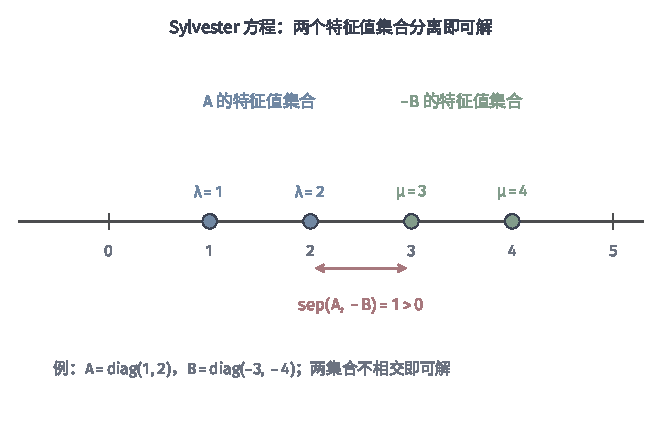
\includegraphics[width=112mm]{figures/00-shared/mathematical-preliminaries-upper/02-linear-spaces/matplotlib/ls-sylvester-separation/ls-sylvester-separation.pdf}
  \caption{Sylvester方程$\bm A\bm X+\bm X\bm B=\bm C$的特征值分离条件。
  $\bm A=\operatorname{diag}(1,2)$的特征值$\{1,2\}$与$-\bm B$（$\bm B=\operatorname{diag}(-3,-4)$）
  的特征值$\{3,4\}$在实轴上彼此分离，最近一对间距$|2-3|=1>0$，
  两集合不相交，故对任意$\bm C$有唯一解。只用实轴，不引入复数对象。}
  \label{fig:ls-sylvester-separation}
\end{figure}

\paragraph{Sylvester算子的可逆性}

一般情形的结论与对角情形相同。Sylvester算子$\mathcal L(\bm X)=\bm A\bm X+\bm X\bm B$可逆，当且仅当
\begin{equation}
\begin{gathered}
\lambda_i(\bm A)+\lambda_j(\bm B)\neq0
 \quad\text{对所有 }i,j\\
\text{即}\qquad
 \operatorname{spec}(\bm A)\cap\operatorname{spec}(-\bm B)=\varnothing,
\end{gathered}
\label{eq:ch06-sylvester-spectral-separation}
\end{equation}
其中$\operatorname{spec}$表示全体特征值，包括复特征值。实矩阵的特征值可能是复数（第~\ref{sec:ls-general-square-spectrum}节），所以条件要对全体特征值检查。

证明中会用到复特征向量。这样做是允许的：$\mathcal L$可逆等价于Kronecker矩阵~\eqref{eq:ls-sylvester-vectorized}的行列式非零，
而行列式不论在实数域还是复数域中计算都是同一个数，所以在复数域中证明齐次方程只有零解，也就证明了实算子可逆。

必要性。设条件不成立，即有$\bm A\bm u=\lambda\bm u$（$\bm u\neq\bm0$），且$-\lambda$是$\bm B$的特征值。
$\bm B^\top$与$\bm B$的特征多项式相同（$\det(\bm B^\top-\mu\bm I)=\det(\bm B-\mu\bm I)$），
所以存在$\bm w\neq\bm0$使$\bm B^\top\bm w=-\lambda\bm w$，即$\bm w^\top\bm B=-\lambda\bm w^\top$。
取$\bm X=\bm u\bm w^\top$，它不是零矩阵，而
\[
 \bm A\bm X+\bm X\bm B=(\bm A\bm u)\bm w^\top+\bm u(\bm w^\top\bm B)
 =\lambda\bm u\bm w^\top-\lambda\bm u\bm w^\top=\bm0 .
\]
齐次方程有非零解，算子不可逆。

充分性。设条件成立，且$\mathcal L(\bm X)=\bm0$，要证$\bm X=\bm0$。思路是找一个多项式$q$，
使$q(\bm A)=\bm0$而$q(-\bm B)$可逆，再利用二者与$\bm X$的关系。

第一步，把$\bm X$在两侧之间“搬运”。由$\bm A\bm X=\bm X(-\bm B)$，
得$\bm A^2\bm X=\bm A\bm X(-\bm B)=\bm X(-\bm B)^2$，归纳得$\bm A^k\bm X=\bm X(-\bm B)^k$；
对各次幂作线性组合，对任意多项式$q$有$q(\bm A)\bm X=\bm X\,q(-\bm B)$。

第二步，取$q$为$\bm A$的特征多项式$p_{\bm A}(z)=\det(z\bm I-\bm A)$。由Cayley--Hamilton定理~\ref{thm:ls-cayley-hamilton}，
$p_{\bm A}(\bm A)=\bm0$。在复数域中分解$p_{\bm A}(z)=\prod_k(z-\lambda_k)$，其中$\lambda_k$取遍$\bm A$的全部特征值，则
$p_{\bm A}(-\bm B)=\prod_k(-\bm B-\lambda_k\bm I)$。由条件~\eqref{eq:ch06-sylvester-spectral-separation}，
每个$\lambda_k$都不是$-\bm B$的特征值，所以每个因子$-\bm B-\lambda_k\bm I$都可逆，$p_{\bm A}(-\bm B)$作为可逆矩阵的乘积也可逆。

合起来，$\bm X\,p_{\bm A}(-\bm B)=p_{\bm A}(\bm A)\bm X=\bm0$，右乘$p_{\bm A}(-\bm B)^{-1}$得$\bm X=\bm0$。齐次方程只有零解，算子可逆。

至此，Sylvester方程是否对每个右端都有唯一解，完全由$\bm A$与$-\bm B$的特征值是否分离决定。
条件不成立时，方程对有些右端无解、对另一些右端有无穷多解，齐次解$\bm u\bm w^\top$给出了解不唯一的方向。

\subsection{基于Schur分解的求解}
\label{sec:ls-matrix-equation-solve}

本节统一输入$\bm A\in\mathbb R^{m\times m}$、$\bm B\in\mathbb R^{n\times n}$和$\bm C\in\mathbb R^{m\times n}$，输出满足$\bm A\bm X+\bm X\bm B=\bm C$的$\bm X$，并假定前面的谱分离条件成立。这里未知量有$mn$个元素，各方法只改变它们的组织方式；比较时应使用同一个原方程的Frobenius残差。

求解方法按$\bm A$、$\bm B$的结构分两种情况。一般情况下，方程可以化为普通线性方程直接求解，
但规模大时要用实Schur形把它约化成准三角形再逐块回代；$\bm A$、$\bm B$可对角化时，换到特征向量坐标后方程按元素分开，直接写出解。

\label{sec:ls-one-sided-two-sided}

\paragraph{向量化直接求解}

最直接的做法是形成系数矩阵~\eqref{eq:ls-sylvester-vectorized}，用第~\ref{sec:ls-direct-methods}节的LU分解求解。

具体说，按列堆叠$\bm C$得到$\bm c=\operatorname{vec}(\bm C)$，形成$\bm K=\bm I_n\otimes\bm A+\bm B^\top\otimes\bm I_m$，用带主元LU解$\bm K\bm z=\bm c$，再把$\bm z$按每$m$个元素一列还原成$\bm X$。这一步还原必须与向量化的顺序一致。
小规模问题这样做是可靠的，但系数矩阵有$(mn)^2$个元素，稠密LU约需$2(mn)^3/3$次运算；
$m=n=100$时系数矩阵已有$10^8$个元素。所以要尽量利用方程的结构，避免形成这个大矩阵。

单侧和双侧方程很容易做到。$\bm A\bm X=\bm C$是同一系数矩阵的多右端问题，对$\bm A$分解一次即可逐列复用。
双侧方程在$\bm A,\bm B$可逆时，先解$\bm A\bm Y=\bm C$，再解$\bm X\bm B=\bm Y$（即$\bm B^\top\bm X^\top=\bm Y^\top$），
也不形成Kronecker矩阵。双侧方程不相容时，可以改求$\min_{\bm X}\lVert\bm A\bm X\bm B-\bm C\rVert_{\mathrm F}^2$，
它是系数矩阵为$\bm B^\top\otimes\bm A$的最小二乘问题，由第~\ref{sec:ls-least-squares}节的方法求解。
Sylvester方程的两项相加，不能这样逐侧处理，下面借助$\bm A$、$\bm B$的正交相似变换。

\paragraph{实Schur约化}
\label{sec:ls-sylvester-schur}

正交变换不放大误差，而且由第~\ref{sec:ls-general-square-spectrum}节的实Schur形（定理~\ref{thm:ls-real-schur}），
任何实方阵都可以用正交相似化为接近三角的形状：$\bm A=\bm Q\bm T\bm Q^\top$，
$\bm Q$正交，$\bm T$是实准上三角矩阵，即对角线上是$1\times1$块（实特征值）或$2\times2$块（一对共轭复特征值），
对角块以下全为零。

分别取$\bm A=\bm Q\bm T\bm Q^\top$、$\bm B=\bm U\bm S\bm U^\top$，方程两边左乘$\bm Q^\top$、右乘$\bm U$，
利用$\bm Q^\top\bm A=\bm T\bm Q^\top$与$\bm B\bm U=\bm U\bm S$，并记$\bm Y=\bm Q^\top\bm X\bm U$、$\bm D=\bm Q^\top\bm C\bm U$，方程化为
\begin{equation}
 \bm T\bm Y+\bm Y\bm S=\bm D.
 \label{eq:ls-sylvester-transformed}
\end{equation}
正交相似不改变特征值，所以可逆条件不变；正交变换也不改变Frobenius范数，所以新坐标下的残差大小与原坐标相同。

\paragraph{准三角块上的逐块回代}

$\bm T$、$\bm S$不是对角的，方程不能按元素完全分开，但三角结构允许逐块依次求解，正如上三角方程可以回代。
按$\bm T$、$\bm S$的对角块把$\bm Y$、$\bm D$分块，比较第$(i,j)$块：
$(\bm T\bm Y)_{i,j}=\sum_k\bm T_{i,k}\bm Y_{k,j}$中只有$k\geq i$的项非零，
$(\bm Y\bm S)_{i,j}=\sum_\ell\bm Y_{i,\ell}\bm S_{\ell,j}$中只有$\ell\leq j$的项非零。
把含$\bm Y_{i,j}$的两项留在左边，其余移到右边：
\begin{equation}
 \bm T_{i,i}\bm Y_{i,j}+\bm Y_{i,j}\bm S_{j,j}
 =\bm D_{i,j}-\sum_{k>i}\bm T_{i,k}\bm Y_{k,j}
          -\sum_{\ell<j}\bm Y_{i,\ell}\bm S_{\ell,j}.
 \label{eq:ls-sylvester-block-recurrence}
\end{equation}
右边只用到同一列中更靠下的块$\bm Y_{k,j}$（$k>i$）和同一行中更靠左的块$\bm Y_{i,\ell}$（$\ell<j$）。
因此按列从左到右、每列从下到上的次序计算，每次右边需要的块都已求出。左边是一个小的Sylvester方程：
两个对角块都是$1\times1$时，它就是标量方程，直接除以$t_{i,i}+s_{j,j}$；含$2\times2$块时，它至多含$4$个未知量，
向量化后系数矩阵为$\bm I\otimes\bm T_{i,i}+\bm S_{j,j}^\top\otimes\bm I$。小块的特征值是$\bm A$、$\bm B$特征值的一部分，
由谱分离条件，每个小方程都唯一可解。

全部块求出后，由$\bm X=\bm Q\bm Y\bm U^\top$恢复原坐标，并在原坐标中计算残差$\bm A\bm X+\bm X\bm B-\bm C$。这一方法称为Bartels--Stewart算法。

两次实Schur约化的代价为$O(m^3+n^3)$，逐块回代的代价为$O(mn(m+n))$，远小于向量化直接求解的$O(m^3n^3)$；
约化只做一次，多个右端$\bm C$可以复用。

用一个已经为上三角形的例子观察回代次序。取
\[
 \bm A=\begin{bmatrix}1&1\\0&2\end{bmatrix},\qquad
 \bm B=\begin{bmatrix}3&1\\0&4\end{bmatrix},\qquad
 \bm C=\begin{bmatrix}7&12\\15&21\end{bmatrix}.
\]
此时正交因子都是单位矩阵，$\bm Y=\bm X$、$\bm D=\bm C$。按第一列从下到上计算，得到
\begin{align*}
 y_{2,1}&=15/(2+3)=3,\\
 y_{1,1}&=(7-y_{2,1})/(1+3)=1.
\end{align*}
再处理第二列：
\begin{align*}
 y_{2,2}&=(21-y_{2,1})/(2+4)=3,\\
 y_{1,2}&=(12-y_{2,2}-y_{1,1})/(1+4)=8/5.
\end{align*}
因此输出$\bm X=\left[\begin{smallmatrix}1&8/5\\3&3\end{smallmatrix}\right]$。例如原方程第$(1,2)$项为$(8/5+3)+(1+32/5)=12$，核验成立。每个右端中扣掉的量都来自已经算出的左侧或下方元素，不能同时对全部元素各除以特征值之和。

\subsection{可对角化系数的特殊情形}
\label{sec:ls-sylvester-diagonalizable}

若$\bm A$、$\bm B$可以对角化，逐块回代可以省去：换到特征向量坐标后，问题就是对角情形，有闭式解~\eqref{eq:ls-sylvester-diagonal-closed-form}。
设$\bm A=\bm V\bm\Lambda\bm V^{-1}$、$\bm B=\bm R\bm M\bm R^{-1}$，
其中$\bm\Lambda=\operatorname{diag}(\lambda_i)$、$\bm M=\operatorname{diag}(\mu_j)$。方程两边左乘$\bm V^{-1}$、右乘$\bm R$，
\[
 \bm V^{-1}\bm A\bm X\bm R+\bm V^{-1}\bm X\bm B\bm R=\bm V^{-1}\bm C\bm R .
\]
利用$\bm V^{-1}\bm A=\bm\Lambda\bm V^{-1}$与$\bm B\bm R=\bm R\bm M$，并记$\bm Y=\bm V^{-1}\bm X\bm R$、$\bm D=\bm V^{-1}\bm C\bm R$，得
\begin{equation}
\begin{gathered}
\bm\Lambda\bm Y+\bm Y\bm M=\bm D\\
y_{i,j}=\frac{d_{i,j}}{\lambda_i+\mu_j}.
\end{gathered}
\label{eq:ls-sylvester-diagonalized}
\end{equation}
最后由$\bm X=\bm V\bm Y\bm R^{-1}$变回原坐标。分母非零恰是谱分离条件~\eqref{eq:ch06-sylvester-spectral-separation}。
下面用图~\ref{fig:ls-sylvester-separation}中的两个对角矩阵算一个具体的解。

\begin{example}[对角Sylvester方程的闭式解]
\label{ex:ls-sylvester-diagonal}
取$\bm A=\operatorname{diag}(1,2)$、$\bm B=\operatorname{diag}(-3,-4)$，$\bm C$为$2\times2$的全$1$矩阵。
两个矩阵已经是对角的，可取$\bm V=\bm R=\bm I$，于是$\bm D=\bm C$。四个分母为
\[
 \begin{gathered}
1-3=-2\\
1-4=-3\\
2-3=-1\\
2-4=-2,
 \end{gathered}
\]
都不为零，由式~\eqref{eq:ls-sylvester-diagonalized}得
\[
 \bm X=\begin{bmatrix}-1/2&-1/3\\-1&-1/2\end{bmatrix}.
\]
代回可验，例如第$(1,1)$元$1\cdot(-\tfrac12)+(-\tfrac12)(-3)=1$。
\end{example}

$\bm A,\bm B$都是实对称矩阵时，特征向量可以取为标准正交的（定理~\ref{thm:ls-real-symmetric-spectral}），
此时$\bm V^{-1}=\bm V^\top$，全部计算都是实的，坐标变换也不放大误差。一般的可对角化矩阵则未必如此：
特征值可能是复数，特征向量矩阵也可能接近奇异，求逆和换坐标本身就会放大误差。
这时即使矩阵可以对角化，也宜改用一般情况的实Schur约化。

\section{李雅普诺夫方程}
\label{sec:ls-lyapunov}

李雅普诺夫方程把未知矩阵与同一线性作用的转置联系起来。下面先区分连续型与离散型，再讨论它们的求解和正定性。

\subsection{连续型与离散型方程}
\label{sec:ls-lyapunov-solvability}

Sylvester方程有一个常见的对称特例：取$\bm B=\bm A^\top$，右端记为对称矩阵$\bm Q$，得到连续型李雅普诺夫方程，即\term{Lyapunov方程}（Lyapunov equation）
\[
 \begin{gathered}
\bm A\bm X+\bm X\bm A^\top=\bm Q\\
\bm A,\bm Q\in\mathbb R^{n\times n},\ \bm Q=\bm Q^\top .
 \end{gathered}
\]
它在线性动态系统的稳定性分析与协方差计算中经常出现，所求的$\bm X$通常应当对称，有时还要求正定。
与它对应的离散型Lyapunov方程是
\[
 \bm X-\bm A^\top\bm X\bm A=\bm Q ,
\]
它不是Sylvester方程，而是双侧作用减去恒等作用；按向量化恒等式，系数矩阵为$\bm I-\bm A^\top\otimes\bm A^\top$。
本节依次回答：方程何时唯一可解，解是否对称，怎样利用对称性求解，以及解何时正定。


连续型方程是Sylvester方程的特例，可解条件可以直接读出。$\bm A^\top$与$\bm A$的特征值相同，
由谱分离条件~\eqref{eq:ch06-sylvester-spectral-separation}，算子$\bm X\mapsto\bm A\bm X+\bm X\bm A^\top$可逆，
当且仅当对$\bm A$的任意两个（可以相同的）特征值都有$\lambda_i+\lambda_j\neq0$。
取$i=j$可见，$\bm A$有零特征值时条件不成立；有一对纯虚特征值$\pm\mathrm i\omega$时也不成立。
例如$\bm A$的全部特征值实部为负时，任意两个之和的实部也为负，条件成立。

右端$\bm Q$对称且算子可逆时，解$\bm X$自动对称。对方程两边转置，得
$\bm A\bm X^\top+\bm X^\top\bm A^\top=\bm Q^\top=\bm Q$，说明$\bm X^\top$也是解；由唯一性，$\bm X=\bm X^\top$。
这只用到唯一性，不依赖任何稳定性假设。

离散型方程的齐次形式是$\bm X=\bm A^\top\bm X\bm A$。

设谱半径$\rho(\bm A)<1$，反复代入得$\bm X=(\bm A^\top)^k\bm X\bm A^k$，
而由定理~\ref{thm:ls-power-decay}，$\bm A^k\to\bm0$，所以$\bm X=\bm0$：齐次方程只有零解，方程对每个$\bm Q$唯一可解。
一般的判据是对$\bm A$的任意两个特征值都有$\lambda_i\lambda_j\neq1$，可以仿照Sylvester算子可逆性的论证证明，这里不展开。
对称性的论证与连续型相同：$\bm Q$对称时，$\bm X^\top$也是解，唯一性迫使$\bm X=\bm X^\top$。

\subsection{保持结构的求解与检验}
\label{sec:ls-lyapunov-solve}

连续型方程可以直接用Bartels--Stewart算法，而且因为$\bm B=\bm A^\top$，只需对$\bm A$作一次实Schur约化
$\bm A=\bm U\bm T\bm U^\top$，此时$\bm A^\top=\bm U\bm T^\top\bm U^\top$。

令$\bm Y=\bm U^\top\bm X\bm U$、$\bm D=\bm U^\top\bm Q\bm U$，方程化为
\[
 \bm T\bm Y+\bm Y\bm T^\top=\bm D .
\]
与递推~\eqref{eq:ls-sylvester-block-recurrence}不同，这里右侧乘的是下三角的$\bm T^\top$：
$(\bm Y\bm T^\top)_{i,j}=\sum_\ell\bm Y_{i,\ell}\bm T_{j,\ell}^\top$中只有$\ell\geq j$的项非零。于是第$(i,j)$块满足
\[
 \bm T_{i,i}\bm Y_{i,j}+\bm Y_{i,j}\bm T_{j,j}^\top
 =\bm D_{i,j}-\sum_{k>i}\bm T_{i,k}\bm Y_{k,j}-\sum_{\ell>j}\bm Y_{i,\ell}\bm T_{j,\ell}^\top ,
\]
右边用到的是同一列中更靠下的块和同一行中更靠右的块，所以要从右下角开始，按列从右到左、每列从下到上计算。

对称性还能省去一半计算。$\bm D$对称，解$\bm Y$也对称，$\bm Y_{i,\ell}=\bm Y_{\ell,i}^\top$；按这个次序只算对角线及其下方的块，
右边需要的上方块都可以由已经算出的下方块转置得到。$n\times n$的未知量因此从$n^2$个减为$n(n+1)/2$个。
最后由$\bm X=\bm U\bm Y\bm U^\top$变回原坐标。

离散型方程同样先作约化，得$\bm Y-\bm T^\top\bm Y\bm T=\bm D$。比较第$(i,j)$块，
$(\bm T^\top\bm Y\bm T)_{i,j}=\sum_{k\leq i,\ \ell\leq j}\bm T_{k,i}^\top\bm Y_{k,\ell}\bm T_{\ell,j}$，
依赖的是行、列下标都不超过$(i,j)$的块。因此递推要从左上角开始，按列从左到右、每列从上到下计算。把当前块留在左边，得到
\[
 \bm Y_{i,j}-\bm T_{i,i}^\top\bm Y_{i,j}\bm T_{j,j}
 =\bm D_{i,j}+\sum_{\substack{k\leq i,\ \ell\leq j\\(k,\ell)\ne(i,j)}}
 \bm T_{k,i}^\top\bm Y_{k,\ell}\bm T_{\ell,j}.
\]
右边的块已经计算完毕。记其和为$\bm F_{i,j}$，对当前小块按列向量化，解
\[
 (\bm I-\bm T_{j,j}^\top\otimes\bm T_{i,i}^\top)
 \operatorname{vec}(\bm Y_{i,j})=\operatorname{vec}(\bm F_{i,j}).
\]
每个对角块至多为二阶，故一次至多解四个未知量。全部块求出后，仍由$\bm X=\bm U\bm Y\bm U^\top$恢复。块之间的依赖关系与连续型不同，不能照搬连续型的递推次序。

两种算法都输入$\bm A$和对称右端$\bm Q$，输出$\bm X$。结束时，连续型检查$\bm A\bm X+\bm X\bm A^\top-\bm Q$，离散型检查$\bm X-\bm A^\top\bm X\bm A-\bm Q$，并同时检查$\bm X-\bm X^\top$；仅看还原后的矩阵是否对称，不能判断它是否解了正确的方程。

\subsection{正定解及其条件}
\label{sec:ls-lyapunov-positivity}

对称的解是否正定，是比可解性更强的问题。下面的充分条件都要求右端定号，并要求$\bm A$满足稳定性条件。

离散型方程在$\rho(\bm A)<1$时可以把解直接写出来。方程可以改写成$\bm X=\bm Q+\bm A^\top\bm X\bm A$，
反复代入右边的$\bm X$，就是把每步的作用$\bm X\mapsto\bm A^\top\bm X\bm A$反复施加在$\bm Q$上并累加，
这与第~\ref{sec:ls-matrix-series-exponential}节的Neumann级数同出一辙。于是考虑
\begin{equation}
 \bm X=\sum_{k=0}^{\infty}(\bm A^{\top})^k\bm Q\bm A^k .
 \label{eq:ls-discrete-lyapunov-series}
\end{equation}
取$r$满足$\rho(\bm A)<r<1$，由引理~\ref{lem:ls-power-geometric-bound}，存在常数$C_r$使$\lVert\bm A^k\rVert_2\leq C_rr^k$，
所以第$k$项的范数不超过$\lVert\bm Q\rVert_2\lVert\bm A^k\rVert_2^2\leq\lVert\bm Q\rVert_2C_r^2r^{2k}$，级数按几何级数收敛。
它满足方程：逐项计算，$\bm A^\top\bm X\bm A=\sum_{k\geq1}(\bm A^\top)^k\bm Q\bm A^k$，与$\bm X$相减只剩$k=0$项$\bm Q$。
由第~\ref{sec:ls-lyapunov-solvability}节的唯一性，级数~\eqref{eq:ls-discrete-lyapunov-series}就是方程的唯一解。

标量情形最容易核对。

\begin{example}[标量离散Lyapunov方程]
\label{ex:ls-scalar-discrete-lyapunov}
取$n=1$、$\bm A=a$、$\bm Q=q$，$|a|<1$。级数~\eqref{eq:ls-discrete-lyapunov-series}是公比为$a^2$的几何级数：
\[
 x=\sum_{k=0}^{\infty}a^{2k}q=\frac{q}{1-a^2}.
\]
代入方程，$x-a^2x=(1-a^2)\dfrac{q}{1-a^2}=q$，恰好成立。$q>0$时$x>0$，与下面的正定性结论一致。
\end{example}

这一表示直接给出正定性。若$\bm Q\succ0$，则对$\bm x\neq\bm0$，
\[
 \bm x^\top\bm X\bm x=\sum_{k=0}^{\infty}(\bm A^k\bm x)^\top\bm Q(\bm A^k\bm x)\geq\bm x^\top\bm Q\bm x>0 ,
\]
解正定；$\bm Q\succeq0$时每一项都非负，同理得$\bm X\succeq0$。

连续型的对应结论是：$\bm A$的全部特征值实部为负、右端负定，即$\bm A\bm X+\bm X\bm A^\top=-\bm W$且$\bm W\succ0$时，解$\bm X$正定。
它的证明要把解写成积分$\int_0^\infty e^{t\bm A}\bm W e^{t\bm A^\top}\,\mathrm dt$，本卷不展开。
实际计算时不必依赖这些表示：对算出的$\bm X$作Cholesky分解，分解成功即说明$\bm X\succ0$（第~\ref{sec:ls-direct-methods}节）。

\section{本章小结}
\label{sec:ls-equations-summary}

本章讨论了三个反求输入的问题：线性方程$\bm A\bm x=\bm b$、Sylvester方程$\bm A\bm X+\bm X\bm B=\bm C$与Lyapunov方程$\bm A\bm X+\bm X\bm A^\top=\bm Q$。
三者都是有限维空间上的线性方程，都先判断解的情况，再求解。

线性方程的情况由秩判别：$\operatorname{rank}[\bm A\;\bm b]=\operatorname{rank}(\bm A)$时有解，全部解是一个特解加$\operatorname{null}(\bm A)$。
唯一解按矩阵结构用LU、Cholesky或LDL$^{\top}$等直接法算出；有无穷多解时须声明准则，欧氏范数最小的解落在$\operatorname{range}(\bm A^\top)$中。

对大型方程，定常迭代使用固定修正规则，其收敛由迭代矩阵的谱半径判定；CG、MINRES与GMRES分别适用于对称正定、对称不定和一般非对称方程，在逐步扩大的子空间内选择近似；BiCG与BiCGSTAB使用不同的短递推。

无解时改求最小二乘，残差与列空间正交给出总是相容的正规方程。LSQR与LSMR利用双对角化逐步求解，分别控制原残差与正规残差，逐行投影则适合按行访问数据，但不相容方程需要扩展。伪逆把三种答案统一为$\bm A^\dagger\bm b$。

数据有误差时，条件数刻画解的放大，根源是小奇异值，形成正规方程还会把条件数平方。
岭回归与截断SVD以增加残差为代价压低或丢弃小奇异值方向；修正Gram--Schmidt、Householder反射与Givens旋转不改变问题，只让计算更稳定。

Sylvester方程对任意右端唯一可解，当且仅当$\bm A$与$-\bm B$没有公共特征值；求解时不形成Kronecker系数矩阵，而用实Schur约化后逐块回代。
连续型Lyapunov方程是$\bm B=\bm A^\top$的特例，对称右端的解由唯一性保证对称，求解只需一次约化、只算一半的块；
离散型方程在$\rho(\bm A)<1$时有级数解，由它可读出$\bm Q\succ0$时解正定。

